\documentclass[twoside,11pt]{article}

% Any additional packages needed should be included after jmlr2e.
% Note that jmlr2e.sty includes epsfig, amssymb, natbib and graphicx,
% and defines many common macros, such as 'proof' and 'example'.
%
% It also sets the bibliographystyle to plainnat; for more information on
% natbib citation styles, see the natbib documentation, a copy of which
% is archived at http://www.jmlr.org/format/natbib.pdf

\usepackage{jmlr2e}

\usepackage{algpseudocode}
\usepackage{algorithm}
\usepackage{amsmath}
\usepackage{amssymb}
\usepackage{float}
\usepackage{graphicx}
\usepackage{multirow}
\usepackage[caption = false]{subfig}

% Definitions of handy macros can go here

\newcommand{\dataset}{{\cal D}}
\newcommand{\fracpartial}[2]{\frac{\partial #1}{\partial  #2}}

% Heading arguments are {volume}{year}{pages}{submitted}{published}{author-full-names}

\jmlrheading{1}{2016}{1-48}{4/00}{10/00}{Theodore Papamarkou and Eric Ford}

% Short headings should be running head and authors last names

\ShortHeadings{Manifold Langevin Monte Carlo with Partial Metric Updates}{Papamarkou and Ford}
\firstpageno{1}

\begin{document}

\title{Manifold Langevin Monte Carlo with Partial Metric Updates}

\author{
  \name Theodore Papamarkou
  \email theodore.papamarkou@glasgow.ac.uk\\
  \addr 
    School of Mathematics and Statistics\\
    University of Glasgow\\
    15 University Gardens\\
    Glasgow, G12 8QW, UK
\AND
  \name Eric B. Ford
  \email ebf11@psu.edu\\
  \addr
    Center for Astrostatistics\\
    Institute for CyberScience\\
    Center for Exoplanets and Habitable Worlds\\
    Department of Astronomy and Astrophysics\\
    525 Davey Lab\\
    The Pennsylvania State University\\
    University Park, PA 16802, USA
}

\editor{Leslie Pack Kaelbling}

\maketitle

\begin{abstract}%   <- trailing '%' for backward compatibility of .sty file
Manifold Markov chain Monte Carlo algorithms have been introduced to sample more effectively from challenging target 
densities exhibiting multiple modes or strong correlations. Such algorithms exploit the local geometry of the parameter 
space, thus enabling chains to achieve a faster convergence rate when measured in number of steps. However, often acquiring 
local geometric information increases computational complexity per step to the extent that sampling from high-dimensional 
targets becomes inefficient in terms of total computational time. This paper proposes a manifold Langevin Monte Carlo 
framework aimed at balancing the benefits of exploiting local geometry with computational requirements to achieve a high 
effective sample size for a given computational cost. The suggested strategy regulates the frequency of manifold-based 
updates via a schedule. An exponentially decaying schedule is put forward that enables more frequent updates of geometric 
information in early transient phases of the chain, while saving computational time in late stationary phases. 
Alternatively, a modulo schedule is introduced to allow for infrequent yet recurring geometric updates throughout the 
sampling course, acting to adaptively update proposals to learn the covariance structure of the parameter space. The average 
complexity can be manually set for either of these two schedules depending on the need for geometric exploitation posed by 
the underlying model.  
\end{abstract}

\begin{keywords}
  Bayesian inference,
  High-dimensional data analysis,
  Markov chain Monte Carlo,
  Langevin Monte Carlo	
\end{keywords}

\section{Introduction}

The birth of geometric-based Markov chain Monte Carlo (MCMC) dates back to the landmark paper of \cite{dua_ken_pen__hyb},
which introduced Hamiltonian Monte Carlo (HMC) to unite MCMC with molecular dynamics.
\cite{dua_ken_pen__hyb} applied HMC in lattice field theory simulations of quantum chromodynamics.
Statistical applications of HMC began with its use in neural network models by \cite{nea__bay}.

In the meanwhile, the Metropolis-adjusted Langevin algorithm (MALA) was proposed by \cite{rob_ros__opt} to harness Langevin 
dynamics for proposing new states in MCMC simulations. Both HMC and MALA evaluate the gradient of the target density, so 
they utilize local geometric flow.

The seminal work of \cite{gir_cal__rie} raised awareness of the differential geometric foundations of MCMC. Given a vector 
of parameters $\boldsymbol{\theta}\in\mathbb{R}^{n_\theta}$, \cite{gir_cal__rie} defines a distance between two probability 
densities $p(\boldsymbol{\theta})$ and $p(\boldsymbol{\theta}+\delta\boldsymbol{\theta})$ as the quadratic form
$\delta\boldsymbol{\theta}^T G(\boldsymbol{\theta}) \delta\boldsymbol{\theta}$ for an arbitrary metric 
$G(\boldsymbol{\theta})$. Thus, the position-specific metric $G(\boldsymbol{\theta})$ induces a Riemann manifold in the 
space of parameterized probability density functions $\left\{p(\boldsymbol{\theta}):\boldsymbol{\theta}\right\}$.
In the context of MCMC, $G(\boldsymbol{\theta})$ depends on the current state $\boldsymbol{\theta}$ of the simulated Markov 
chain. \cite{gir_cal__rie} uses $G(\boldsymbol{\theta})$ to define transition kernels that explore the parameter space
$\left\{\boldsymbol{\theta}:\boldsymbol{\theta}\in\mathbb{R}^{n_\theta}\right\}$ effectively, thereby introducing Riemann 
manifold Langevin and Hamiltonian Monte Carlo methods.

The differential geometric basis of MCMC has been further researched since the appearance of \cite{gir_cal__rie}. For 
instance, \cite{byr_gir__geo} developed proposal mechanisms by following geodesic flows over the embedded manifolds of 
support for the target distribution. \cite{lan_sta_sha__mar} replaced the auxiliary momentum variable appearing in Riemann 
manifold Hamiltonian Monte Carlo (RMHMC) by velocity to develop a Markov chain Monte Carlo algorithm using Lagrangian 
dynamics. \cite{lan_str_sha__wor} defined the so-called wormhole metric, for which distance between modes is shortened, in 
order to facilitate transitions between modes of multimodal target densities.

Computing the geometric entities of differential geometric MCMC methods creates a performance bottleneck that restricts the 
applicability of the involved methods. For example, manifold Monte Carlo methods require to calculate the metric tensor
$G(\boldsymbol{\theta})$ of choice. Typically, $G(\boldsymbol{\theta})$ is set to be the observed Fisher information matrix,
which equals the negative Hessian of the log-target density at a specific point $\boldsymbol{\theta}$. Consequently, the 
complexity of manifold MCMC algorithms is dominated by Hessian-related computations, either the computation of gradient and 
Hessian or the inversion of the Hessian.  

\cite{gir_cal__rie} introduced the simplified manifold Metropolis-adjusted Langevin algorithm (SMMALA) that is of the same 
order but often faster than MMALA and RMHMC in lower-dimensional parameter spaces. The faster speed of SMMALA over MMALA and 
RMHMC is explained by lower order terms and constant factors appearing in big-oh notation, which are ordinarily omitted but 
affect runtime in the case of smaller $n_\theta$. For this reason, SMMALA has been employed in conjunction with population 
MCMC for the Bayesian analysis of mechanistic models based on systems of non-linear differential equations, see 
\cite{cal_gir__sta} and \cite{sch_pap__ews}. Despite the capacity of SMMALA to exploit local geometric information so as to 
cope with non-linear correlations and modest increase in the dimensionality of the parameter space, in other cases its 
computational complexity can render the performance inferior to other algorithms such as the Metropolis-adjusted Langevin 
algorithm (MALA) or adaptive MCMC, see \cite{cal_eps_sil__bay}.

Various attempts have been made to ameliorate the computational implications of geometric Monte Carlo methods. Along these 
lines, \cite{lan_tha_chr__emu} used Gaussian processes to emulate the Hessian matrix and Christoffel symbols associated with 
the observed Fisher information $G(\boldsymbol{\theta})$. \cite{sim_bad_cem__sto} developed a stochastic quasi-Newton 
Langevin MCMC algorithm which takes into account the local geometry, while approximating the inverse Hessian by using a 
limited history of samples and their gradients. Alternatively, \cite{per__prox} used convex analysis and proximal techniques 
instead of differential calculus in order to construct a Langevin Monte Carlo method for high-dimensional target 
distributions that are log-concave and possibly not continuously differentiable.

This paper develops a Monte Carlo method that improves on the sampling efficacy of SMMALA, while remaining simple to 
implement. The proposed method permits adjustments to the metric updates and at the same time has smaller computational cost 
than SMMALA. Moreover, the suggested algorithm performs exact metric evaluations, avoiding emulation or other approximations 
of the Hessian of the log-target density.

\section{Background}

The role of this section is to provide a brief overview of Langevin Monte Carlo and to stage a unified notation, which will
be used for introducing the method contributed by this paper.

From a statistical perspective, Langevin Monte Carlo is a special case of Metropolis-Hastings with a normal proposal
distribution
\begin{equation}
\label{langevin_proposal}
q(\boldsymbol{\theta}^{\star}|\boldsymbol{\theta}) =
\mathcal{N}(\boldsymbol{\theta}^{\star}|\boldsymbol{\mu}(\boldsymbol{\theta}, G, \epsilon), \Sigma(G, \epsilon)),
\end{equation}
where $\boldsymbol{\theta}^{\star}$ and $\boldsymbol{\theta}$ denote the respective proposed and current state, $G$ is a
positive definite matrix of size $n_{\theta} \times n_{\theta}$ and $\epsilon$ refers to a tuning parameter known as the
integration stepsize. The location $\boldsymbol{\mu}(\boldsymbol{\theta}, G, \epsilon)$ is a function of 
$\boldsymbol{\theta}$, $G$ and $\epsilon$, whereas the covariance $\Sigma(G, \epsilon)$ of the proposal density depends on 
$G$ and $\epsilon$. Both $\boldsymbol{\mu}(\boldsymbol{\theta}, G, \epsilon)$ and $\Sigma(G, \epsilon)$ are defined so that 
the proposed states admit a Langevin diffusion approximated by a first-order Euler discretization. In other words, the 
Langevin diffusion has a stationary distribution $p(\boldsymbol{\theta})$, so a Markov chain simulated from the 
Metropolis-Hastings scheme outlined by proposal \eqref{langevin_proposal} will converge to the target 
$p(\boldsymbol{\theta})$. The Metropolis-Hastings acceptance probability is set to its standard form
\begin{equation}
\label{langevin_acceptance}
a(\boldsymbol{\theta},\boldsymbol{\theta}^{\star}) =
\min\left\{
\frac{p(\boldsymbol{\theta}^{\star})q(\boldsymbol{\theta}|\boldsymbol{\theta}^{\star})}
{p(\boldsymbol{\theta})q(\boldsymbol{\theta}^{\star}|\boldsymbol{\theta})}
, 1
\right\}.
\end{equation}

The integration stepsize $\epsilon$, also known as drift step, is associated with the first order Euler discretization and 
significantly affects the rate of state space exploration. If $\epsilon$ is selected to be relatively large, many of the 
proposed candidates will be far from the current state, and are likely to have a low probability of acceptance, so the 
generated chain will have low acceptance rate. Reducing $\epsilon$ will increase the acceptance rate, but the chain will 
take longer to traverse the state space.

In a Bayesian setting, the target is a possibly unnormalized posterior distribution $p(\boldsymbol{\theta}|\mathbf{y})$,
where $\mathbf{y}$ denotes the available data. Replacing $p(\boldsymbol{\theta})$ by $p(\boldsymbol{\theta}|\mathbf{y})$ in
\eqref{langevin_acceptance} makes Langevin Monte Carlo applicable in Bayesian problems.

To fully specify a Langevin Monte Carlo algorithm, the location $\boldsymbol{\mu}(\boldsymbol{\theta}, G, \epsilon)$ and 
covariance $\Sigma(G, \epsilon)$ of normal proposal \eqref{langevin_proposal} need to be defined. In what follows, 
variations of geometric Langevin Monte Carlo methods are distinguished by their respective proposal location and covariance.

\subsection{Metropolis-Adjusted Langevin Algorithm}
\label{mala_section}

If $G$ is kept constant, that is if $G$ is a not a function of the current state $\boldsymbol{\theta}$, then the
Metropolis-adjusted Langevin algorithm (MALA) arises as
\begin{eqnarray}
\label{mala_location}
\boldsymbol{\mu}(\boldsymbol{\theta}, G, \epsilon) = 
\boldsymbol{\theta}+\frac{\epsilon^2}{2}G^{-1}\nabla_{\theta}\log{p(\boldsymbol{\theta})},\\
\label{mala_covariance}
\Sigma(G, \epsilon) = \epsilon^2 G^{-1}.
\end{eqnarray}
$G$ is known as the precondition matrix, see \cite{rob_stra__lan}. It is typically set to be the identity matrix $G=I$, in
which case MALA is defined in its conventional form
\begin{equation}
\label{mala_location_covariance_identity}
\boldsymbol{\mu}(\boldsymbol{\theta}, \epsilon) = 
\boldsymbol{\theta}+\frac{\epsilon^2}{2}\nabla_{\theta}\log{p(\boldsymbol{\theta})},~
\Sigma(\epsilon) = \epsilon^2 I.
\end{equation}

MALA uses the gradient flow $\nabla_{\theta}\log{p(\boldsymbol{\theta})}$ to make proposals effectively. According to the 
theoretical analysis of \cite{rob_ros__opt}, the optimal scaling $\epsilon$ has been found to be the value of $\epsilon$ 
which yields a limiting acceptance rate of $57.4\%$ in high-dimensional parametric spaces (as $n_{\theta}\rightarrow\infty$).

\subsection{Manifold Langevin Monte Carlo Algorithms}
\label{smmala_section}

It is possible to incorporate further geometric structure in the form of a position-dependent metric 
$G(\boldsymbol{\theta})$, as explained by \cite{gir_cal__rie}. The Langevin diffusion is defined on a Riemann manifold 
endowed by the metric $G(\boldsymbol{\theta})$, and the corresponding Levi-Civita connection specified by the Christoffel 
symbols of second-kind $\Gamma^{k}_{ij}(\boldsymbol{\theta})$. The resulting manifold Metropolis-adjusted Langevin algorithm 
(MMALA) draws candidate states from a normal proposal with location and covariance given by
\begin{eqnarray}
\label{mmala_location}
\boldsymbol{\mu}_{(k)}(\boldsymbol{\theta}, G(\boldsymbol{\theta}), \epsilon) =
\boldsymbol{\theta}+
\frac{\epsilon^2}{2}(G^{-1}(\boldsymbol{\theta})\nabla_{\theta}\log{p(\boldsymbol{\theta})})_{(k)}-
\epsilon^2\sum_{i,j=1}^{n_\theta}G^{-1}_{ij}(\boldsymbol{\theta})\Gamma^{k}_{ij}(\boldsymbol{\theta}),\\
\label{mmala_covariance}
\Sigma(G(\boldsymbol{\theta}), \epsilon) = \epsilon^2 G^{-1}(\boldsymbol{\theta}),
\end{eqnarray}
where $\boldsymbol{\mu}_{(k)}$ refers to the $k$-th coordinate of proposal location
$\boldsymbol{\mu}(\boldsymbol{\theta}, G(\boldsymbol{\theta}), \epsilon)$.

If a manifold of constant curvature is assumed, then the Christoffel symbols vanish, significantly reducing the complexity 
of calculations needed for complex models. In this case, the proposal location of MMALA simplifies to
\begin{equation}
\label{smmala_location}
\boldsymbol{\mu}(\boldsymbol{\theta}, G(\boldsymbol{\theta}), \epsilon) =
\boldsymbol{\theta}+
\frac{\epsilon^2}{2}G^{-1}(\boldsymbol{\theta})\nabla_{\theta}\log{p(\boldsymbol{\theta})}.
\end{equation}
The method with location and covariance specified by \eqref{smmala_location} and \eqref{mmala_covariance} is known as 
simplified Metropolis-adjusted Langeving algorithm (SMMALA). As seen from the location and covariance of their proposal 
mechanisms, MALA is a special case of SMMALA, which is in turn a special case of MMALA.

The optimal stepsize $\epsilon$ for MMALA and SMMALA is empirically suggested by \cite{gir_cal__rie} to be set so as to 
obtain an acceptance rate of around $70\%$; this choice has not been analyzed yet from a theoretical standpoint analogously 
to the choice of scaling for MALA by \cite{rob_ros__opt}. Even if the curvature of the target density is not strictly 
constant, SMMALA can be applied and may be more efficient than MMALA.

\subsection{Computational Complexity}
\label{Motivation}

Calculations associated with the proposal and target densities determine the incurring computational cost of Langevin 
Monte Carlo methods. In brief, the main computational requirements include sampling from and evaluating the proposal, as well
as evaluating the target and its derivatives.

Ordinarily, the proposal used in Langevin Monte Carlo is set to be a multivariate normal distribution
$
q(\boldsymbol{\theta}^{\star}|\boldsymbol{\theta}) =
\mathcal{N}(\boldsymbol{\theta}^{\star}|
\boldsymbol{\mu}(\boldsymbol{\theta}, G, \epsilon), \epsilon^2 G^{-1}(\boldsymbol{\theta}))
$,
as seen in \eqref{langevin_proposal}, \eqref{mala_covariance} and \eqref{mmala_covariance}. To propose a state 
$\boldsymbol{\theta}^{\star}$, the proposal is typically simulated in the Cholesky approach by letting
\begin{equation}
\boldsymbol{\theta}^{\star} =
\boldsymbol{\mu}(\boldsymbol{\theta}, G, \epsilon)+
\epsilon \left(\sqrt{G^{-1}(\boldsymbol{\theta})}\right)^{'}\tau
\end{equation}
where $\sqrt{G^{-1}(\boldsymbol{\theta})}$ satisfies the Cholesky decomposition
$
\left(\sqrt{G^{-1}(\boldsymbol{\theta})}\right)^{'}\sqrt{G^{-1}(\boldsymbol{\theta})}=
G^{-1}(\boldsymbol{\theta})
$
and $\tau\sim\mathcal{N}(\mathbf{0}, I)$, \cite{chi_gre__und}.
So, sampling from the proposal has a complexity of $\mathcal{O}(2n_\theta^3)$, since it requires the inversion of metric 
$G(\boldsymbol{\theta})$ and the Cholesky decomposition of $G^{-1}(\boldsymbol{\theta})$, each of which are
$\mathcal{O}(n_\theta^3)$ operations.

To calculate the Metropolis-Hastings acceptance ratio \eqref{langevin_acceptance} appearing in SMMALA and MMALA,
it is required to evaluate the normal proposal twice. As it has become apparent, a proposal evaluation has a complexity of
$\mathcal{O}(n_\theta^3)$ due to the proposal covariance $\epsilon^2 G^{-1}(\boldsymbol{\theta})$ entailing the inversion of 
$G(\boldsymbol{\theta})$.

So, SMMALA and MMALA necessitate computing the two matrix inverses $G^{-1}(\boldsymbol{\theta})$ and 
$G^{-1}(\boldsymbol{\theta}^{\star})$ in order to evaluate the proposals involved in the acceptance probability 
\eqref{langevin_acceptance}, and one Cholesky decomposition $\sqrt{G^{-1}(\boldsymbol{\theta})}$ to sample from the 
proposal. Consequently, the cost of computations associated with the normal proposal is of order $\mathcal{O}(3n_\theta^3)$ 
for each of these two samplers.

Owing to the works of \cite{dav_sto__imp}, \cite{wil__brea} and \cite{leg__pow},
optimized versions of the Coppersmith-Winograd algorithm allow to perform matrix multiplication and therefore matrix 
inversion in $\mathcal{O}(n_\theta^{2.373})$ time. Hence, optimized implementations of SMMALA and MMALA can each run their
proposal-related computations in $\mathcal{O}(n_\theta^3+2n_\theta^{2.373})$ and time.

MALA, as opposed to SMMALA and MMALA, relies on a constant preconditioning matrix $G$, therefore $G^{-1}$ and 
$\sqrt{G^{-1}}$ are evaluated once and cached at the beginning of the simulation avoiding the $\mathcal{O}(2n_\theta^3)$ 
penalty. Since the preconditioning matrix $G$, its inverse $G^{-1}$ and the Cholesky decomposition $\sqrt{G^{-1}}$ are 
cached upon initialization for MALA, the quadratic form
$
(\boldsymbol{\theta}^{\star}-\boldsymbol{\theta}^{\star})'
G^{-1}
(\boldsymbol{\theta}^{\star}-\boldsymbol{\theta}^{\star})
$
in the normal proposal density dictates a time complexity of $\mathcal{O}(n_{\theta}^2)$ for proposal-related computations
in MALA. If $G$ is set to be the identity matrix, then
$
(\boldsymbol{\theta}^{\star}-\boldsymbol{\theta}^{\star})'
G^{-1}
(\boldsymbol{\theta}^{\star}-\boldsymbol{\theta}^{\star})
$
reduces to the inner product
$
\langle\boldsymbol{\theta}^{\star}-\boldsymbol{\theta}^{\star},
\boldsymbol{\theta}^{\star}-\boldsymbol{\theta}^{\star}\rangle
$ and the complexity of calculations associate wit the proposal in MALA is of order $\mathcal{O}(n_{\theta})$.

If a log-target has a complexity of order $\mathcal{O}(f(n_{\theta}))$, where $f$ is a function of $n_{\theta}$, then the 
complexity orders for computations associated with the log-target in MALA, SMMALA and MMALA grow as 
$\mathcal{O}(f(n_{\theta})n_{\theta})$, $\mathcal{O}(f(n_{\theta})n_\theta^2)$ and $\mathcal{O}(f(n_{\theta})n_{\theta}^3)$, 
respectively. These incurring costs for MALA, SMMALA and MMALA arise from the respective evaluations of log-target gradient, 
Hessian and Hessian derivatives.

Adding up the cost of computations associated with the proposal and the target yields the order of complexity for Langevin
Monte Carlo. So, it follows that MALA, SMMALA and MMALA run in $\mathcal{O}(f(n_{\theta})n_{\theta}+n_\theta^2)$, 
$\mathcal{O}(f(n_{\theta})n_\theta^2+n_\theta^3+2n_\theta^{2.373})$ and 
$\mathcal{O}(f(n_{\theta})n_{\theta}^3+n_\theta^3+2n_\theta^{2.373})$ time, respectively.

For simple models, the order of complexity of the log-target is not greater than that of the proposal, so it is assumed that
the log-target scales as $\mathcal{O}(1)$. Thus, for simple models, the respective complexity bounds for MALA, SMMALA and
MMALA reduce to $\mathcal{O}(n_{\theta}^2)$, $\mathcal{O}(n_{\theta}^2)$ and $\mathcal{O}(n_{\theta}^3)$ after dropping
scaling factors and lower-order terms. The complexity order of the typical MALA with identity preconditioning matrix further
reduces to $\mathcal{O}(n_{\theta})$ for a simple model.

On the other hand, computationally expensive models imply $\mathcal{O}(f(n_{\theta}))>>\mathcal{O}(n_{\theta})$. For such
models, the cost of computations implicating the log-target is much higher than the cost of proposal-related calculation. In 
other words, if the log-target is of high complexity, then derivative computations supersede linear algebra calculations, 
and this is why the computational cost of a manifold MCMC algorithm tends to be reported as a function of the order of 
derivatives appearing in the algorithm. For instance, the complexity of SMMALA, which scales as 
$\mathcal{O}(f(n_{\theta})n_\theta^2+n_\theta^3+2n_\theta^{2.373})$, can be simply written as $\mathcal{O}(f^2(n_{\theta}))$ 
for a computationally intensive model.

A typical example of a computationally expensive model is a system of non-linear ordinary differential equations (ODEs), 
where each log-target calculation requires solving the ODE system numerically. It is then expected that the log-target and 
its derivative evaluations will dominate the cost of Langevin Monte Carlo simulations according to the discussed complexity
bounds.

A detailed account of the time complexity of SMMALA has been given to highlight the main sources of computational load
involved in geometric updates. In what follows, scaling factors and constants will be suppressed in big-$\mathcal{O}$ 
notation following common practice.

Combining the best of two worlds, an effective and efficient MCMC algorithm would exploit geometric information in time as 
close as possible to the linear time of MALA. One potential approach towards this end would be to approximate the expensive 
components of geometric computation, such as $G^{-1}(\boldsymbol{\theta})$ and $\sqrt{G^{-1}(\boldsymbol{\theta})}$, in the 
spirit of \cite{sim_bad_cem__sto}. An alternative route, taken by the present paper, is to design a hybrid sampling method 
that switches between expensive geometrically-informed and cheaper non-geometric proposal mechanisms. The latter idea is
motivated by the objective to exploit exact geometric updates whenever these occur, therefore not rendering each Monte Carlo 
iteration approximate.

\section{Partial Manifold Langevin Metric Updates}

\subsection{Partial Manifold Langevin Metric Updates in MALA}

Sections \ref{mala_section} and \ref{smmala_section} provide a unified formulation of MALA and SMMALA. More specifically, 
both samplers constitute variations of a Metropolis-Hastings algorithm with a normal proposal given by 
\eqref{langevin_proposal} and acceptance probability defined by \eqref{langevin_acceptance}. The MALA and SMMALA normal 
proposals differ in their locations and covariances, which are specified by \eqref{mala_location}-\eqref{mala_covariance} 
and \eqref{smmala_location}-\eqref{mmala_covariance} respectively. From an algorithmic perspective, the natural way to 
switch between MALA and SMMALA updates is to variably rely on the locations and covariances of their associated 
candidate-generating kernels.

Both MALA and SMMALA learn from the local geometry of the underlying manifold. MALA resorts to gradient flow computations, 
while SMMALA further enriches its geometric information by incorporating the position-specific metric 
$G(\boldsymbol{\theta})$ to the updating mechanism. So, strictly speaking, a hybrid algorithm that switches between MALA and 
SMMALA proposals combines two geometric MCMC methods with varying levels of geometric information and of computational cost. 
To keep the resulting complexity as low as possible, the bulk of transitions should be driven by MALA, allowing intervening 
SMMALA updates to occur just frequently enough to boost sampling effectiveness.

A first question is how to pick from the MALA and SMMALA proposals at each MCMC iteration. One possibility is to make a
random choice via a Bernoulli trial. At the $i$-th iteration, draw a sample $b(i)\sim \mbox{Bernoulli}(p(i))$ with
probability $p(i)$ of taking a SMMALA step. If $b(i)=0$ then propose a new state $\boldsymbol{\theta}^{\star}$ sampled from
the MALA proposal, whereas if $b(i)=1$ then propose $\boldsymbol{\theta}^{\star}$ drawn from the SMMALA proposal.

Secondly, there needs to be a way of selecting the probabilities $p(i)$ as a function of the current iteration
$i\in\left\{1,2,\cdots,n_m\right\}$, where $n_m$ is the total number of MCMC steps. In other words, a schedule is needed for
the probabilities $p(i)$ of choosing between MALA and SMMALA updates. One possible choice of $p(i)$ is an exponentially 
decaying schedule
\begin{equation}
\label{exp_schedule_a}
p(i)=\exp{(-a(i-1)/n_m)},
\end{equation}
where $a$ denotes a constant tuning factor that determines the decay rate of $p(i)$.
Schedule \eqref{exp_schedule_a} makes SMMALA updates more probable in early transient iterations of the chain, while it 
makes MALA updates increasingly more likely in late stationary iterations. Hence, as the chain converges, less geometric 
information is acquired to reduce the computational load. Figure \ref{fig:exp_schedule_a} displays the schedule of Bernoulli 
probabilities for varying decaying rates.  This schedule is likely to be efficient for problems well approximated by a 
single metric, even if an appropriate metric is not known a priori.

\begin{figure}[t]
	\centering
	\subfloat[$b=0$]{
		\label{fig:exp_schedule_a}
		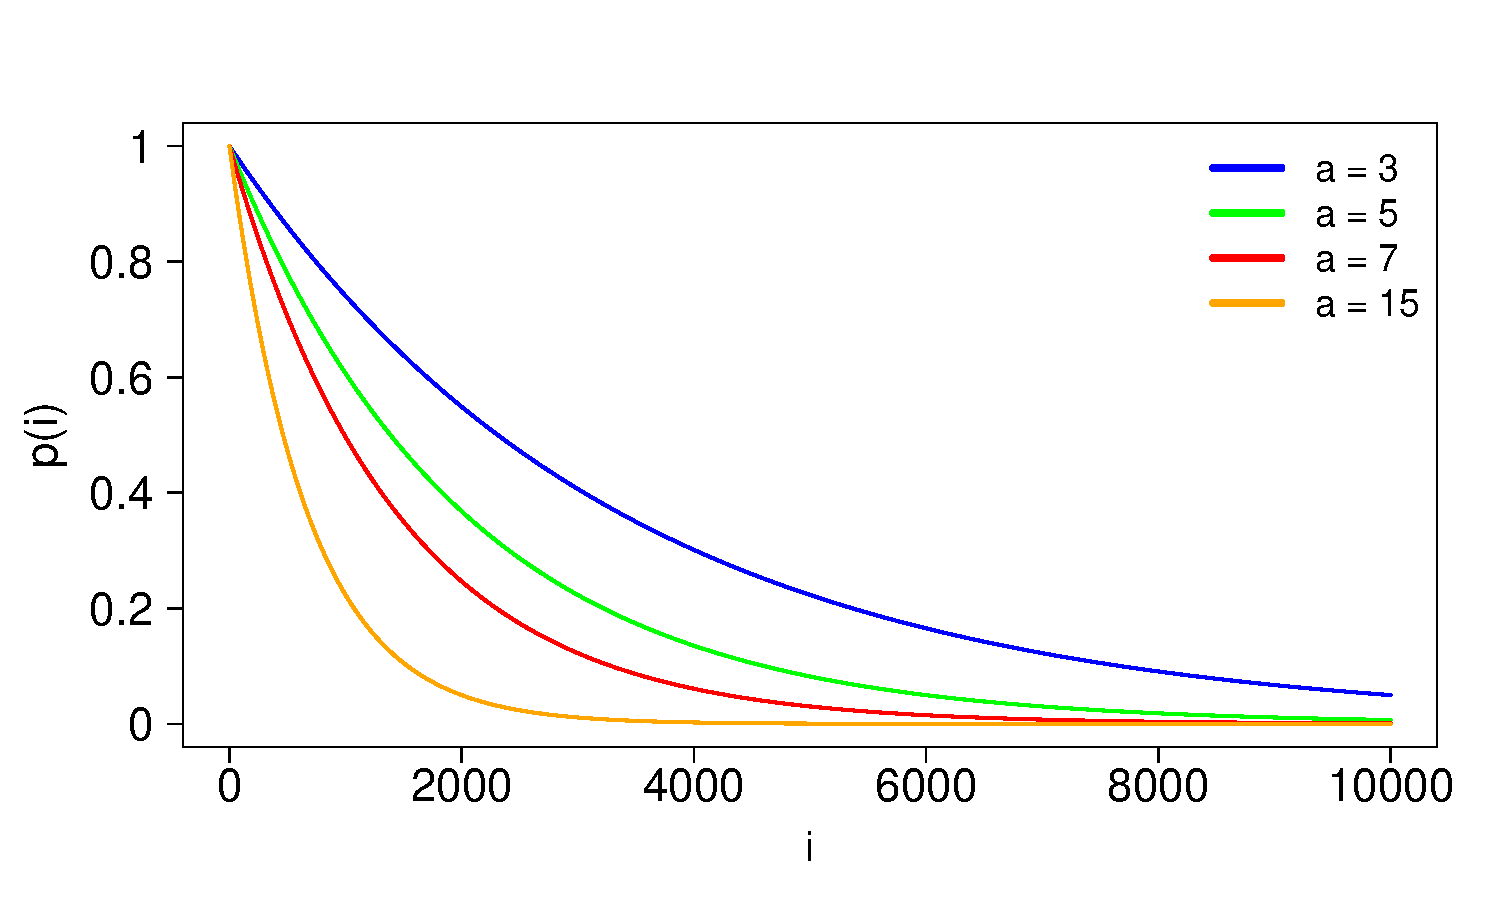
\includegraphics[width=2.8in]{exp_schedule_a.pdf}
	}
	\subfloat[$b=0.1$]{
	  \label{fig:exp_schedule_a_b}
		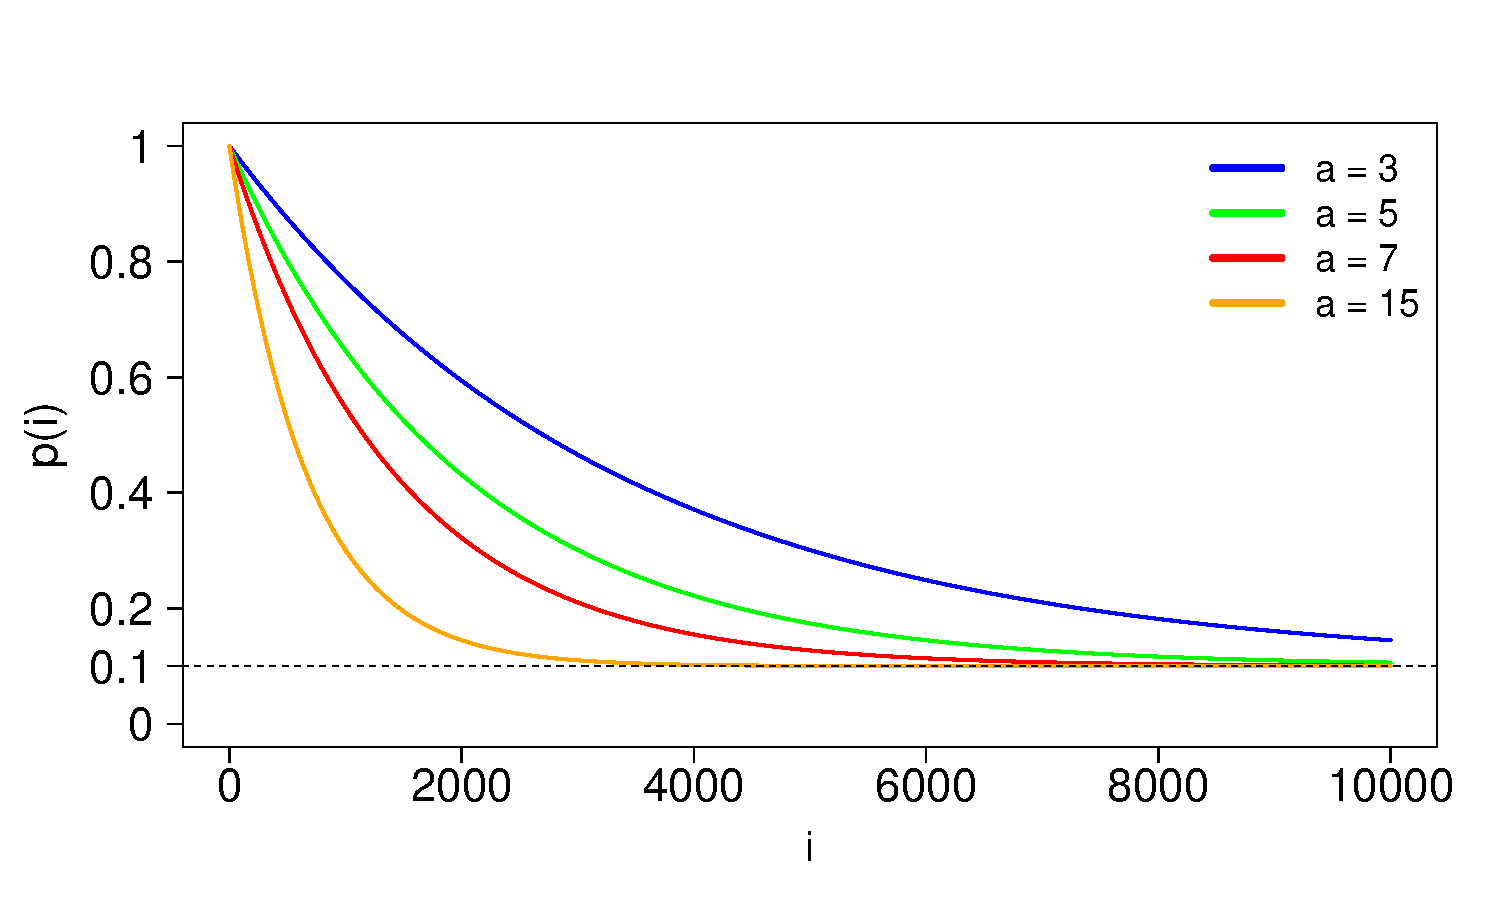
\includegraphics[width=2.8in]{exp_schedule_a_b.pdf}
	} \\
	\caption{Exponentially decaying schedule of probabilities $p(i)$ of making SMMALA proposals as a function of
	$i$-th MCMC iteration. The tuning factor $b$ sets the asymptotic probability of selecting the SMMALA proposal mechanism
	over its MALA counterpart. On the other hand, the tuning factor $a$ determines the rate of decay of $p(i)$ with larger 
	$a$ corresponding to more rapid decay.
	}
	\label{fig:exp_schedule}
\end{figure}

For other models, the curvature of the target density may change significantly over the region of parameter space with 
significant probability density. In such cases, rare updates to the metric after many iterations would lead to inefficient 
proposals. For such problems, it would be desirable to maintain a certain probability $b$ of making SMMALA proposals in late 
Monte Carlo iterations instead of eliminating this probability. Schedule \eqref{exp_schedule_a} can be modified as
\begin{equation}
\label{exp_schedule_a_b}
p(i)=(1-b)\exp{(-a(i-1)/n_m)}+b,
\end{equation}
where the additional tuning factor $b$ sets the asymptotic probability of using the SMMALA proposal mechanism in late MCMC
iterations. Obviously \eqref{exp_schedule_a} arises as a special case of \eqref{exp_schedule_a_b} by setting $b=0$ in the 
latter equation. Figure \ref{fig:exp_schedule_a_b} visualizes schedule \eqref{exp_schedule_a_b} for varying decaying rates 
and for $b=0.1$, which corresponds to a $10\%$ probability of picking SMMALA proposals as the simulation progresses towards 
its end.

A third and last question to be addressed in order to fully construct the hybrid sampler is how to set the preconditioning 
matrix for MALA proposals. Perhaps the simplest option would be to utlilize an identity preconditioning matrix $G=I$ 
corresponding to MALA proposal densities of the form
$\mathcal{N}(\boldsymbol{\theta}+\frac{\epsilon^2}{2}\nabla_{\theta}\log{p(\boldsymbol{\theta})}, \epsilon^2 I)$,
thus adhering to the most commonly used version of MALA. A more sophisticated algorithm is proposed in this paper that 
reuses the most recent metric $G(\boldsymbol{\theta}^0)$ computed at the latest state $\boldsymbol{\theta}^0$ obtained via a 
SMMALA update. This offers the benefits of making use of geometric information at no additional cost. The improvement in 
computational efficiency comes from caching and reusing $G(\boldsymbol{\theta}^0)$, $G^{-1}(\boldsymbol{\theta}^0)$ and 
$\sqrt{G^{-1}(\boldsymbol{\theta}^0)}$ for the intervening MALA steps between successive SMMALA updates. 

The resulting algorithm is abbreviated as ALSMMALA. The AL prefix implies that the bulk of states are drawn from a MALA 
proposal mechanism and the SMMALA suffix indicates that the local geometry is exploited via more expensive SMMALA updates.
Algorithm \ref{alsmmala} provides pseudocode to summarize ALSMMALA for some schedule $p(i)$.

\begin{algorithm}[t]
	\caption{ALSMMALA}
	\label{alsmmala}
	\begin{algorithmic}
		\State $\boldsymbol{\theta}^{\circ}=\boldsymbol{\theta}$\\
		
		\For{$k = 1$ to $n_m$} % \Comment{$n$: number of iterations}
		\State Sample $b \sim \mbox{Bernoulli}(p(i))$\\
		
		\State Sample $u\sim\mathcal{U}(0, 1)$\\
		
		\If {$b = 0$} \Comment{Use MALA proposal}
		\State Sample 
		$\boldsymbol{\theta^{*}}
		\sim\mathcal{N}(\boldsymbol{\mu}(\boldsymbol{\theta}, G(\boldsymbol{\theta}^{\circ}), \epsilon),
		\epsilon^2 G^{-1}(\boldsymbol{\theta}^{\circ}))
		$\\
		
		\If
		{
			$u<\dfrac{
				p(\boldsymbol{\theta}^{*})
				\mathcal{N}(\boldsymbol{\theta}|
					\boldsymbol{\mu}(\boldsymbol{\theta}^{*},
					G(\boldsymbol{\theta}^{\circ}),
					\epsilon),
					\epsilon^2 G^{-1}(\boldsymbol{\theta}^{\circ}))
			}
			{
				p(\boldsymbol{\theta})
				\mathcal{N}(\boldsymbol{\theta}^{*}|
					\boldsymbol{\mu}(\boldsymbol{\theta},
					G(\boldsymbol{\theta}^{\circ}),
					\epsilon),
					\epsilon^2 G^{-1}(\boldsymbol{\theta}^{\circ}))
			}$
		}
		
		\State $\boldsymbol{\theta}=\boldsymbol{\theta}^{*}$
		\EndIf
		\ElsIf {$b=1$} \Comment{Use SMMALA proposal}
		\State Sample 
		$\boldsymbol{\theta^{*}}
		\sim\mathcal{N}(\boldsymbol{\mu}(\boldsymbol{\theta}, G(\boldsymbol{\theta}), \epsilon),
		\epsilon^2 G^{-1}(\boldsymbol{\theta}))
		$\\
		
		\If
		{
			$u<\dfrac{
				p(\boldsymbol{\theta}^{*})
				\mathcal{N}(\boldsymbol{\theta}|
					\boldsymbol{\mu}(\boldsymbol{\theta}^{*},
					G(\boldsymbol{\theta}^{*}),
					\epsilon),
					\epsilon^2 G^{-1}(\boldsymbol{\theta}^{*}))
			}
			{
				p(\boldsymbol{\theta})
				\mathcal{N}(\boldsymbol{\theta}^{*}|
					\boldsymbol{\mu}(\boldsymbol{\theta},
					G(\boldsymbol{\theta}),
					\epsilon),
					\epsilon^2 G^{-1}(\boldsymbol{\theta}))
			}$
		}
		
		\State $\boldsymbol{\theta}=\boldsymbol{\theta}^{*}$
		\EndIf\\
		
		\State $\boldsymbol{\theta^{\circ}}=\boldsymbol{\theta}$
		\EndIf
		
		\EndFor
	\end{algorithmic}
\end{algorithm}

\subsection{Partial Manifold Langevin Metric Updates in Adaptive Metropolis}

The focal idea of this paper extends beyond ALSMMALA. In principle, it is suggested to allow the proposal mechanism to vary
between MCMC iterations. For example, most states can be sampled from a cheaper candidate-generating kernel, whereas fewer 
states can be drawn from a more costly proposal that uses local geometric information.

The candidate-generating kernel that contributes the majority of states to
% a chain simulated from
a hybrid sampler with a dual proposal mechanism impacts the statistical properties of the sampler.
For instance, \cite{rob_twe__exp} and \cite{liv_gir__inf} have shown that if a target density has tails heavier than 
exponential or lighter than Gaussian, then a MALA proposal kernel does not yield a geometrically ergodic Markov chain. For 
targets with such tail behaviour, ALSMMALA is not anticipated to admit geometric ergodicity either.

Depending on the target density, different proposal mechanisms might need to be combined to attain a hybrid sampler with
the desired statistical properties and sampling efficiency. In order to define a viable complement to ALSMMALA
and to further explore how to combine heterogeneous proposal mechanisms under a single MCMC algorithm, one more 
hybrid sampler with partial geometric updates will be constructed.

The new algorithm will sample most of its states from a proposal kernel inspired by the adaptive Metropolis (AM) kernel of
\cite{haa_sak_tam__ana}, while it will draw fewer states from the SMMALA proposal kernel. Given its candidate-generating
constituents, the new algorithm will be called AMSMMALA. The examples of Section \ref{Examples} will demonstrate the
relative performance of ALSMMALA and AMSMMALA for different target densities.

Initially, a concise account of the adaptive Metropolis algorithm of \cite{haa_sak_tam__ana} is given. Consider a hitherto
simulated chain $(\boldsymbol{\theta}_{0}, \boldsymbol{\theta}_{1},\dots,\boldsymbol{\theta}_{k})$, denoted by 
$\boldsymbol{\theta}_{0:k}$. It is noted that $\boldsymbol{\theta}_{i}\in\mathbb{R}^{n_{\theta}}$ refers to the $i$-th 
$n_{\theta}$-dimensional state of the chain, to 
be distinguished from the parenthesized subscript $\boldsymbol{\theta}_{(i)}\in\mathbb{R}$, which represents the $i$-th 
scalar coordinate of some state $\boldsymbol{\theta}\in\mathbb{R}^{n_{\theta}}$. A candidate state 
$\boldsymbol{\theta}^{\star}$ is sampled from the normal density
$\mathcal{N}(\boldsymbol{\theta}_{k}, \hat{C}(\boldsymbol{\theta}_{k}|\boldsymbol{\theta}_{0:k-1}))$. This proposal density 
is commonly centred on the last state $\boldsymbol{\theta}_{k}$ and its covariance matrix 
$\mbox{Cov}(\boldsymbol{\theta}_{k})$ is estimated adaptively by
\begin{equation}
\label{am_c}
\hat{C}(\boldsymbol{\theta}_{k}|\boldsymbol{\theta}_{0:k-1})=
s_{n_{\theta}}\widehat{\mbox{Cov}}(\boldsymbol{\theta}_{k}|\boldsymbol{\theta}_{0:k-1})+
s_{n_{\theta}}\lambda I,
\end{equation}
where $\widehat{\mbox{Cov}}(\boldsymbol{\theta}_{k}|\boldsymbol{\theta}_{0:k-1})$ is the empirical covariance 
matrix
\begin{equation}
\label{am_cov}
\widehat{\mbox{Cov}}(\boldsymbol{\theta}_{k}|\boldsymbol{\theta}_{0:k-1})=
\frac{1}{k-1}\left(
\sum_{i=0}^{k-1}\boldsymbol{\theta}_{i}\boldsymbol{\theta}_{i}^{T}-
k\bar{\boldsymbol{\theta}}_{k-1}\bar{\boldsymbol{\theta}}_{k-1}^{T}
\right).
\end{equation}
$\bar{\boldsymbol{\theta}}_{k-1}$ denotes the sample mean of $\boldsymbol{\theta}_{0:k-1}$. The tuning parameter 
$s_{n_{\theta}}$ depends only on the dimension $n_{\theta}$ of the parameter space and is used for scaling the empirical 
covariance. Furthermore, $\lambda>0$ is another tuning constant, which is chosen to be very small and is needed for 
preventing the estimator $\hat{C}(\boldsymbol{\theta}_{k}|\boldsymbol{\theta}_{0:k-1})$ from becoming degenerate for larger 
$k$. The candidate state $\boldsymbol{\theta}^{\star}$ is accepted with probability
\begin{equation}
\label{am_acceptance}
a(\boldsymbol{\theta}_{k},\boldsymbol{\theta}^{\star}) =
\min\left\{
\frac{p(\boldsymbol{\theta}^{\star})}{p(\boldsymbol{\theta}_{k})}
, 1
\right\}.
\end{equation}
Since the proposal kernel
$
\mathcal{N}(\boldsymbol{\theta}^{\star}|\boldsymbol{\theta}_{k}, 
\hat{C}(\boldsymbol{\theta}_{k}|\boldsymbol{\theta}_{0:k-1}))
$
is symmetric, it does not appear in the acceptance ratio \eqref{am_acceptance}.

To enable switching betweeen AM and SMMALA transitions, the covariance matrices of the two involved proposals must be brought
together under a common framework. If a SMMALA proposal $\boldsymbol{\theta}^{\star}$ is made at the $k$-th MCMC iteration, 
the local covariance at the current state $\boldsymbol{\theta}_k$ is evaluated exactly as
$\mbox{Cov}(\boldsymbol{\theta}_{k})=\epsilon^2 G^{-1}(\boldsymbol{\theta}_{k})$. If on the other hand a state 
$\boldsymbol{\theta}^{\star}$ is proposed via adjusted Metropolis at the $k$-th iteration, the metric 
$G(\boldsymbol{\theta}_{k})$ at the current state $\boldsymbol{\theta}_k$ may or may not be known depending on whether a
SMMALA or AM step was taken at the previous iteration; if a SMMALA step was taken at the previous iteration, then 
$G^{-1}(\boldsymbol{\theta}_{k})$ is available, otherwise an empirical estimator
$\widehat{G^{-1}}(\boldsymbol{\theta}_{k}|\boldsymbol{\theta}_{0:k-1})$ of $G^{-1}(\boldsymbol{\theta}_{k})$ must be 
obtained. Setting the diffusion drift step $\epsilon$ temporarily aside, it becomes clear that 
$G^{-1}(\boldsymbol{\theta}_{k})$ is either evaluated exactly by SMMALA or it is estimated by the empirical covariance
$
\widehat{G^{-1}}(\boldsymbol{\theta}_{k}|\boldsymbol{\theta}_{0:k-1})=
\widehat{\mbox{Cov}}(\boldsymbol{\theta}_{k}|\boldsymbol{\theta}_{0:k-1})
$
as given by \eqref{am_cov}.

As long as SMMALA steps are embedded throughout the AMSMMALA simulation, the AM estimator
$\widehat{G^{-1}}(\boldsymbol{\theta}_{k}|\boldsymbol{\theta}_{0:k-1})$ is corrected regularly by SMMALA exact inverse 
metric evaluations. Put another way, recurring geometric updates prevent the empirical covariance of
AM from becoming degenerate. Hence, the $s_{n_{\theta}}\lambda I$ term in \eqref{am_c} is omitted by setting $\lambda=0$.
Moreover, the tuning parameter $s_{n_{\theta}}$ of AM is set to $s_{n_{\theta}}=\epsilon^2$ in \eqref{am_c} so that
$\widehat{G^{-1}}(\boldsymbol{\theta}_{k}|\boldsymbol{\theta}_{0:k-1})$ and $G^{-1}(\boldsymbol{\theta}_k)$ are coherently
scaled by the same factor in AM and SMMALA updates respectively. Setting $\lambda=0$ and $s_{n_{\theta}}=\epsilon^2$ in
\eqref{am_c} defines the empirical covariance estimator
$\hat{C}(\boldsymbol{\theta}_{k}|\boldsymbol{\theta}_{0:k-1})=
\epsilon^2\widehat{G^{-1}}(\boldsymbol{\theta}_{k}|\boldsymbol{\theta}_{0:k-1})$
for the AM proposal density at the $k$-th step of AMSMMALA, where
$\widehat{G^{-1}}(\boldsymbol{\theta}_{k}|\boldsymbol{\theta}_{0:k-1})$ is given by \eqref{am_cov}.

To ensure that the adaptive Metropolis covariance estimator receives exact geometric updates regularly, a $\mod{(a)}$ 
scheduler can be employed. If the $k$-th MCMC iteration is a multiple of a tuning constant $a$, then a SMMALA update is 
attempted, else an AM proposal is made.

It follows from \eqref{am_cov} that the empirical inverse metric
$\widehat{G^{-1}}(\boldsymbol{\theta}_{k}|\boldsymbol{\theta}_{0:k-1})$, shortly denoted as
$\widehat{G^{-1}}(\boldsymbol{\theta}_{k})$, at the $k$-th AMSMMALA iteration calculates recursively as
\begin{equation}
\label{amsmmala_gm1}
(k-1)\widehat{G^{-1}}(\boldsymbol{\theta}_{k})=
(k-2)M(\boldsymbol{\theta}_{k-1})+
\boldsymbol{\theta}_{k-1} \boldsymbol{\theta}_{k-1}^{T}-
k\bar{\boldsymbol{\theta}}_{k-1} \bar{\boldsymbol{\theta}}_{k-1}^{T}+
(k-1)\bar{\boldsymbol{\theta}}_{k-2} \bar{\boldsymbol{\theta}}_{k-2}^{T}.
\end{equation}
The sample means in \eqref{amsmmala_gm1} are also calculable recursively according to
\begin{equation}
\label{amsmmala_mean_rec}
k\bar{\boldsymbol{\theta}}_k=(k-1)\bar{\boldsymbol{\theta}}_{k-1}+\boldsymbol{\theta}_k.
\end{equation}
Apparently, \eqref{amsmmala_gm1} and \eqref{amsmmala_mean_rec} help compute the empirical covariance of AMSMMALA faster than 
relying on \eqref{am_cov}.

The AM proposal kernel $\mathcal{N}(\boldsymbol{\theta}_{k}, \epsilon^2M(\boldsymbol{\theta}_{k}))$ at the 
$k$-th iteration of AMSMMALA has covariance that is either known exactly from the previous 
SMMALA step or it is estimated from the previous AM step, therefore
\begin{equation}
M(\boldsymbol{\theta}_{k})=
\left\{
\begin{array}{ll}
G^{-1}(\boldsymbol{\theta}_k), & \mbox{if $k-1$ step taken by SMMALA}\\
\widehat{G^{-1}}(\boldsymbol{\theta}_{k}), & \mbox{if $k-1$ step taken by AM}
\end{array}.
\right.
\end{equation}

Algorithm \ref{amsmmala} summarizes AMSMMALA with the help of pseudocode. The empirical covariance 
$\widehat{G^{-1}}(\boldsymbol{\theta}_{k})$ in Algorithm \ref{amsmmala} is computed via \eqref{amsmmala_gm1}.

\begin{algorithm}[t]
	\caption{AMSMMALA}
	\label{amsmmala}
	\begin{algorithmic}
		\For{$k = 1$ to $n_m$} % \Comment{$n$: number of iterations}
		% \State Sample $b \sim \mbox{Bernoulli}(p(i))$
		\If {$k \equiv 0~(\mod{(a)})$}
		\State $b_k = 1$
		\Else
		\State $b_k = 0$
		\EndIf\\
		
		\State Sample $u\sim\mathcal{U}(0, 1)$\\
		
		\If {$b_k = 0$} \Comment{Use adaptive Metropolis proposal}
		\If {$b_{k-1}=1$}
		\State $M(\boldsymbol{\theta}_k)=G^{-1}(\boldsymbol{\theta}_k)$
		\ElsIf {$b_{k-1}=0$}
		\State $M(\boldsymbol{\theta}_k)=\widehat{G^{-1}}(\boldsymbol{\theta}_{k})$
		\EndIf\\

		\State Sample 
		$\boldsymbol{\theta^{*}}
		\sim\mathcal{N}(\boldsymbol{\theta}_k,
		\epsilon^2 M(\boldsymbol{\theta}_k)) %\widehat{G^{-1}}(\boldsymbol{\theta}|\boldsymbol{\theta}_{0:k-1}))
		$\\
		
		\State $r = \dfrac{p(\boldsymbol{\theta}^{*})}{p(\boldsymbol{\theta}_k)}$
		\ElsIf {$b_k=1$} \Comment{Use SMMALA proposal}
		\State Sample 
		$\boldsymbol{\theta^{*}}
		\sim\mathcal{N}(\boldsymbol{\mu}(\boldsymbol{\theta}_k, G(\boldsymbol{\theta}_k), \epsilon),
		\epsilon^2 G^{-1}(\boldsymbol{\theta}_k))
		$\\

		\State $r = \dfrac{
				p(\boldsymbol{\theta}^{*})
				\mathcal{N}(\boldsymbol{\theta}_k|
				\boldsymbol{\mu}(\boldsymbol{\theta}^{*},
				G(\boldsymbol{\theta}^{*}),
				\epsilon),
				\epsilon^2 G^{-1}(\boldsymbol{\theta}^{*}))
			}
			{
				p(\boldsymbol{\theta}_k)
				\mathcal{N}(\boldsymbol{\theta}^{*}|
				\boldsymbol{\mu}(\boldsymbol{\theta}_k,
				G(\boldsymbol{\theta}_k),
				\epsilon),
				\epsilon^2 G^{-1}(\boldsymbol{\theta}_k))
			}$
		\EndIf\\

		\If
		{
			$u<r$
		}
		  \State $\boldsymbol{\theta}_{k+1}=\boldsymbol{\theta}^{*}$
		\Else
		  \State $\boldsymbol{\theta}_{k+1}=\boldsymbol{\theta}_k$		
		\EndIf
		
		\EndFor
	\end{algorithmic}
\end{algorithm}

The AM steps of AMSMMALA waive the cost of proposal evaluations thanks to the acceptance probability \eqref{am_acceptance}
and do not require computing log-target derivatives. However, sampling a candidate state from the AM proposal kernel creates
a complexity bottleneck of $\mathcal{O}(n_{\theta}^3)$ due to the associated Cholesky decomposition of the empirical 
covariance. The recursive formula \eqref{amsmmala_gm1} comes to rescue, as it allows to replace the Cholesky factorization 
by two rank one updates and one rank one downdate, thus reducing the complexity of AM updates from 
$\mathcal{O}(n_{\theta}^3)$ to $\mathcal{O}(3n_{\theta}^2)$. \cite{gill_gol_wal__met} and \cite{see__low} elaborate on low 
rank updates for Cholesky decompositions.

AMSMMALA yields two more advantages over AM apart from exploiting local geometric information. An initial covariance matrix
$\hat{C}_0=\epsilon^2\widehat{G^{-1}}(\boldsymbol{\theta}_{0})$ is needed for starting up the recursion in
\eqref{amsmmala_gm1}. \cite{haa_sak_tam__ana} propose to choose $\hat{C}_0$ on the basis of prior knowledge. If prior 
elicitation for $\hat{C}_0$ turns to be non-trivial, AMSMMALA gives the option to initialize $C_0=\epsilon^2 
G^{-1}(\boldsymbol{\theta}_{0})$ by a SMMALA update. Additionally, the recurring corrections of the empirical covariance via 
exact SMMALA updates make AMSMMALA available to target densities of non-bounded support, extending this way the range of 
applicability of the original AM algorithm by \cite{haa_sak_tam__ana}. 

\subsection{Choice of Update Schedule}

The two proposal mechanisms along with the schedule for picking between them comprise the three main building blocks of any
resulting hybrid sampler. ALSMMALA and AMSMMALA have manifested ways of combining cheap with more expensive geometric updates
to construct a new MCMC algorithm. The underlying proposals set some limitations in the choice of schedule. AMSMMALA for
example needs to receive exact metric updates throughout the course of simulation to correct the empirical covariance used in
adaptive Metropolis steps. Despite any inherent limitations posed by the proposal mechanisms, there is room for 
experimentation when choosing a schedule.

For instance, a geometric distribution $\mbox{Geometric}(p)$ could be used for regulating the occurrence of metric updates 
in AMSMMALA, where $p$ is a tuning parameter giving the probability of making a SMMALA proposal. Setting $p=1/(1+a)$ yields 
an expected number of $(1-p)/p=a$ AM steps before a new SMMALA proposal is made. This way, the $\mbox{Geometric}(1/(1+a))$ 
schedule is a stochastic analogue to the deterministic $\mod{(a)}$ schedule of Algorithm \ref{amsmmala}.

Other samplers with dual proposal mechanism, such as ALSMMALA, do not need regular geometric steps, thence it makes sense to 
exploit local geometric information mostly in the early transient phases of the simulated chain and to reduce computational 
load via a cheaper proposal in late stationary phases. A $\mbox{Bernoulli(p(i))}$ distribution comes in handy, leaving space 
for experimentation with the choice of schedule for $p(i)$. The probability $p(i)$ plays a role analogous to temperature in 
the cooling schedule of simulated annealing. This analogy brings up a prolific body of literature to open up possibilities 
for scheduling the cooling of probability $p(i)$ of geometric updates.

Table \ref{tab:cooling_schedules} suggests four cooling schedules for $p(i)$, which have been acquired empirically and are 
variants of temperature schedules previously discussed by \cite{haj__coo} and \cite{nou_and__aco}.
Figure \ref{fig:cooling_schedules} displays instances of the four schedules of Table \ref{tab:cooling_schedules}.

\begin{table}[t]
\centering
\begin{tabular}{l|c}
\hline\noalign{\smallskip}
Cooling & $p(i)$\\
\noalign{\smallskip}\hline\noalign{\smallskip}
Exponential & $(1-b)\exp(-a(i-1)/n_m)+b$\\
\noalign{\smallskip}\hline\noalign{\smallskip}
Linear & $\dfrac{1-b}{1+a(i-1)/n_m}+b$\\
\noalign{\smallskip}\hline\noalign{\smallskip}
Quadratic & $\dfrac{1-b}{1+a((i-1)/n_m)^2}+b$\\
\noalign{\smallskip}\hline\noalign{\smallskip}
Logarithmic & $\dfrac{(1-b)}{1+a\log(1+(i-1)/n_m)}+b$\\
\noalign{\smallskip}\hline
\end{tabular}
\caption{
Different types of cooling schedule for probability $p(i),~i\in\left\{1,2,\dots,n_m\right\}$, of making a geometric proposal 
as a function of the $i$-th MCMC iteration. Such cooling for $p(i)$ is plausible if the dual proposal scheme does not 
require regular geometric updates throughout the simulation.
}
\label{tab:cooling_schedules}
\end{table}

\begin{figure}[t]
\centering
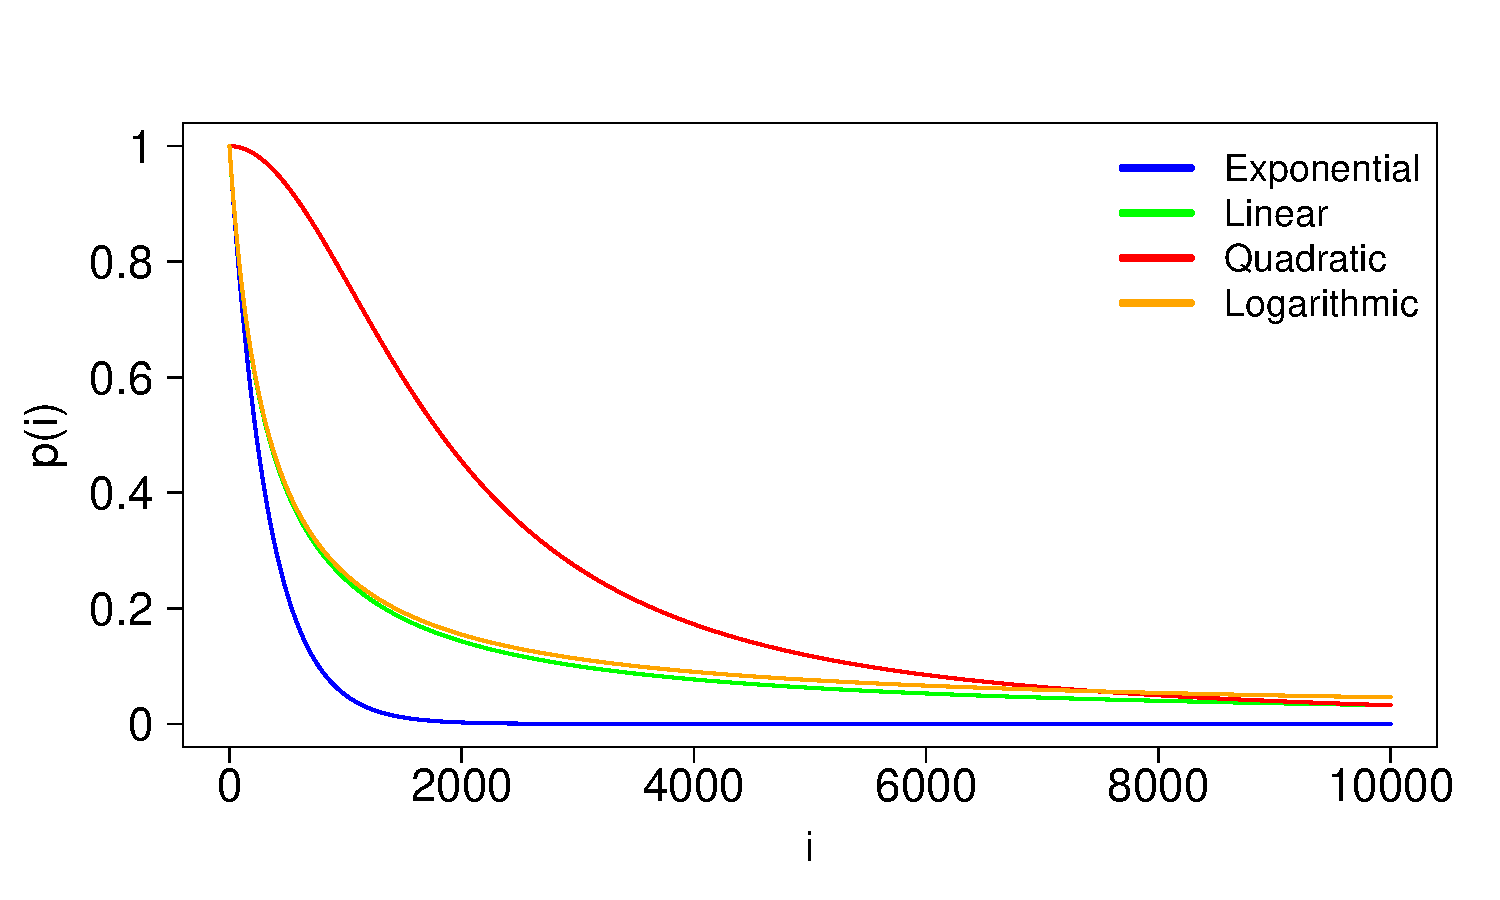
\includegraphics[width=2.8in]{cooling_schedules.pdf}
\caption{
Visualization of four cooling schedule types of Table \ref{tab:cooling_schedules} for probability $p(i)$ of making a 
geometric proposal as a function of the $i$-th MCMC iteration. The displayed schedules have been generated using $a=30$ and 
$b=0$.
}
\label{fig:cooling_schedules}
\end{figure}

\subsection{Expected Complexity}
\label{Expected Complexity}

The concept of complexity carries three distinct meanings in the context of MCMC. Firstly, MCMC methods need to be tuned so
as to achieve a balance between proposing large enough jumps and ensuring that a reasonable proportion of jumps are accepted.
By way of illustration, MALA attains its optimal acceptance rate of $0.574$ as $n_{\theta}\rightarrow\infty$ by setting its
drift step $\epsilon$ to be in the vicinity of $n_{\theta}^{-1/3}$. Because of this, it is said that the algorithmic
efficiency of MALA scales $\mathcal{O}(n_{\theta}^{-1/3})$ as the number $n_{\theta}$ of parameters increases.

Secondly, the quality of MCMC algorithms is assessed by estimating the effective sample size (ESS) of their simulated chains.
The ESS of a chain is interpreted as the number of samples in the chain bearing the same amount of variance as the one found 
in $n_m$ independent samples.

A third criterion for assessing MCMC methods is their computational time.
This criterion corresponds to the ordinary concept of algorithmic complexity as it entails a count of numerical operations
performed by an MCMC algorithm. To give an example, the computational complexity of MALA with an identity preconditioning
matrix is of order $\mathcal{O}(n_{\theta})$, as explained in Section \ref{Motivation}.

Of these three indicators of algorithmic complexity, ESS and computational runtime are the ones typically used for
understanding the range of applicability of MCMC methods. To get a single-number summary, the ratio of ESS over runtime is
usually employed. In the present paper, the computational time of ALSMMALA and AMSMMALA are derived theoretically for models
whose complexity do not dominate the computations (as discussed in Section \ref{Motivation}), while both samplers are 
empirically assessed in Section \ref{Examples} via their ESS and CPU runtime.

\begin{proposition}
Let $A_1$ and $A_2$ be two MCMC algorithms whose proposal mechanisms have computational complexities $c_1$ and $c_2$, 
respectively. A composite MCMC algorithm $A$ conducts a Bernoulli trial
$B(i)\sim\mbox{Bernoulli}(p(i))~,i\in\left\{1,2,\dots,n_m\right\}$, to take its $i$-th step using the proposal kernel of 
algorithm $A_1$ with probability $p(i)$, or using the proposal mechanism of $A_2$ with probability $1-p(i)$. The mean 
complexity of $A$ is given by
\begin{equation}
\label{eq:c}
\mathcal{O}\left(
\dfrac{\sum_{i=1}^{n_m}p(i)}{n_m}c_1+\dfrac{n_m-\sum_{i=1}^{n_m}p(i)}{n_m}c_2
\right).
\end{equation}
\end{proposition}

\begin{proof}
The expected number of invocations of the proposal kernel associated with algorithm $A_1$ equals 
\begin{equation*}
E\left(\sum_{i=1}^{n_m}B(i)\right)=\sum_{i=1}^{n_m}E(B(i))=\sum_{i=1}^{n_m}p(i),
\end{equation*}
whence the conclusion follows directly.
\end{proof}

\begin{proposition}
If an exponentially decaying schedule $p(i)$, as described by \eqref{exp_schedule_a}, is used for regulating the choice of 
proposal kernel at each step of algorithm $A$, then the expected complexity of $A$ becomes
\begin{equation}
\label{eq:c_exp}
\mathcal{O}\left(
\dfrac{1-\exp{(-a)}}{n_m(1-\exp{(-a/n_m)})}c_1+
\left(1-\dfrac{1-\exp{(-a)}}{n_m(1-\exp{(-a/n_m)})}\right)c_2
\right).
\end{equation}
\end{proposition}

\begin{proof}
Schedule \eqref{exp_schedule_a} yields the geometric series sum
\begin{equation}
\label{eq:c_exp_geom}
\sum_{i=1}^{n_m}p(i)=
\sum_{i=1}^{n_m}\exp{(-a(i-1)/n_m)}=
\dfrac{1-\exp{(-a)}}{1-\exp{(-a/n_m)}}.
\end{equation}
Plugging \eqref{eq:c_exp_geom} into \eqref{eq:c} gives \eqref{eq:c_exp}.
\end{proof}

\begin{lemma}
For sufficiently large number $n_m$ of MCMC iterations ($n_m\rightarrow\infty$), the mean complexity of an algorithm $A$ 
with exponentially decaying schedule \eqref{exp_schedule_a} is.
\begin{equation}
\label{eq:c_exp_limit}
\mathcal{O}\left(
\dfrac{1-\exp{(-a)}}{a}c_1+
\left(1-\dfrac{1-\exp{(-a)}}{a}\right)c_2
\right).
\end{equation}
\end{lemma}

\begin{proof}
It suffices to notice that
\begin{equation}
\lim_{n_m\to\infty}\dfrac{1-\exp{(-a)}}{n_m(1-\exp{(-a/n_m)})}=\dfrac{1-\exp{(-a)}}{a}.
\end{equation}
\end{proof}

\begin{proposition}
The mean complexity of an algorithm $A$ with a $\mod{(a)}$ schedule $p(i)$ is
\begin{equation}
\label{eq:c_mod}
\mathcal{O}\left(
\dfrac{1}{a}c_1+
\dfrac{a-1}{a} c_2
\right).
\end{equation}
\end{proposition}

\begin{proof}
The proposal mechanism of algorithm $c_1$ is called $n_m/a$ times out of $n_m$ iterations. Hence, the proportion of proposals
made via $c_1$ is $1/a$, which completes the proof.
\end{proof}

\begin{lemma}
For a large number $n_m$ of iterations ($n_m\rightarrow\infty$), the expected complexity of ALSMMALA, as presented in 
Algorithm \ref{alsmmala} and equipped with the exponentially decaying schedule defined by \eqref{exp_schedule_a}, is given by
\begin{equation}
\label{eq:c_alsmmala_exp}
\mathcal{O}\left(
\dfrac{1-\exp{(-a)}}{a}n_{\theta}^3+
\left(1-\dfrac{1-\exp{(-a)}}{a}\right)n_{\theta}^2
\right).
\end{equation}
\end{lemma}

\begin{proof}
\eqref{eq:c_alsmmala_exp} follows from \eqref{eq:c_exp_limit} by recalling that the respective complexities of SMMALA and 
MALA are $\mathcal{O}(n_{\theta}^3)$ and $\mathcal{O}(n_{\theta}^2)$.
\end{proof}

\begin{lemma}
The expected complexity of AMSMMALA, as defined in Algorithm \ref{amsmmala}, is
\begin{equation}
\label{eq:c_amsmmala_mod}
\mathcal{O}\left(
\dfrac{1}{a}n_{\theta}^3+
\dfrac{a-1}{a}n_{\theta}^2
\right).
\end{equation}
\end{lemma}

\begin{proof}
Setting $c1=n_{\theta}^3$ and $c_2=n_{\theta}^2$ in \eqref{eq:c_mod}, which correspond to the complexity orders of SMMALA 
and AM, gives \eqref{eq:c_amsmmala_mod}.
\end{proof}

The schedule $p(i)$ for choosing between proposal mechanisms plays a decisive role in the complexity of the resulting sampler
as seen from \eqref{eq:c}. Besides, the decaying rate $a$ of an exponentially decaying schedule \eqref{exp_schedule_a} and 
the modulus $a$ of a $\mod{(a)}$ schedule can be used for adjusting the computational cost according to 
\eqref{eq:c_exp_limit} and \eqref{eq:c_mod}.

Figure \ref{fig:alsmmala_amsmmala_schedule} displays the complexity of ALSMMALA with an exponential schedule specified by
\eqref{exp_schedule_a} and AMSMMALA with a $\mod{(a)}$ schedule as a function of the parameter space dimension $n_{\theta}$.
The curves of Figures \ref{fig:alsmmala_exp_schedule} and \ref{fig:amsmmala_mod_schedule} correspond to varying levels of 
decaying rate $a$ for ALSMMALA and of modulus $a$ for AMSMMALA. In both cases, the tuning factor $a$ determines the 
trade-off between runtime and amount of geometric computation. Larger values of $a$ reduce the runtime due to fewer 
geometric updates, whereas smaller values of $a$ increase the complexity as they induce more geometric updates.

\begin{figure}[t]
	\centering
	\subfloat[ALSMMALA]{
		\label{fig:alsmmala_exp_schedule}
		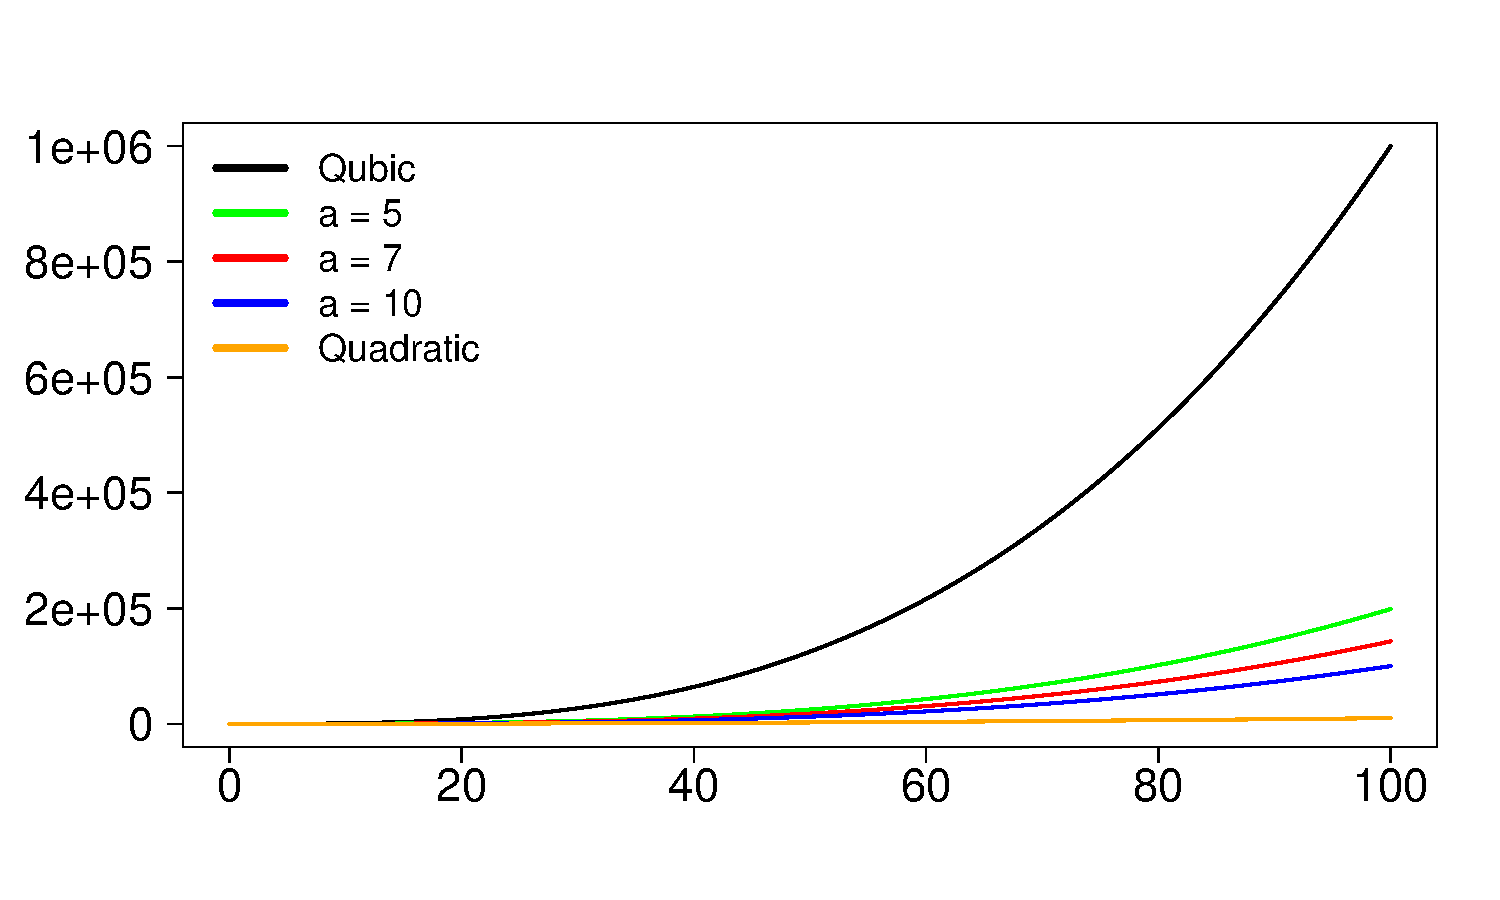
\includegraphics[width=2.8in]{alsmmala_complexity.pdf}
	}
	\subfloat[AMSMMALA]{
		\label{fig:amsmmala_mod_schedule}
		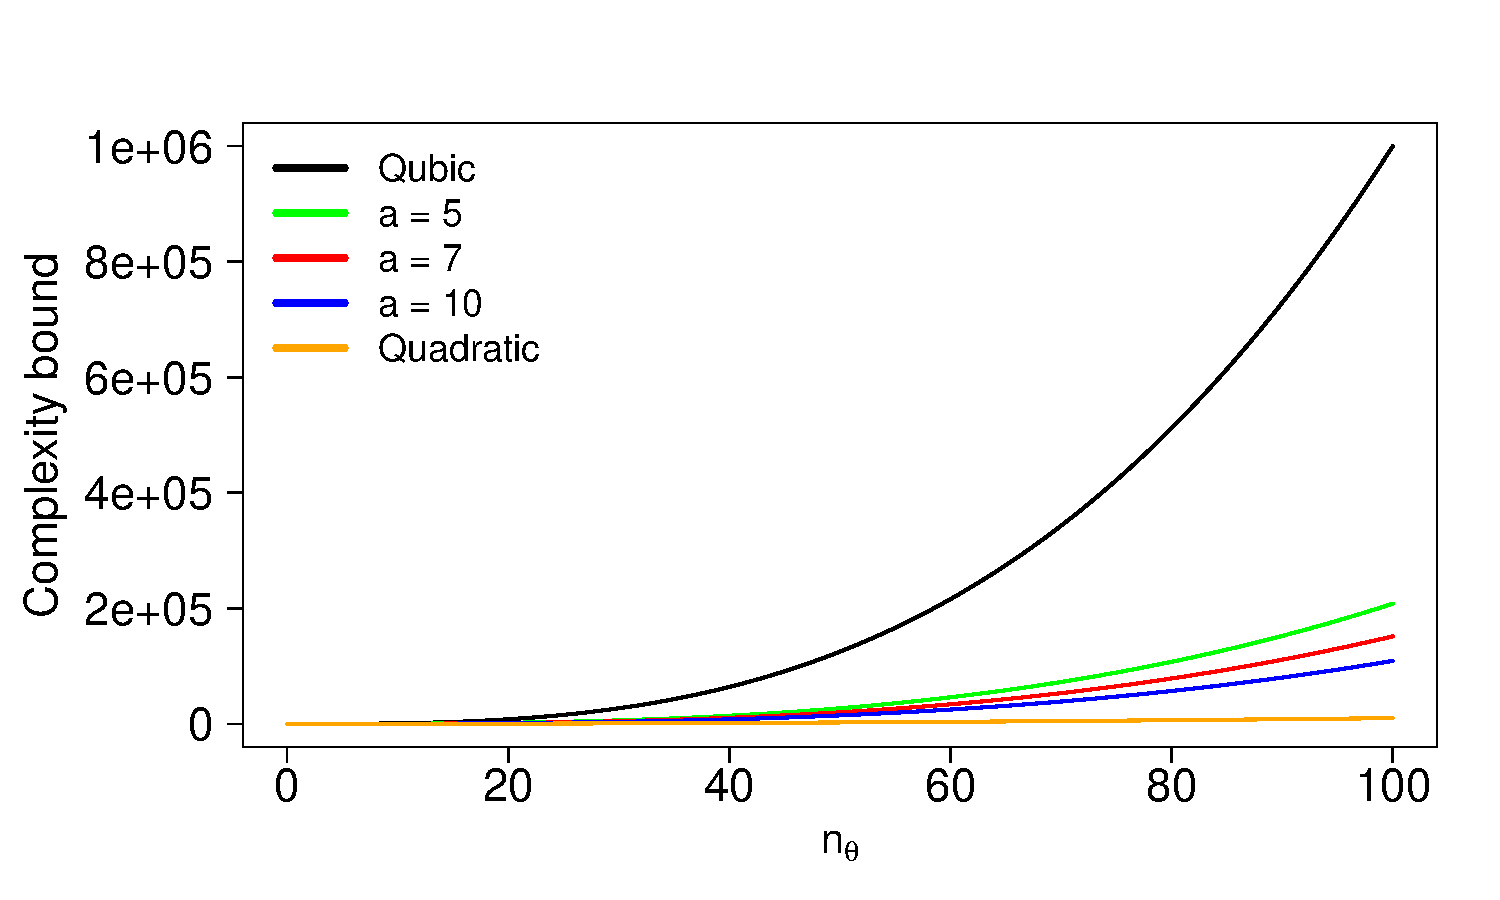
\includegraphics[width=2.8in]{amsmmala_complexity.pdf}
	} \\
	\caption{
		Time complexity of ALSMMALA with an exponential schedule given by \eqref{exp_schedule_a} and AMSMMALA with a $\mod{(a)}$ 
		schedule as a function of the number $n_{\theta}$ of parameters. Different curves correspond to varying levels of 
		decaying rate $a$ for ALSMMALA and of modulus $a$ for AMSMMALA. The cubic complexity of SMMALA and quadratic complexity
		of MALA with a preconditioning matrix other than the identity matrix are displayed as baseline cases.
	}
	\label{fig:alsmmala_amsmmala_schedule}
\end{figure}

\subsection{Analytically Intractable Geometric Updates}

In practice, challenges in the implementation of manifold MCMC algorithms might raise additional computational implications.
In particular, two notoriously recurring issues relate to the Cholesky decomposition of metric $G^{-1}(\boldsymbol{\theta})$ 
and to the calculation of up to third order derivatives of $G(\boldsymbol{\theta})$.

Various contributing factors, including finite-precision floating point arithmetic, can lead to an indefinite proposal
covariance matrix $\epsilon^2 G^{-1}(\boldsymbol{\theta})$. This in turn breaks the Cholesky factorization of 
$\epsilon^2 G^{-1}(\boldsymbol{\theta})$. \cite{bet__age} introduced the so-called SoftAbs metric, which offers a 
positive definite approximation of the indefinite proposal covariance. The working SoftAbs solution to the Cholesky 
factorization problem involves an eigen-decomposition, so it comes with an $\mathcal{O}(n_{\theta}^3)$ cost.
Other research avenues pursuit different positive definite approximations of indefinite matrices. The works of 
\cite{hig__com01} and \cite{hig__com02} for example approximate the nearest symmetric positive semi-definite matrix in the 
Frobenius norm to an arbitrary real matrix. If future research succeeds in adapting the approach of \cite{hig__com01} in the 
context of geometric MCMC methods, then a computationally cheaper alternative to the SoftAbs metric could become available.

Non-trivial models can render the analytic derivation of log-target derivatives impossible or impractical. Automatic
differentiation (AD), a computationally driven research activity that has evolved since the mid 1950's, helps compute 
derivatives in a numerically exact way. Indeed, \cite{gri__ona} has shown that AD is backward stable in the sense of 
\cite{wil__mod}. Thus, small perturbations of the original function due to machine precision still yield accurate 
derivatives calculated via AD.

There are different methods of automatic differentiation that mainly differ in the way they traverse the chain rule; reverse 
mode AD is better suited for functions $f:\mathbb{R}^n\rightarrow\mathbb{R}$, in contrast to forward mode AD that is more 
suitable for functions $f:\mathbb{R}\rightarrow\mathbb{R}^m$ (\cite{gri_wal__eva}). Consequently, reverse mode AD is 
utilized for computing derivatives of probability distributions, and finds use in statistical inference. Reverse mode AD is 
not worse than that of the respective analytical derivatives of a target density in terms of complexity, but it poses high
memory requirements. Hybrid AD procedures combining elements of forward and backward propagation of derivatives can be 
constructed for achieving a compromise between execution time and memory usage when differentiating functions of the form
$f:\mathbb{R}^n\rightarrow\mathbb{R}^m$.

\section{Example Applications}
\label{Examples}

ALSMMALA and AMSMMALA are put to test via three examples to empirically validate these two MCMC algorithms and to assess 
their computational efficacy. Ten chains are simulated from each sampler of each example. $110,000$ iterations are run for 
the realization of each chain, of which the first $10,000$ burn-in are discarded, so $n_m=100,000$ MCMC samples are retained.

The effective sample size (ESS) of each dimension $\boldsymbol{\theta}_{(i)},~i\in\left\{1,2,\dots,n_{\theta}\right\}$,
of the parameter vector $\boldsymbol{\theta}$ is computed as
\begin{equation}
\mbox{ESS} =
\dfrac{n_m\hat{\sigma}^2_{IID}}{\hat{\sigma}^2_{MCMC}},
\end{equation}
where $\hat{\sigma}^2_{IID}$ and $\hat{\sigma}^2_{MCMC}$ denote the ordinary and Monte Carlo variance of the associated 
chain. The Monte Carlo variance $\hat{\sigma}^2_{MCMC}$ is calculated by means of the initial monotone sequence estimator of
\cite{gey__pra}. To get more reliable estimates, the ESS of each dimension and the CPU runtime are averaged by taking their
respective means across every set of ten chains simulated from a sampler. The computational efficiency of each sampler is
defined as the ratio $\min\left\{\mbox{ESS}_i:i=1,2,\dots,n_{\theta}\right\}/\mbox{time}$ of the smallest ESS
$\min\left\{\mbox{ESS}_i:i=1,2,\dots,n_{\theta}\right\}$ among all $n_{\theta}$ dimensions over the simulation time. Finally,
the relative speed-up of one MCMC method over another is set to be the ratio of their computational efficiencies.

A package, called PGUManifoldMC, has been developed to implement ALSMMALA and AMSMMALA using the Julia programming language.
PGUManifoldMC is based on Lora, a package for MCMC inference written in Julia by one of the two authors. PGUManifoldMC is
publicly available at \url{https://github.com/scidom/PGUManifoldMC.jl} under an MIT license. The PGUManifoldMC package ships
with the three examples of this paper.

\subsection{Bayesian Logistic Regression}

As a first example, consider a Bayesian logistic regression model consisting of $n_d$ samples and $n_{\theta}$ covariates. 
The log-likelihood of the model expresses as
\begin{equation}
\label{eq:logit_logl}
L(\mathbf{y}, X | \boldsymbol{\theta})=
(X\boldsymbol{\theta})^T\mathbf{y}-
\sum_{i=1}^{n_d}\log\left(1+\exp(\boldsymbol{\theta}^T
\mathbf{x_{i,}})\right),
\end{equation}
where $y\in\{0,1\}^{n_d}$ is the binary response variable, $X$ the $n_d\cdot n_{\theta}$ design matrix, $\mathbf{x_{i,}}$ 
the $i$-th row of $X$ and $\boldsymbol{\theta}\in\mathbb{R}^{n_{\theta}}$ the regression coefficients. A normal prior is 
assumed for the model parameters $\boldsymbol{\theta}\sim\pi({\boldsymbol{\theta}})=\mathcal{N}(\boldsymbol{0},vI)$ for some
positive hyperparameter $v$. The unnormalized log-target density for Bayesian logistic regression thus takes the form
\begin{equation}
\label{eq:logit_target}
\log{(p(\boldsymbol{\theta}|\mathbf{y}, X))}=L(\mathbf{y}, X | \boldsymbol{\theta})+\log{(\pi(\boldsymbol{\theta}))},
\end{equation}
where the log-likelihood is given by \eqref{eq:logit_logl}.

Differentiating \eqref{eq:logit_logl} gives the gradient of the log-likelihood
\begin{equation}
\label{eq:logit_gradlogl}
\nabla_{\boldsymbol{\theta}}(L(\mathbf{y},X|\boldsymbol{\theta}))=
X^T\left(\mathbf{y}-
\frac{1}{1+\exp\left(-X\boldsymbol{\theta}\right)}\right).
\end{equation}
The gradient of the log-prior evaluates as
\begin{equation}
\label{eq:logit_gradlogprior}
\nabla_{\boldsymbol{\theta}}(\log{(\pi({\boldsymbol{\theta}}))})=
-\frac{1}{v}\boldsymbol{\theta}.
\end{equation}
So, the gradient
$\nabla_{\boldsymbol{\theta}}(\log{(p(\boldsymbol{\theta}|\mathbf{y}, X))})$ of the log-target equals the sum of
\eqref{eq:logit_gradlogl} and \eqref{eq:logit_gradlogprior}.

The metric of a log-target $\log{(p)}$ is conventionally taken to be the expected Fisher information of $\log{(p)}$, which 
is equal to the  negative Hessian of log-likelihood $L$ minus the Hessian of log-prior $\log{(\pi)}$ in a Bayesian setting. 
By differentiating 
\eqref{eq:logit_gradlogl} and \eqref{eq:logit_gradlogprior}, it is deduced that the metric 
$G(\boldsymbol{\theta}|X)$ for the Bayesian logistic regression model with a normal prior $\mathcal{N}(\boldsymbol{0},vI)$ is
\begin{equation}
\label{eq:blr:G:normalprior}
G(\boldsymbol{\theta}|X))=X^T\Lambda(\boldsymbol{\theta})X+
\frac{1}{v}I,
\end{equation}
where the $n_d\cdot n_d$ diagonal matrix $\Lambda(\boldsymbol{\theta})=\mbox{diag}\left[p_i(1-p_i)\right]$ has diagonal 
elements
\begin{equation}
p_i=P(y_i=1)=\exp(\boldsymbol{\theta}^T\mathbf{x_{i,}})/
(1+\exp(\boldsymbol{\theta}^T\mathbf{x_{i,}})),~i\in\left\{1,2,\dots,n_{d}\right\}.
\end{equation}

The gradient
$\nabla_{\boldsymbol{\theta}}(\log{(p(\boldsymbol{\theta}|\mathbf{y}, X))})$
of the Bayesian logistic log-target is needed for MALA proposals made by ALSMMALA. Both the log-target gradient
$\nabla_{\boldsymbol{\theta}}(\log{(p(\boldsymbol{\theta}|\mathbf{y}, X))})$ and metric
$G(\boldsymbol{\theta}|X))$ are needed for SMMALA proposals made by either of ALSMMALA and AMSMMALA.

MALA, SMMALA, ALSMMALA and AMSMMALA are run on the bank dataset taken from \cite{flu_rie__mul} with the Bayesian logistic 
regression log-target outlined in the current section and with the prior hyperparameter set to $v=100$, which implies a  
flat non-informative prior. The bank dataset contains the measurements of $n_{\theta}=4$ covariates on $n_d=200$ Swiss 
banknotes, $100$ of which are genuine and $100$ counterfeit. The four covariates include the length of the bill, the width 
of the left and right edge, and the bottom margin width. The binary response variable is the type of banknote, $0$ being 
genuine and $1$ counterfeit.

Table \ref{tab:logit} summarizes the sampling efficacy metrics for the Bayesian logistic example. MALA is taken as the 
baseline sampler in the speedup calculations. As expected, the effective sample size of SMMALA is higher across most of 
covariates in comparison to MALA. The relative advantage of SMMALA over MALA in terms of ESS is attributed to the fact that 
the former sampler exploits local geometric information via successive evaluations of metric $G(\boldsymbol{\theta})$. On 
the other hand, SMMALA is more than twice slower in comparison to MALA as the respective runtimes show. Overall, SMMALA
exhibits a slowdown factor of $0.73$ with respect to the MALA baseline. This is a demonstration of how the increased
sampling effectiveness of manifold MCMC algorithms is outweighed by their computational cost.

\begin{table}[t]
	\centering
	\begin{tabular}{l|r|rrrr|r|r|r}
		\hline\noalign{\smallskip}
		\multirow{2}{*}{Method} &
		\multirow{2}{*}{AR} &
		\multicolumn{4}{c|}{ESS} &
		\multirow{2}{*}{Time} &
		\multirow{2}{*}{Efficiency} &
		\multirow{2}{*}{Speedup} \\
		& & $\theta_1$ & $\theta_2$ & $\theta_3$ & $\theta_4$ & & & \\
		\noalign{\smallskip}\hline\noalign{\smallskip}
		MALA & .60 & 23077 & 8039 & 8892 & 8562 & 3.05 & 2637.47 & 1.00 \\
		SMMALA & .69 & 15138 & 15246 & 15098 & 12989 & 6.78 & 1916.05 & 0.73 \\
		AMSMMALA & .25 & 9114 & 9159 & 9147 & 8635 & 3.84 & 2246.86 & 0.85 \\
	  ALSMMALA & .63 & 31562 & 31046 & 30656 & 26535 & 4.82 & 5503.74 & 2.09 \\
		\noalign{\smallskip}\hline
	\end{tabular}
	\caption{
		Comparison of sampling efficacy between MALA, SMMALA, AMSMMALA and ALSMMALA by applying Bayesian logistic regression on
		the Swiss banknotes data. AR: acceptance rate; ESS: effective sample size; Time: CPU runtime in seconds; Efficiency:
		smaller ESS across four covariates divided by runtime; Speedup: ratio of computational efficiencies with a MALA baseline.
	  All the tabulated numbers have been rounded to the second decimal place, apart from the effective sample sizes, which 
	  have been rounded to the nearest integer.
	}
	\label{tab:logit}
\end{table}

AMSMMALA has higher ESS, with the exception of one covariate, and is thus slightly more effective than MALA. However, 
AMSMMALA appears to be somewhat slower than MALA, which is manifested in the $0.85$ slowdown factor. Moreover, AMSMMALA has
lower ESS than SMMALA, but is much faster than SMMALA. On the basis of their relative speedups, AMSMMALA does better than
SMMALA but worse than MALA.

ALSMMALA has higher ESS than MALA and SMMALA. The simulations show that ALSMMALA has more than three times higher ESS than
SMMALA, so it appears that the switching between MALA and SMMALA proposal mechanisms results in a hybrid sampler with 
increased sampling effectiveness. Moreover, ALSMMALA is slower than MALA and faster than SMMALA in terms of absolute CPU
runtimes. The relative speedups show that ALSMMALA is superior than its MALA and SMMALA counterparts roughly by a factor of
$2$ and $3$, respectively.

The AMSMMALA and ALSMMALA acceptance rates reported in Table \ref{tab:logit} have been acquired by tuning the drift step 
empirically so as to maximize ESS. The mean acceptance rate of AMSMMALA across the ten simulated chains is $0.25$, so it is 
close to the asymptotically optimal acceptance rate of $0.234$ for random walk Metropolis algorithms 
(\cite{rob_gel_gil__wea}). This is intuitively plausible, as the bulk of AMSMMALA proposals are drawn from the AM proposal 
kernel. In analogous fashion, the mean acceptance rate of ALSMMALA is $0.63$, not far from the optimal rate of $0.574$ for
MALA, from which the bulk of proposals are made.

\begin{figure}[t]
	\centering
	\subfloat[Running mean]{
		\label{fig:logit:a}
		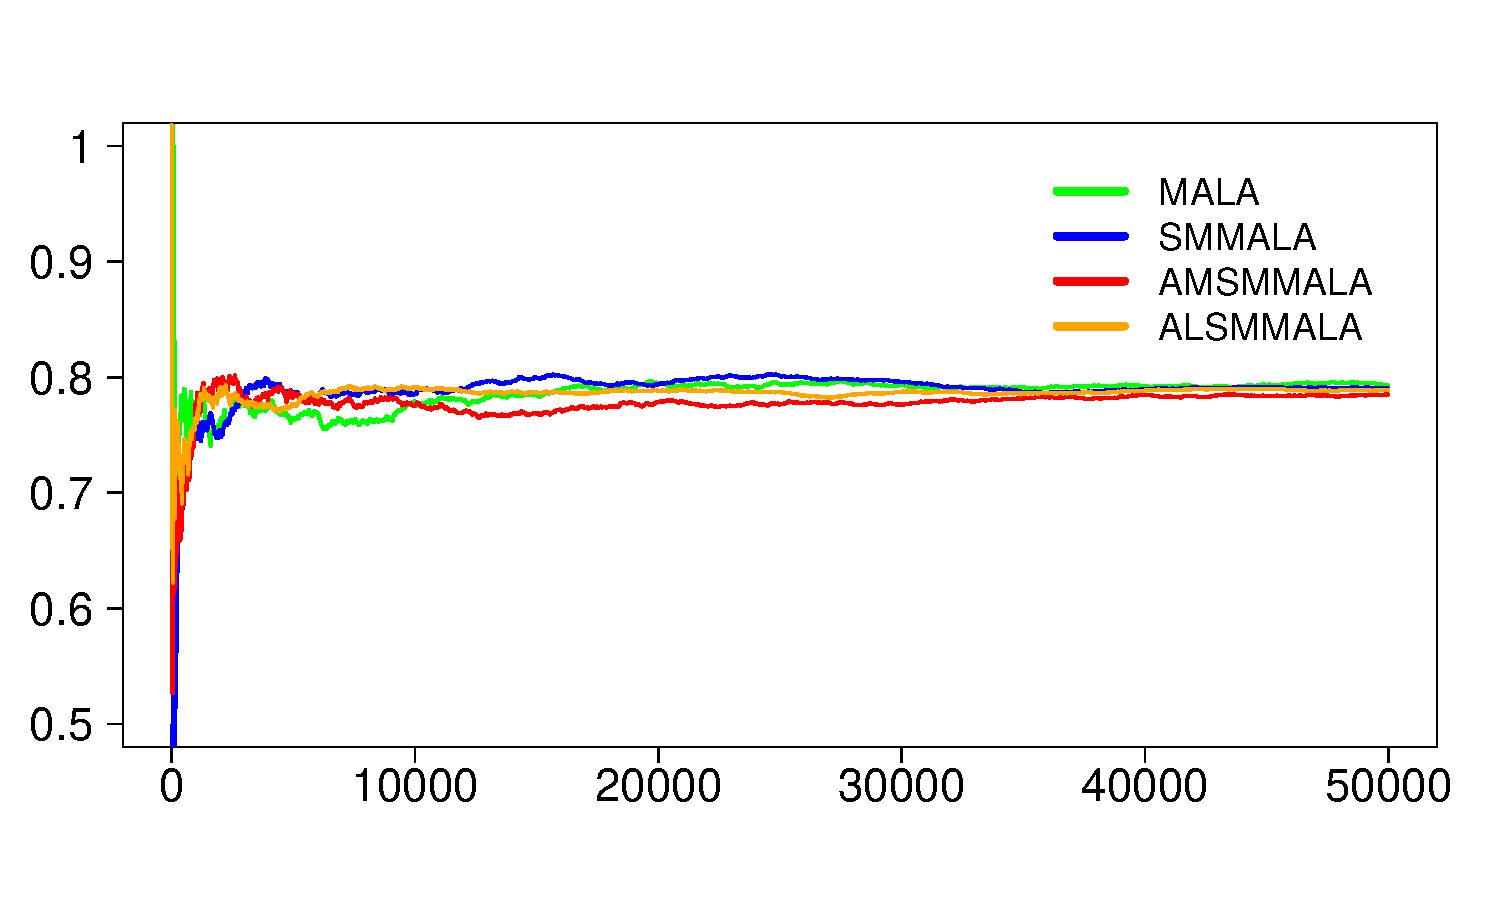
\includegraphics[width=2.8in]{logit_meanplot.pdf}
	} 
	\subfloat[Linear autocorrelation]{
	  \label{fig:logit:b}
		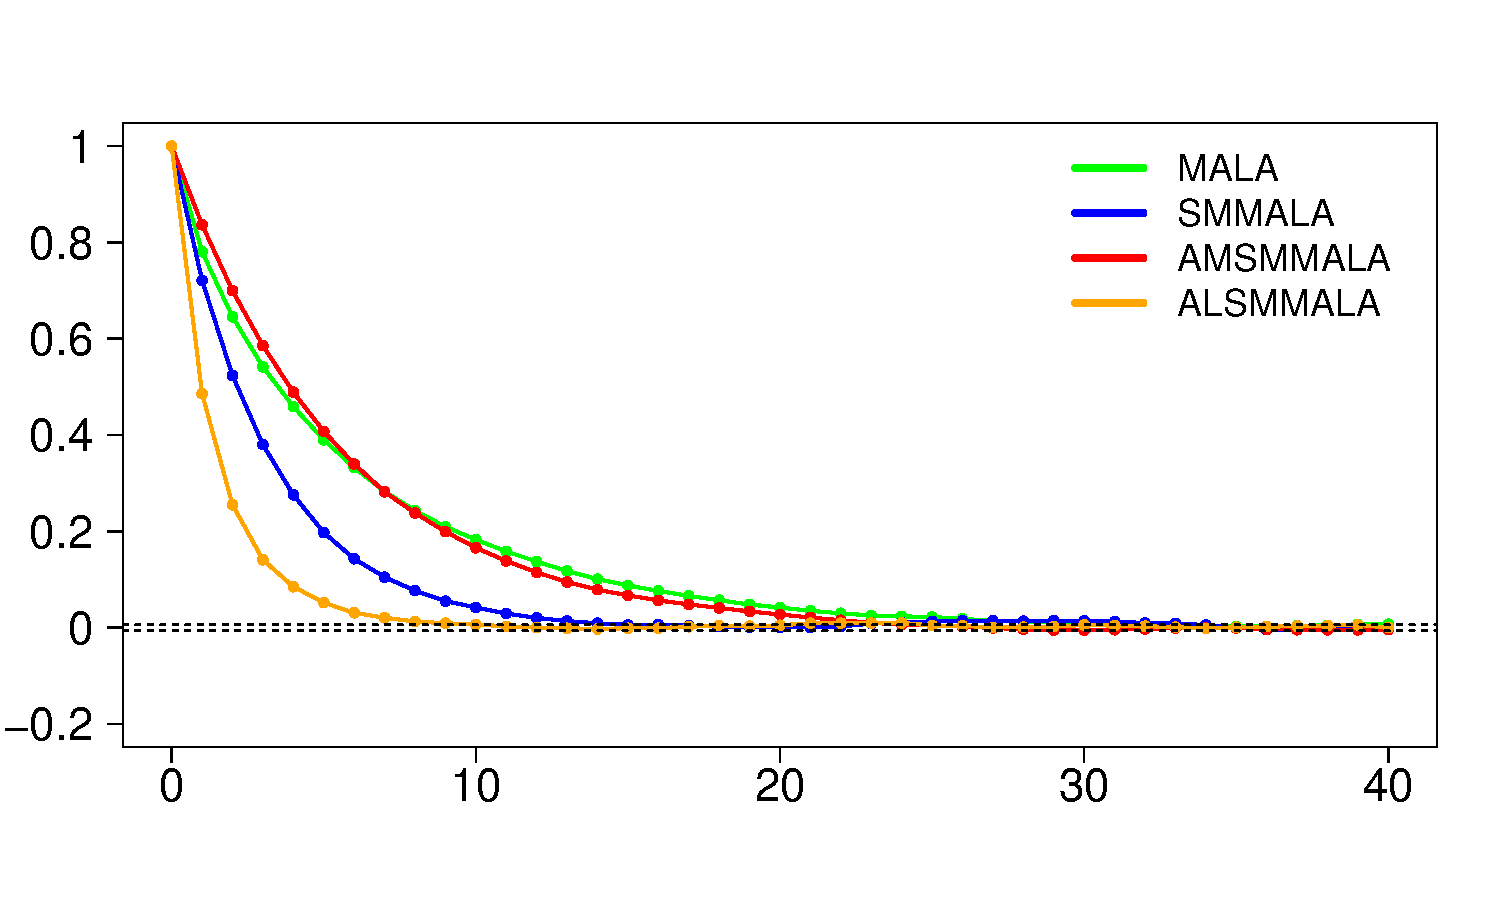
\includegraphics[width=2.8in]{logit_acfplot.pdf}
	} \\
	\subfloat[MALA traceplot]{
	  \label{fig:logit:c}		
		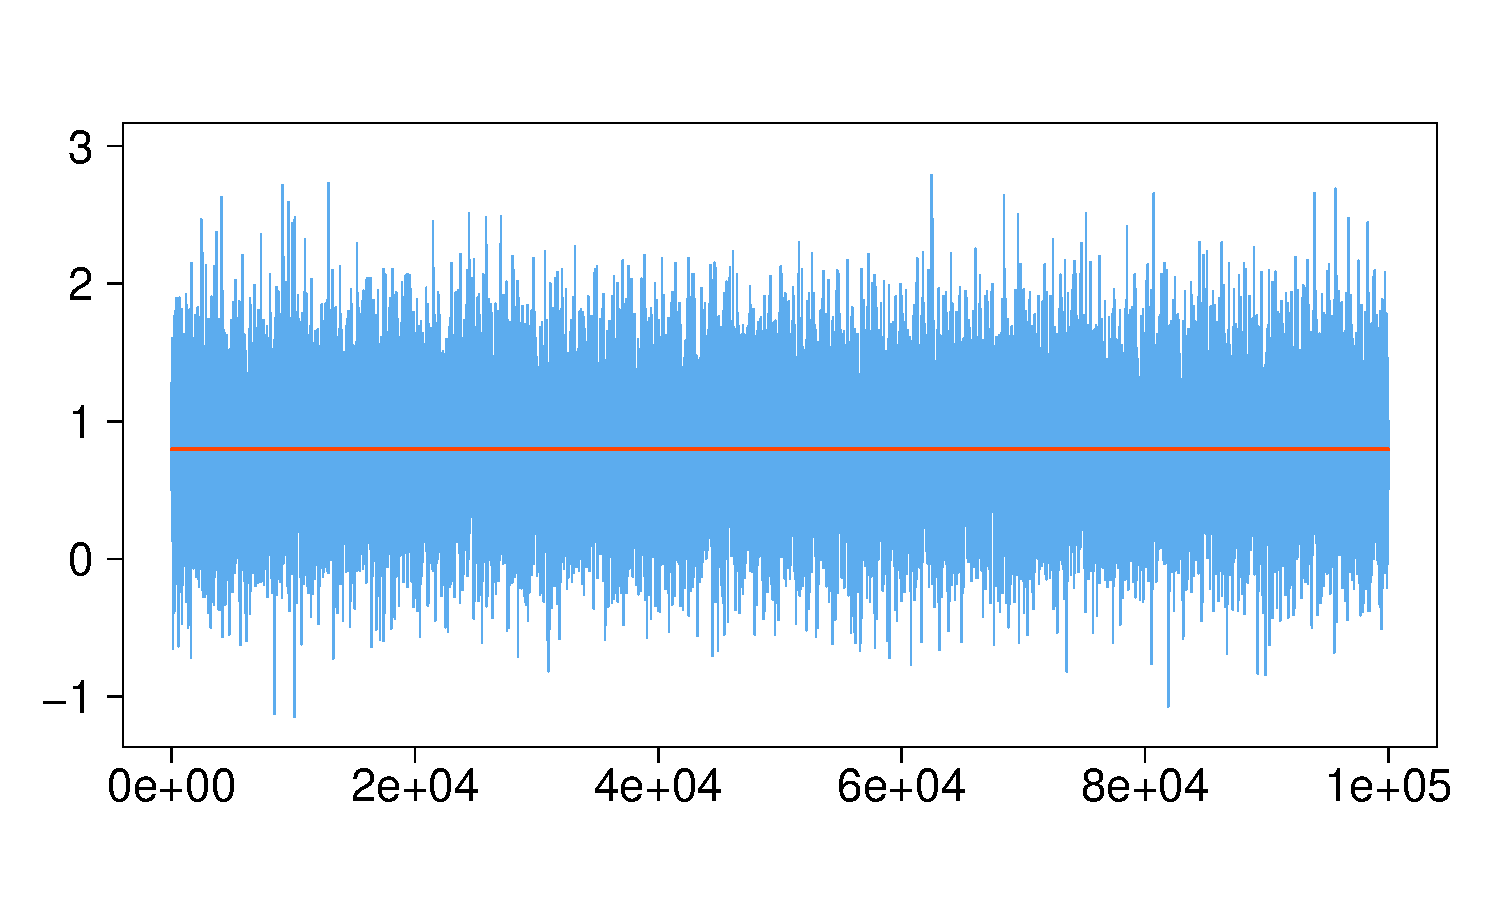
\includegraphics[width=2.8in]{logit_mala_traceplot.pdf}
	} 
	\subfloat[SMMALA traceplot]{
		\label{fig:logit:d}	
		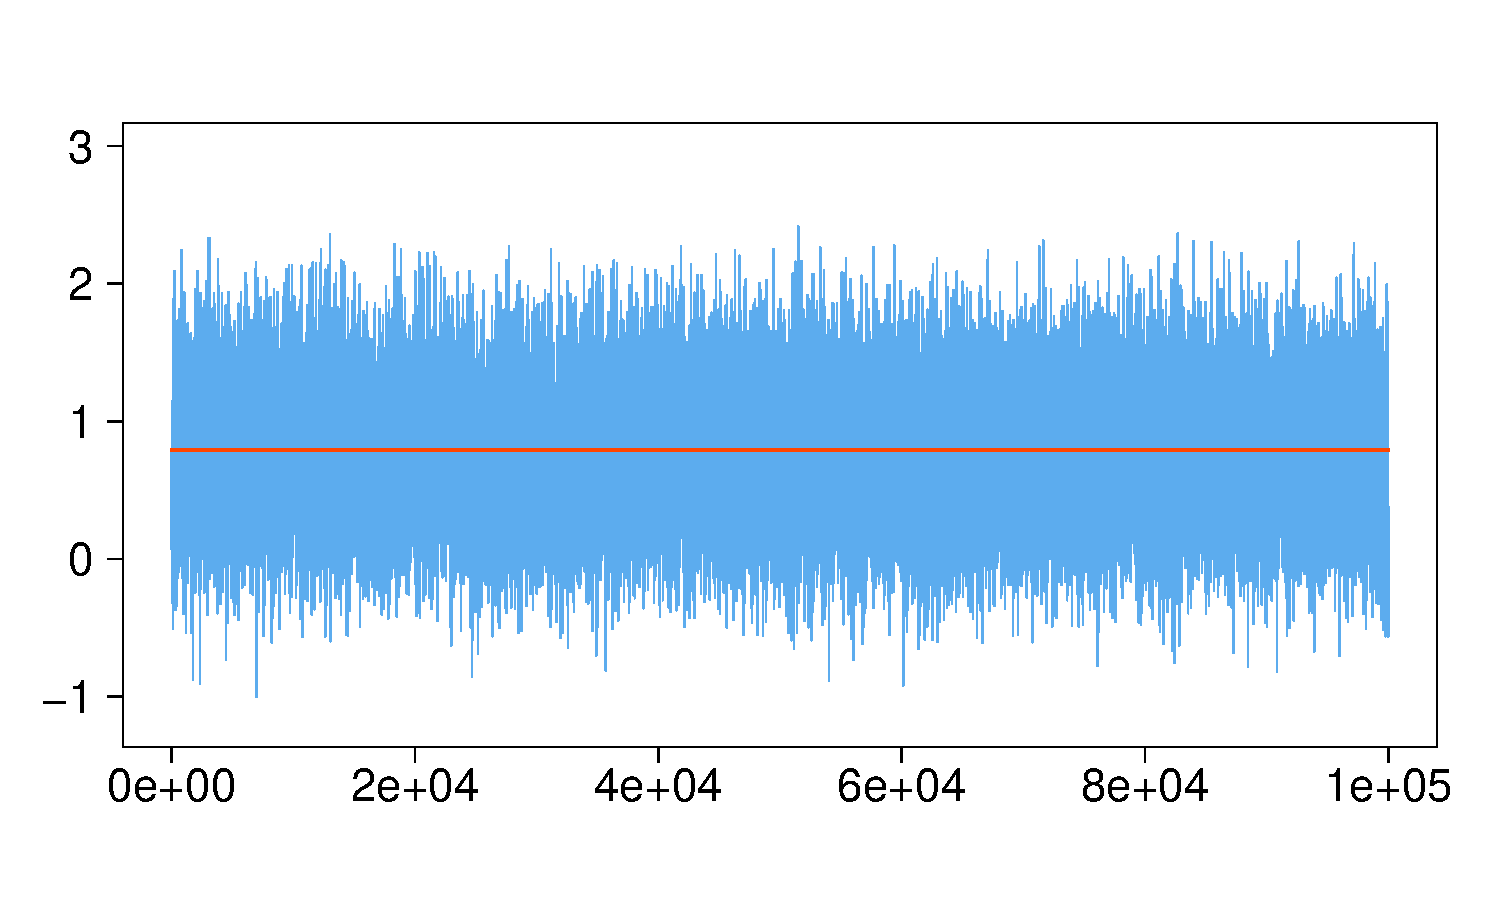
\includegraphics[width=2.8in]{logit_smmala_traceplot.pdf}
	} \\
	\subfloat[AMSMMALA traceplot]{
		\label{fig:logit:e}		
		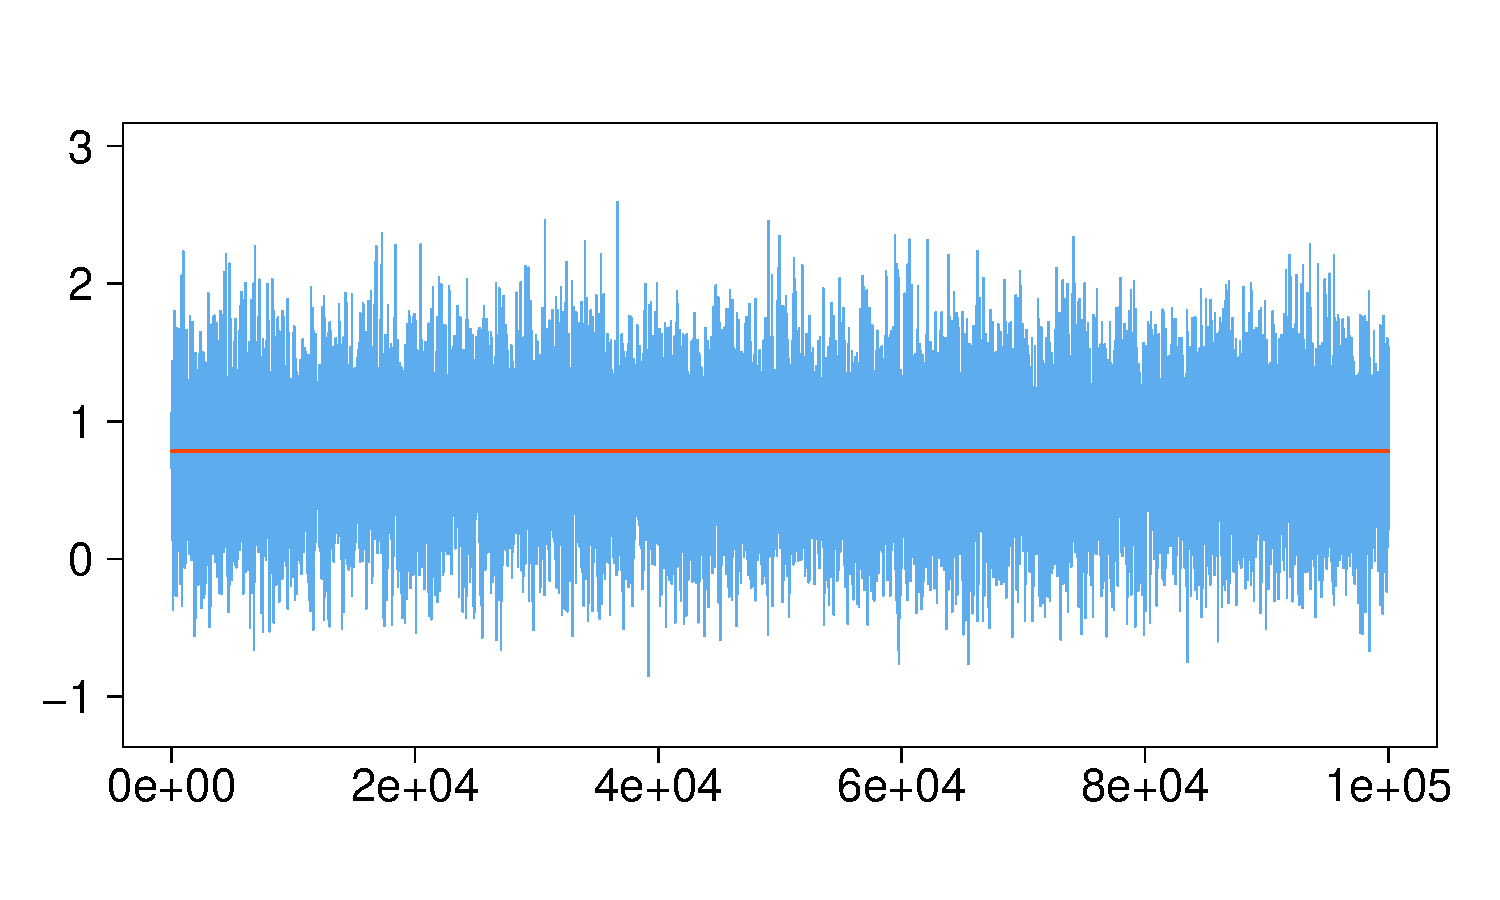
\includegraphics[width=2.8in]{logit_amsmmala_traceplot.pdf}
	}
	\subfloat[ALSMMALA traceplot]{
		\label{fig:logit:f}		
		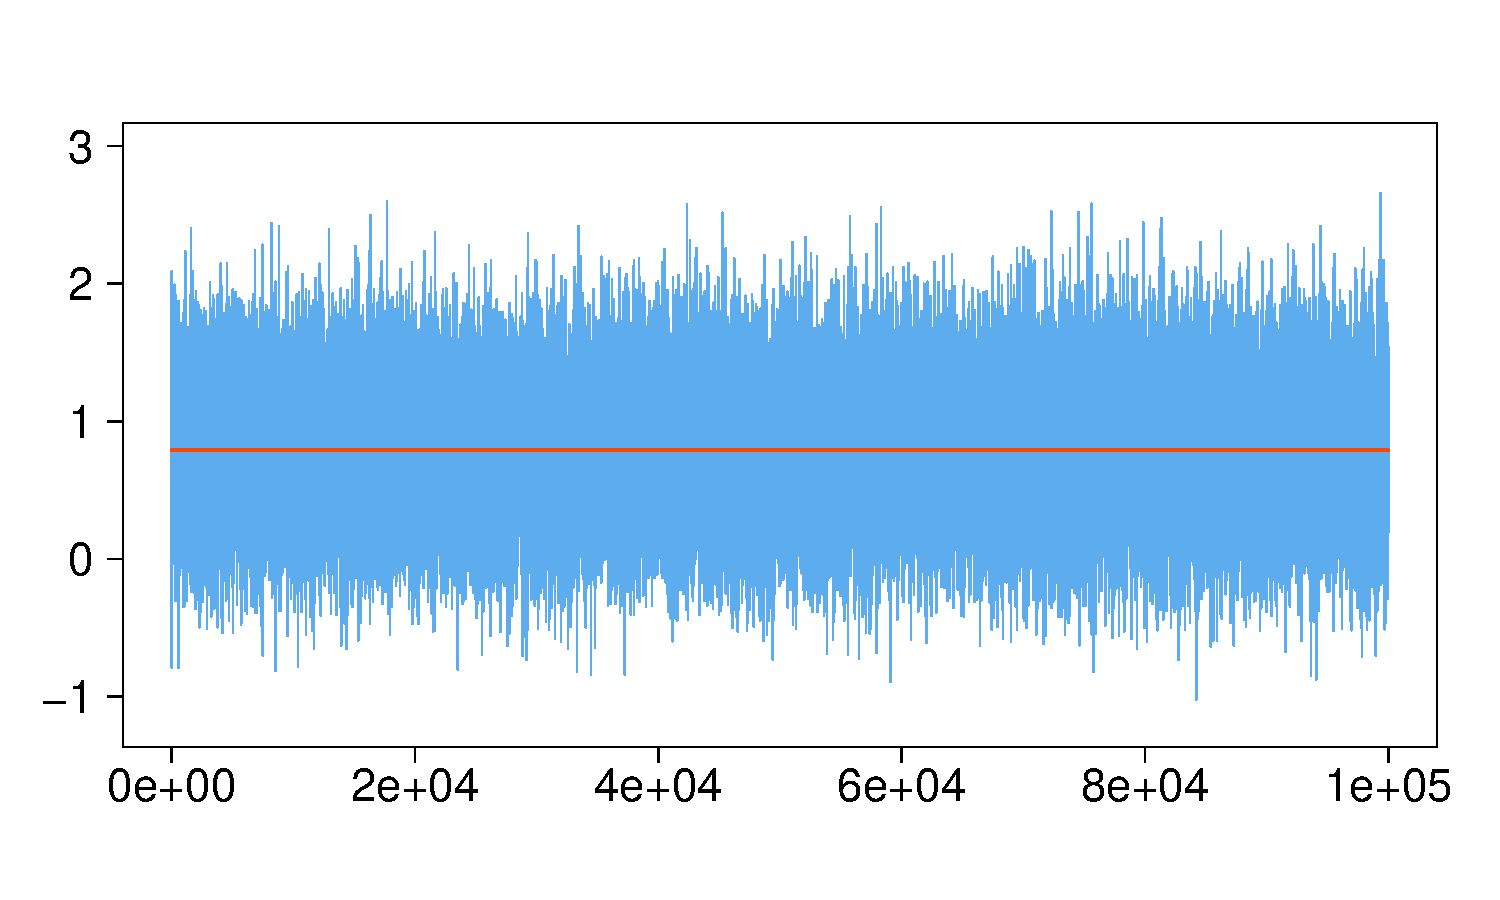
\includegraphics[width=2.8in]{logit_alsmmala_traceplot.pdf}
	} \\
	\caption{
		Plots of single chains corresponding to the regression coefficient of covariate $\boldsymbol{\theta}_{(2)}$ 
		simulated from each of MALA, SMMALA, AMSMMALA and ALSMMALA samplers by applying Bayesian logistic regression on the 
		Swiss banknotes data. (a) Overlaid running means, (b) overlaid linear autocorrelations for the four chains, (c)-(f) 
		individual traceplots per chain (the red horizontal lines represent the Monte Carlo mean).
	}
	\label{fig:logit}
\end{figure}

Figures \ref{fig:logit:c}-\ref{fig:logit:f} visualize the traceplots of four chains corresponding to the regression 
coefficient of covariate $\boldsymbol{\theta}_{(2)}$, with a single chain simulated from each of MALA, SMMALA, AMSMMALA and 
ALSMMALA using the Bayesian logistic regression log-target on the Swiss banknotes data. All four overlaid running means in 
Figure \ref{fig:logit:a}, plotted as a function of the number of iterations, demonstrate that the respective samplers 
converge towards the same value. The overlaid linear autocorrelations in Figure \ref{fig:logit:b} for the four chains 
exhibit magnitudes that agree with the effective sample sizes of Table \ref{tab:logit}. More specifically, ALSMMALA has the 
smallest linear autocorrelation and highest ESS by far, followed by SMMALA, while AMSMMALA and MALA have roughly the same 
linear autocorrelation and ESS. All four traceplots of MALA, SMMALA and of the two algorithms of this paper exhibit strong 
mixing properties.

\subsection{Bayesian Poisson Regression}

The log-likelihood of a Bayesian Poisson regression model with $n_d$ samples and $n_{\theta}$ covariates has the form
\begin{equation}
\label{eq:poisson_logl}
L(\mathbf{y}, X | \boldsymbol{\theta})=
(X\boldsymbol{\theta})^T\mathbf{y}-
\sum_{i=1}^{n_d}\left(
\exp(\boldsymbol{\theta}^T\mathbf{x_{i,}})
+\log{(y_i!)}
\right),
\end{equation}
where $\mathbf{y}\in\mathbb{R}^d$ is the response variable, $X$ the $n_d\cdot n_{\theta}$ design matrix and 
$\boldsymbol{\theta}\in\mathbb{R}^{n_{\theta}}$ the regression coefficients. By differentiating \eqref{eq:poisson_logl}, the 
gradient $\nabla_{\boldsymbol{\theta}}(L(\mathbf{y},X|\boldsymbol{\theta}))$ and the Hessian
$H(L(\mathbf{y}, X | \boldsymbol{\theta}))$ of the Bayesian Poisson log-likelihood are found to be
\begin{eqnarray}
\label{eq:poisson_gradlogl}
\nabla_{\boldsymbol{\theta}}(L(\mathbf{y},X|\boldsymbol{\theta}))=
X^T\left(\mathbf{y}-
\exp\left(X\boldsymbol{\theta}\right)\right),\\
\label{eq:plr:H}
H(L(\mathbf{y}, X | \boldsymbol{\theta}))=-X^T\mbox{diag}\left[\exp(\boldsymbol{\theta}^T\mathbf{x_{i,}})\right]X.
\end{eqnarray}

Assuming a normal prior $\boldsymbol{\theta}\sim\pi({\boldsymbol{\theta}})=\mathcal{N}(\boldsymbol{0},vI)$ with 
hyperparameter $v>0$, the unnormalized log-target of Bayesian Poisson regression is given by \eqref{eq:logit_target}
with the log-likelihood defined by \eqref{eq:poisson_logl}. Furthermore, the gradient of the log-target equals the sum of
\eqref{eq:poisson_gradlogl} and \eqref{eq:logit_gradlogprior}, while the associated metric
expresses as the negated sum $G(\boldsymbol{\theta}|X)=-H(L(\mathbf{y}, X | \boldsymbol{\theta}))+I/v$ of the log-likelihood 
Hessian \eqref{eq:plr:H} and of the log-prior Hessian $-I/v$.

MALA, SMMALA, ALSMMALA and AMSMMALA are run on a tropical tree data set using the Bayesian Poisson log-target of this 
section and the flat normal prior $\mathcal{N}(\boldsymbol{0},100I)$. The employed data are extracted from a big data set 
collected in the $500$ by $1000$ meter Barro Colorado Island plot in Panama (\cite{con_hub_fos__cha}). More specifically, 
the data used in this example describe the spatial positions in 1995 of $3605$ trees of the species Beilschmiedia pendula 
Lauraceae. Interest is in predicting the number of trees per unit area from the altitude and elevational gradient (slope) of 
the tree locations.

Before conducting MCMC inference, the altitude and gradient predictors are aggregated in a coarse $50$ by $50$ meter grid by
taking their means over the initial finer $5$ by $5$ meter grid. Figure \ref{fig:poisson_data} visualizes the tree locations 
and the coarsed data. Consequently, the processed data consist of the response variable $\mathbf{y}$ holding the number of 
trees in each of the $n_d=200$ coarse grid cells as well as the altitude and slop per coarse grid cell. The Poisson 
regression model comprises $n_{\theta}=4$ covariates, namely an intercept, the altitude and its square, and the elevational 
gradient.

\begin{figure}
	\centering
	\subfloat[Location of trees]{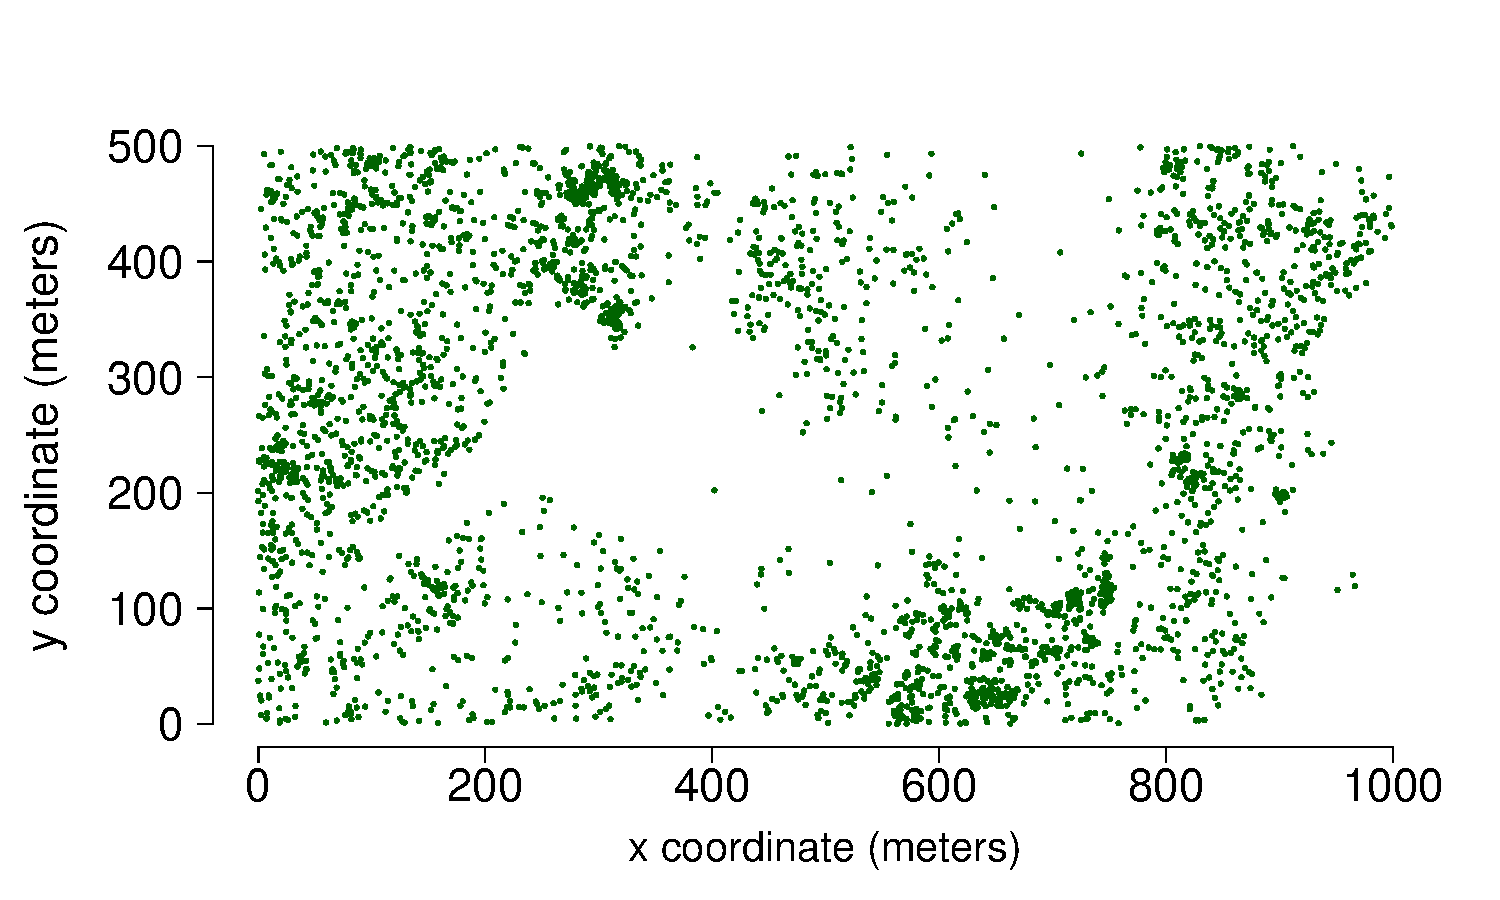
\includegraphics[width=2.8in]{tree_locations.pdf}} 
	\subfloat[Mean altitude per coarse grid cell]{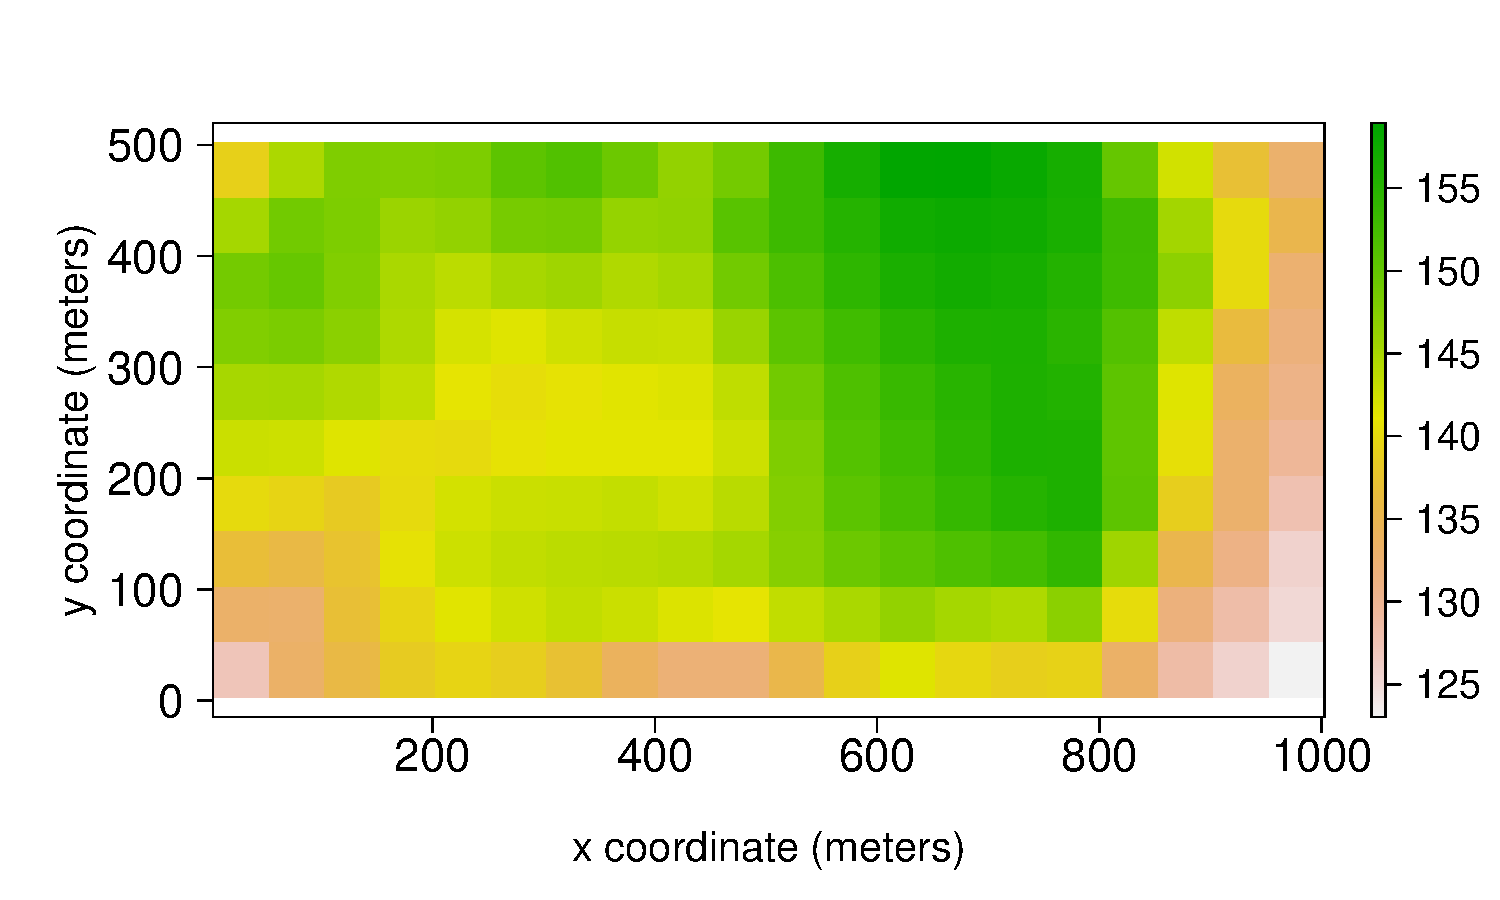
\includegraphics[width=2.8in]{tree_altitude.pdf}} \\
	\subfloat[Mean slope per coarse grid cell]{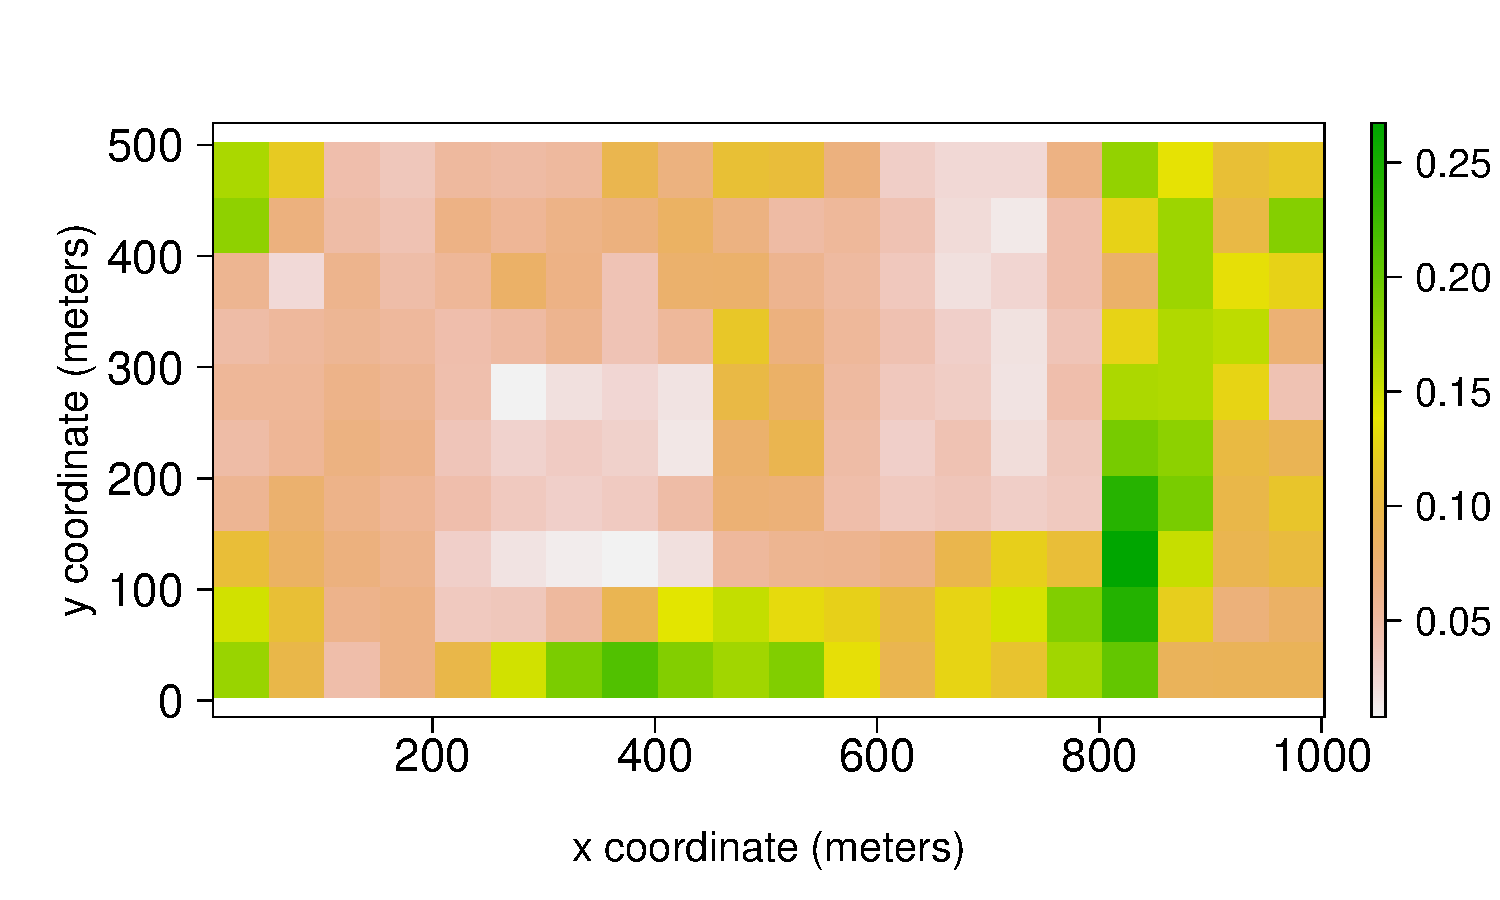
\includegraphics[width=2.8in]{tree_gradient.pdf}} 
	\subfloat[Number of trees per coarse grid cell]{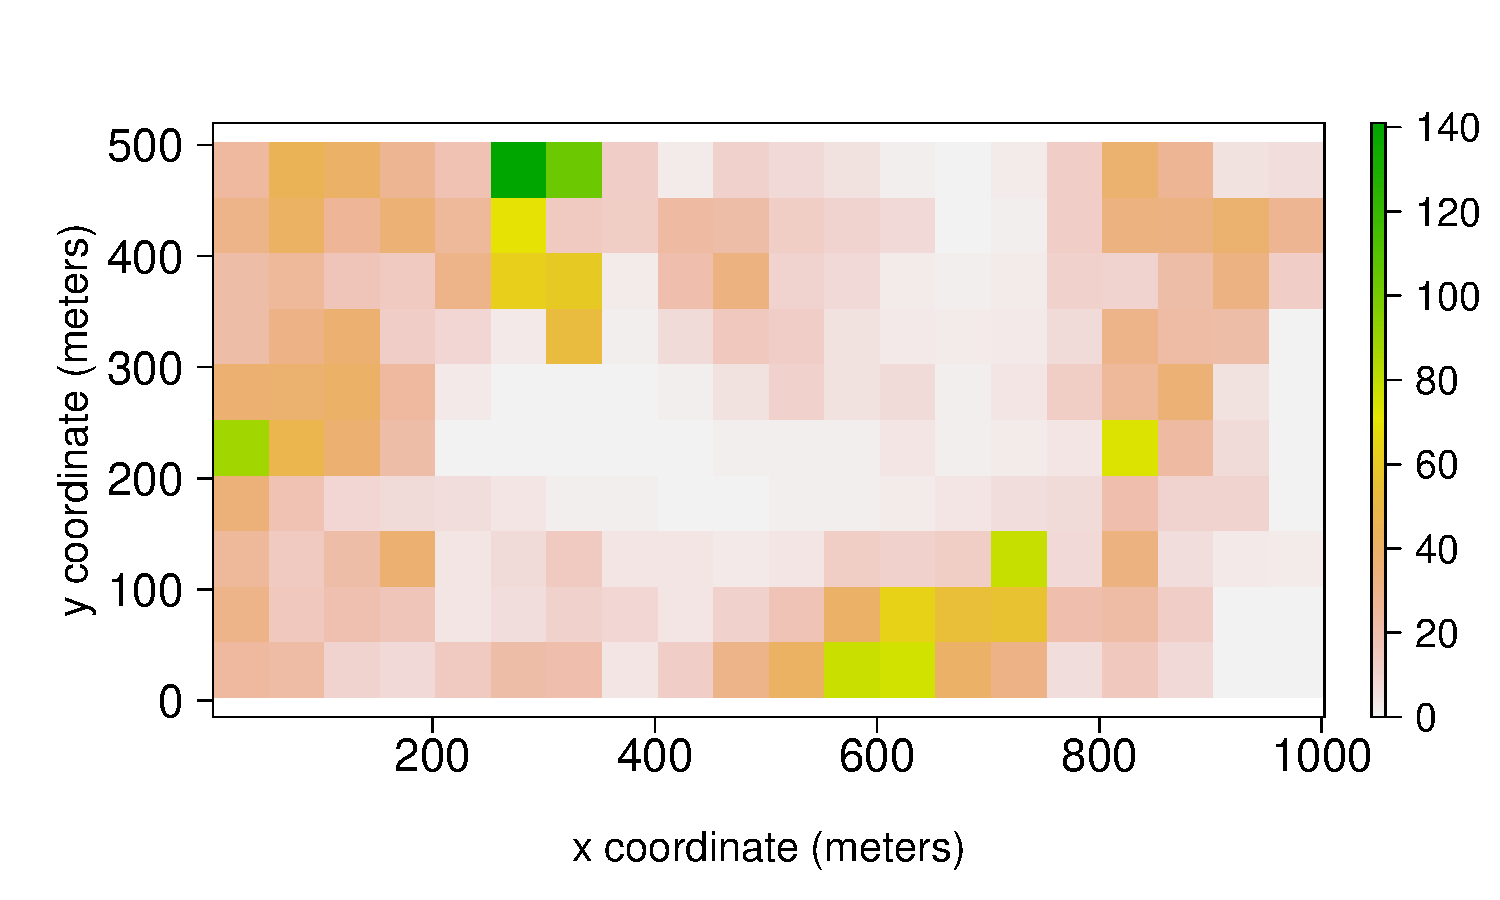
\includegraphics[width=2.8in]{tree_y.pdf}} \\
	\caption{Visualization of tree data of the species Beilschmiedia pendula Lauraceae collected in 1995 from the $500$ by 
	$1000$ meter Barro Colorado Island plot, Panama. (a): location of $3605$ observed trees (original data); (b)-(d): mean 
	altitude, mean elevational gradient and mean number of observed trees per coarse grid cell.}
	\label{fig:poisson_data}
\end{figure}

As it can be seen from the ESS of Table \ref{tab:poisson}, which is averaged across all ten simulated chains per sampler, 
and from the linear autocorrelation Figure \ref{fig:poisson:b}, which corresponds to a single simulated chain per sampler 
for the regression coefficient of altitude, two main groups of sampling effectiveness are formed. ALSMMALA and SMMALA 
acquire samples more effectively than AMSMMALA and MALA, plus it is observed that ALSMMALA having a marginal advantage over 
SMMALA. Moreover, ALSMMALA has smaller runtime than SMMALA. Overall, ALSMMALA stands out among all four samplers with a 
speedup of $2.09$ overtaking SMMALA. SMMALA exhibits a speedup of $1.03$, so it is doing better than MALA in this example. 
Although both ALSMMALA and SMMALA exploit local geometric information effectively, the former runs faster, hence it is 
preferred over latter. 

Figures \ref{fig:poisson:c}-\ref{fig:poisson:f} display the traceplots of four chains corresponding to the regression 
coefficient of covariate $\boldsymbol{\theta}_{(2)}$ (altitude), with a single chain simulated from each of MALA, SMMALA,
ALSMMALA and AMSMMALA. All four traceplots show that the involved samplers attain sufficient mixing. The overlaid running 
means of Figure \ref{fig:poisson:a} demonstrate that all four samplers converge to the same value for the coefficient 
corresponding to the altitude covariate.

\begin{table}
  \centering
	\begin{tabular}{l|r|rrrr|r|r|r}
		\hline\noalign{\smallskip}
		\multirow{2}{*}{Method} &
		\multirow{2}{*}{AR} &
		\multicolumn{4}{c|}{ESS} &
		\multirow{2}{*}{Time} &
		\multirow{2}{*}{Efficiency} &
		\multirow{2}{*}{Speedup} \\
		& & $\theta_1$ & $\theta_2$ & $\theta_3$ & $\theta_4$ & & & \\
		\noalign{\smallskip}\hline\noalign{\smallskip}
		MALA & .60 & 12649 & 14519 & 12942 & 32161 & 2.36 & 5354.88 & 1.00 \\
		SMMALA & .71 & 40132 & 39657 & 39522 & 39552 & 5.48 & 7212.76 & 1.35 \\
		AMSMMALA & .26 & 11812 & 11753 & 11675 & 11998 & 3.12 & 3740.16 & 0.70 \\
		ALSMMALA & .60 & 43157 & 43089 & 42892 & 43249 & 3.83 & 11194.52 & 2.09 \\
		\noalign{\smallskip}\hline
	\end{tabular}
	\caption{Comparison of sampling efficacy between MALA, SMMALA, AMSMMALA and ALSMMALA by applying Bayesian Poisson 
		regression on the tree data of the species Beilschmiedia pendula Lauraceae. AR: acceptance rate; ESS: effective sample 
		size; Time: CPU runtime in seconds; Efficiency: smaller ESS across four covariates divided by runtime; Speedup: ratio of 
		computational efficiencies with a MALA baseline. All the tabulated numbers have been rounded to the second decimal 
		place, apart from the effective sample sizes, which have been rounded to the nearest integer.}
	\label{tab:poisson}
\end{table}

\begin{figure}
	\centering
	\subfloat[Running mean]{
		\label{fig:poisson:a}
		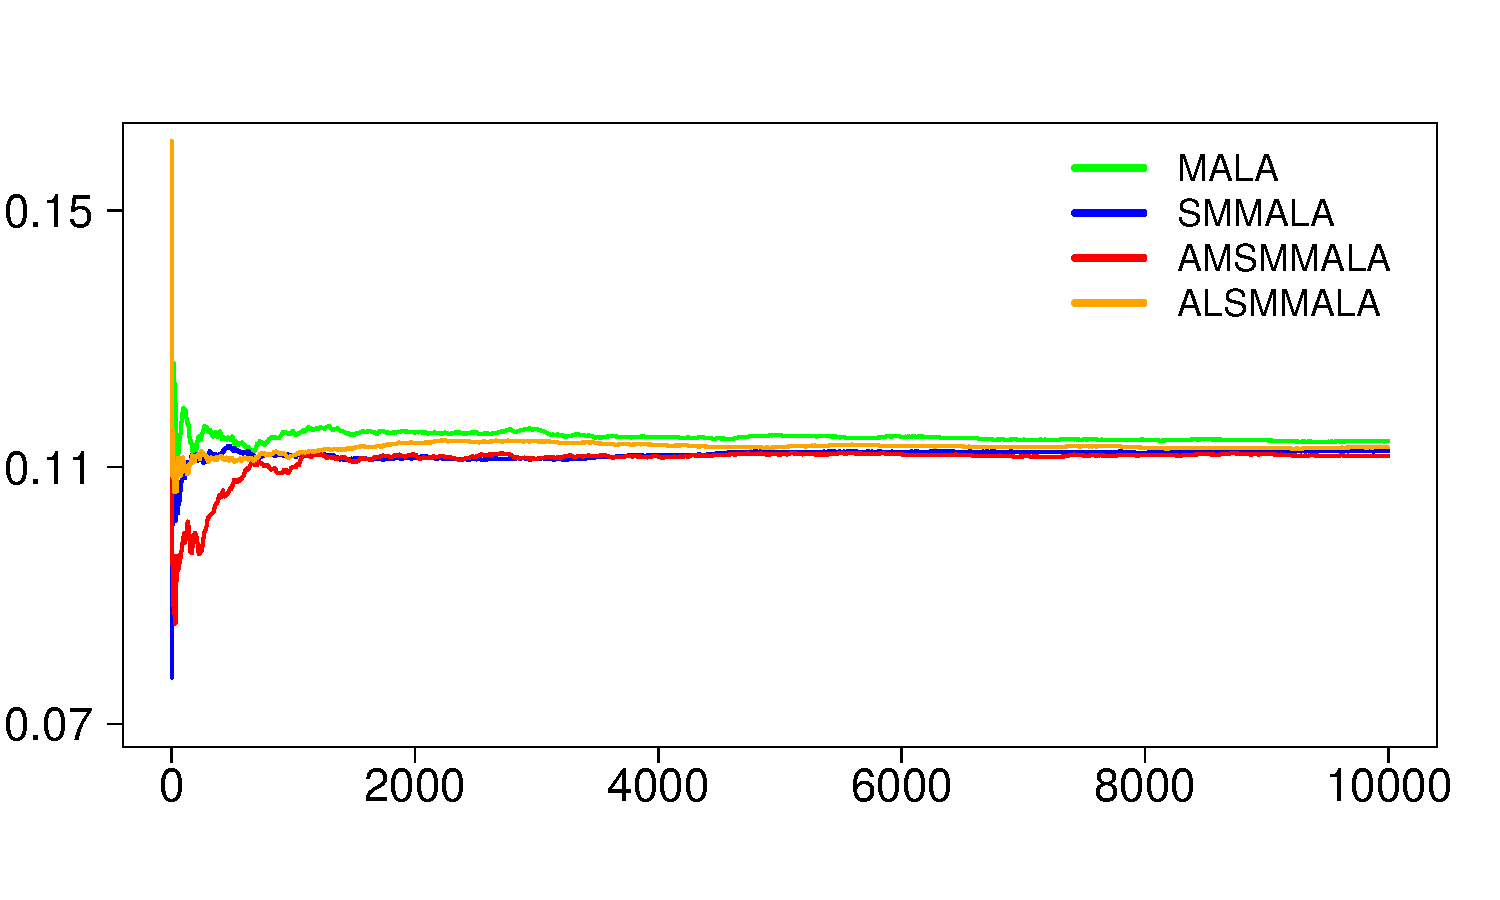
\includegraphics[width=2.8in]{poisson_meanplot.pdf}
	} 
	\subfloat[Linear autocorrelation]{
		\label{fig:poisson:b}
		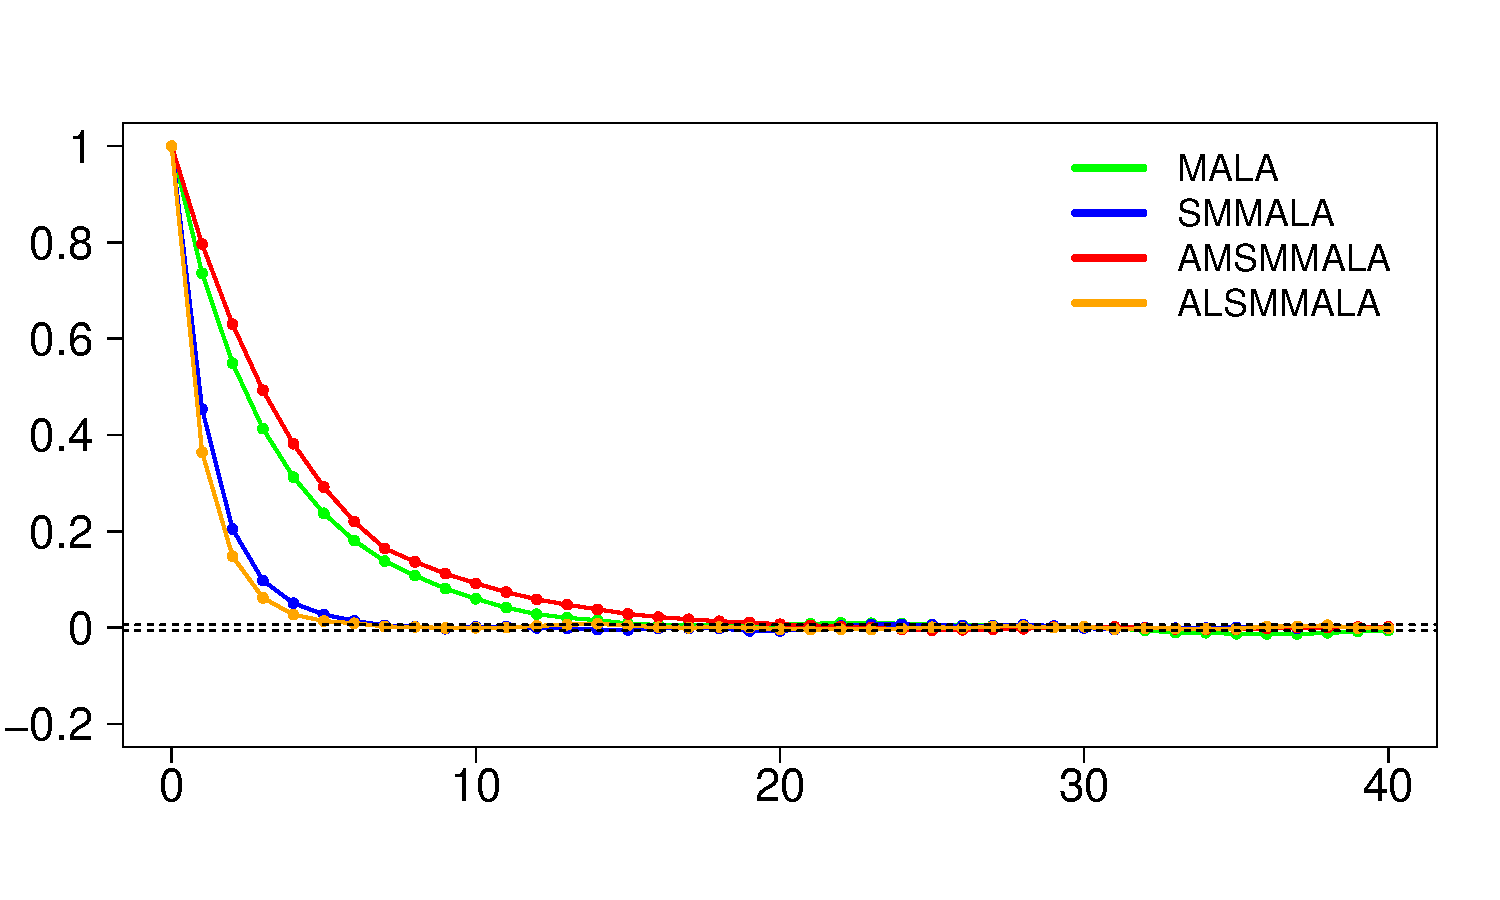
\includegraphics[width=2.8in]{poisson_acfplot.pdf}
	} \\
	\subfloat[MALA traceplot]{
		\label{fig:poisson:c}
		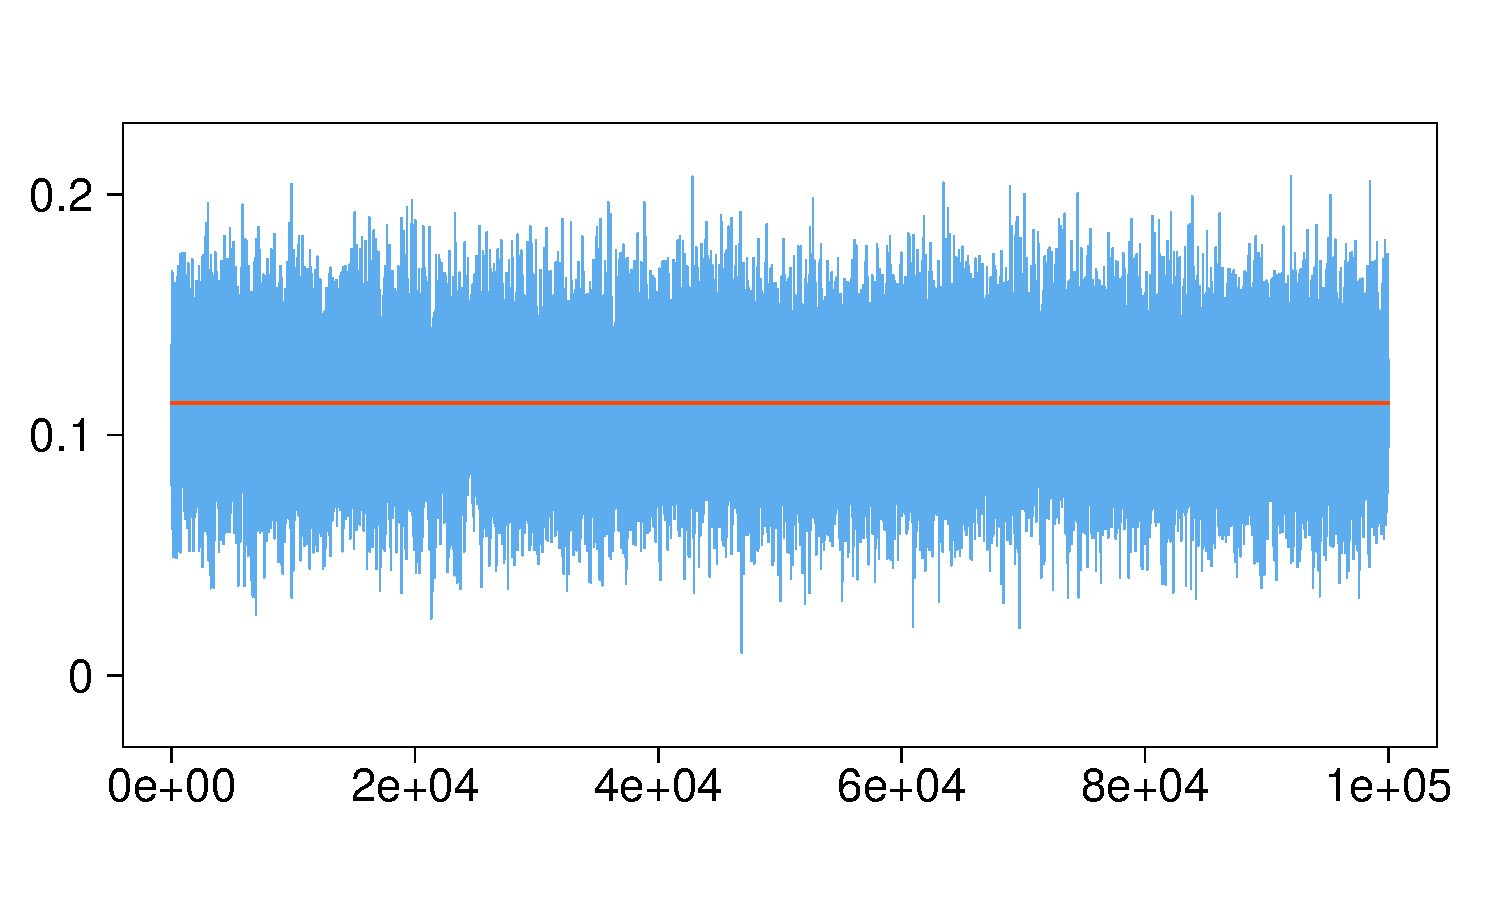
\includegraphics[width=2.8in]{poisson_mala_traceplot.pdf}
	} 
	\subfloat[SMMALA traceplot]{
		\label{fig:poisson:d}
		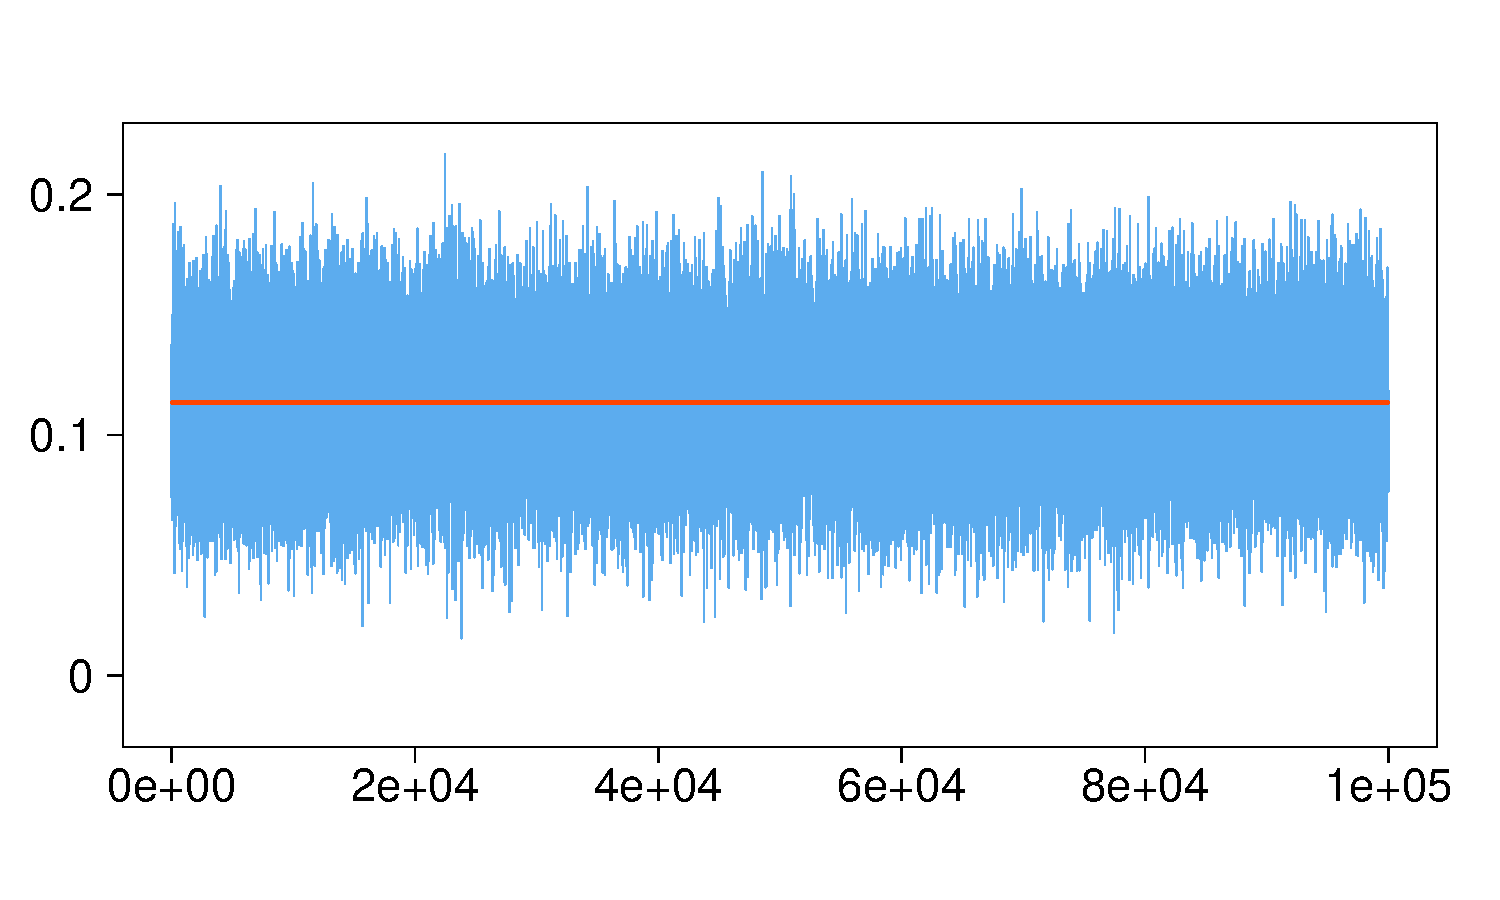
\includegraphics[width=2.8in]{poisson_smmala_traceplot.pdf}
	} \\
	\subfloat[AMSMMALA traceplot]{
		\label{fig:poisson:e}
		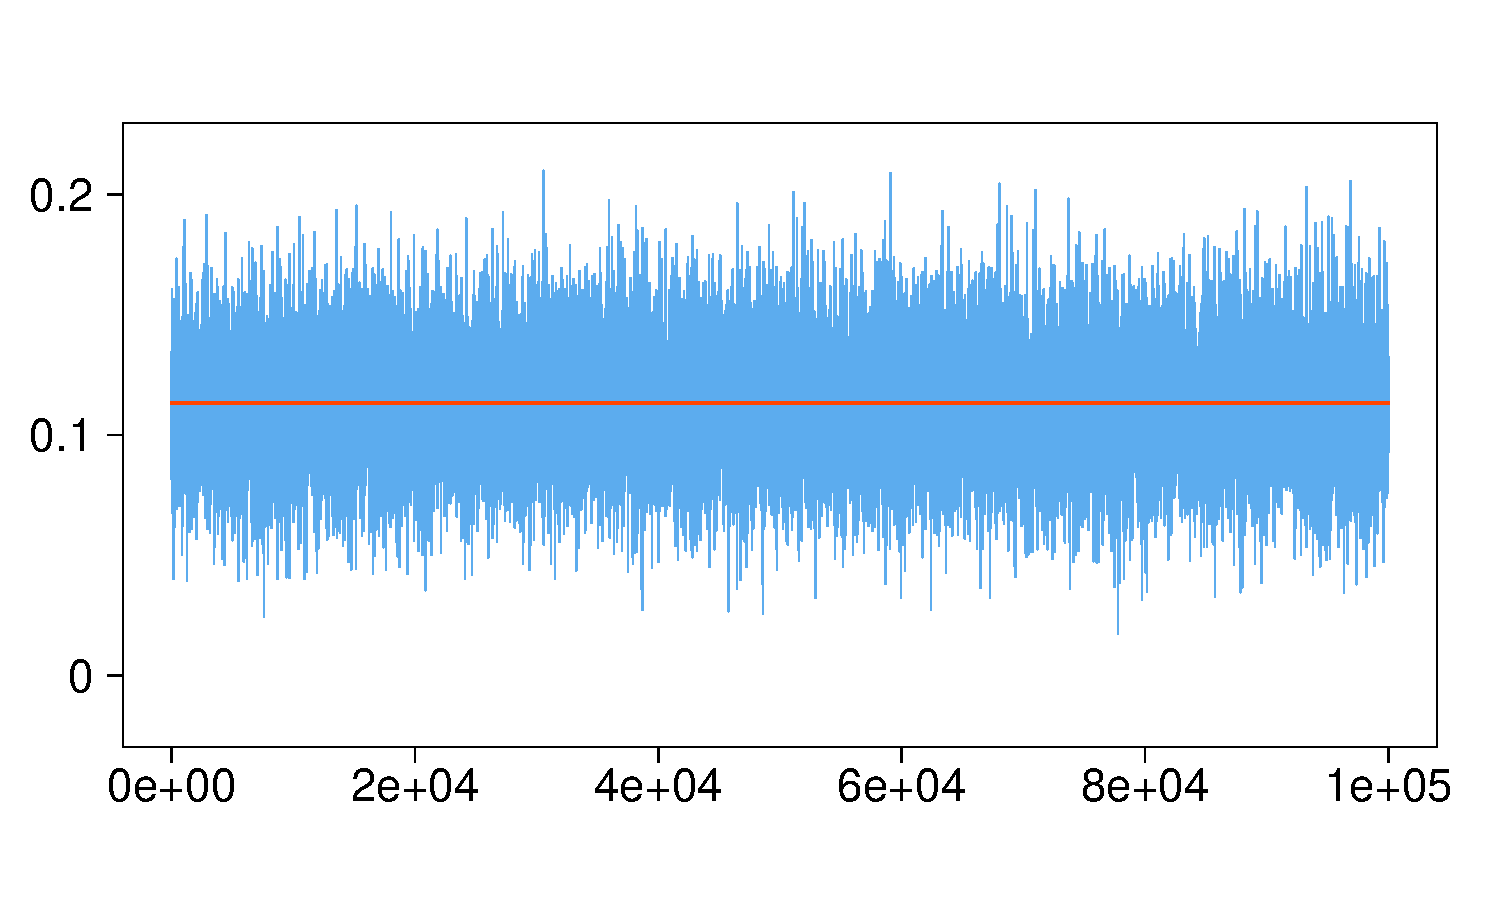
\includegraphics[width=2.8in]{poisson_amsmmala_traceplot.pdf}
	}
	\subfloat[ALSMMALA traceplot]{
		\label{fig:poisson:f}
		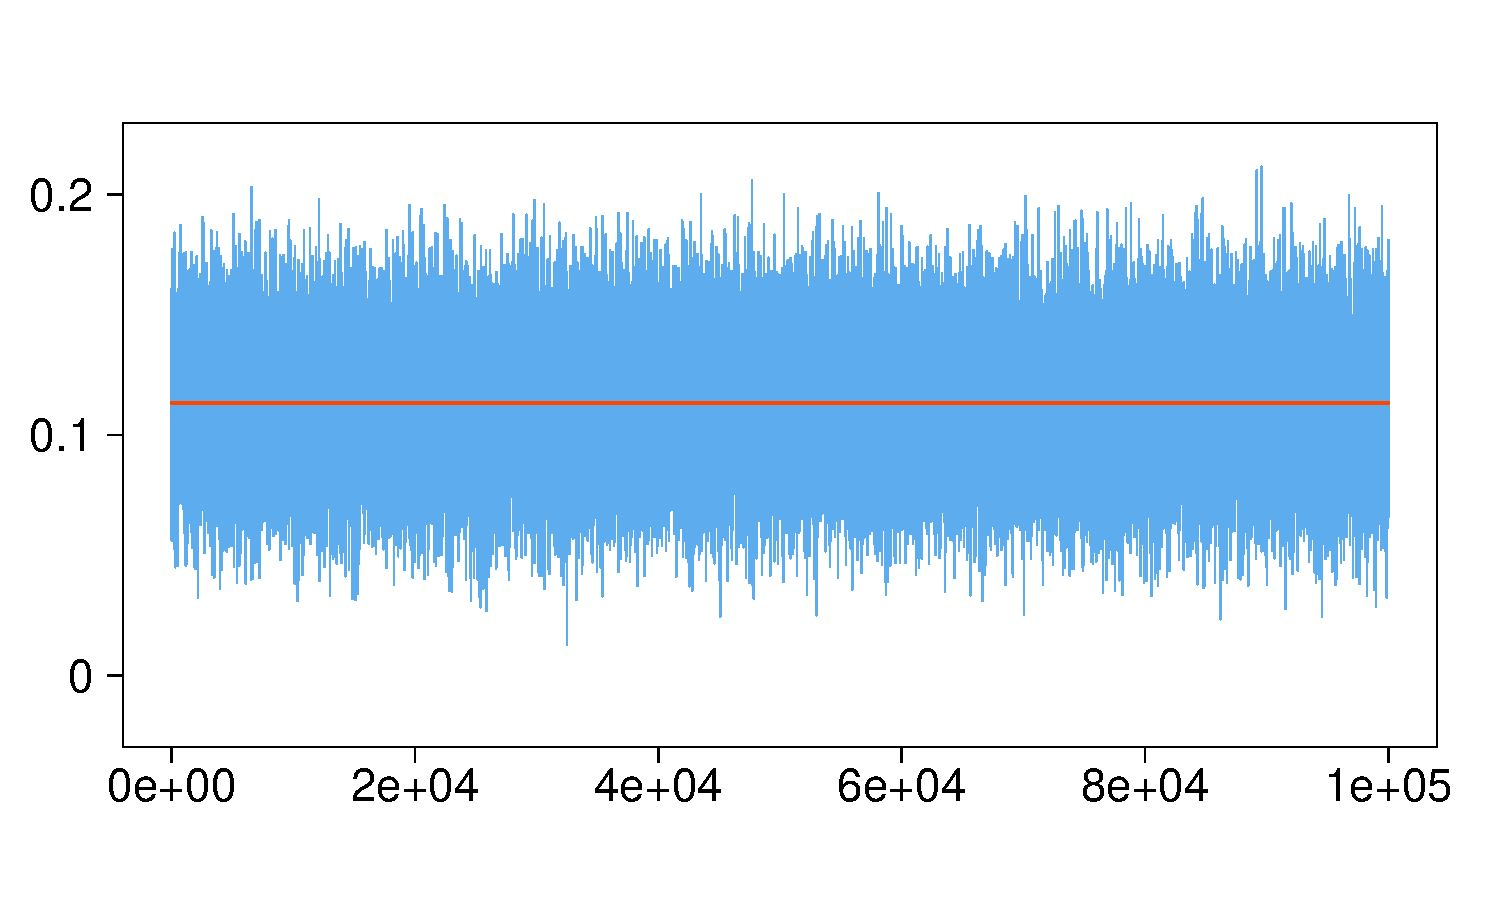
\includegraphics[width=2.8in]{poisson_alsmmala_traceplot.pdf}
	} \\ 
	\caption{Plots of single chains corresponding to the regression coefficient of the altitude covariate
		$\boldsymbol{\theta}_{(2)}$ simulated from each of MALA, SMMALA, AMSMMALA and ALSMMALA samplers by applying Bayesian 
		Poisson regression on the tree data of the species Beilschmiedia pendula Lauraceae. (a) Overlaid running means, (b) 
		overlaid linear autocorrelations for the four chains, (c)-(f) individual traceplots per chain (the red horizontal lines 
		represent the Monte Carlo mean).}
	\label{fig:poisson}
\end{figure}

\subsection{Multivariate $t$-Distribution}

Monte Carlo samples are drawn from an $n_{\theta}$-dimensional Student-$t$ target
$t_{\nu}(\mathbf{0},\frac{\nu-2}{\nu}\Sigma(c))$ with $\nu$ degrees of freedom and covariance matrix
\begin{equation}
\label{tp:eq:normal:sigma}
\Sigma(c)=\left(\begin{array}{ccccccc}
1 & c^1 & c^2 & \dots & c^{n_{\theta}-3} & c^{n_{\theta}-2} & c^{n_{\theta}-1} \\
c^1 & 1 & c^1 & \dots & c^{n_{\theta}-4} & c^{n_{\theta}-3} & c^{n_{\theta}-2} \\
c^2 & c^1 & 1 & \dots & c^{n_{\theta}-5} & c^{n_{\theta}-4} & c^{n_{\theta}-3} \\
\vdots & \vdots & \vdots & \ddots & \vdots & \vdots & \vdots \\
c^{n_{\theta}-3} & c^{n_{\theta}-4} & c^{n_{\theta}-5} & \dots & 1 & c^{1} & c^{2} \\
c^{n_{\theta}-2} & c^{n_{\theta}-3} & c^{n_{\theta}-4} & \dots & c^{1} & 1 & c^{1} \\
c^{n_{\theta}-1} & c^{n_{\theta}-2} & c^{n_{\theta}-3} & \dots & c^{2} & c^1 & 1 \\
\end{array}\right),
\end{equation}
for some constant $0<c<1$ that determines the level of correlation between parameter dimensions. The elements of the 
$i$-th diagonal of the $n_{\theta}\times n_{\theta}$ covariance matrix $\Sigma(c)$ equal $c^{i-1},~i=1,2,\dots,n_{\theta}$.
The scale matrix $\frac{\nu-2}{\nu}\Sigma(c)$ of the $t$-distribution scales $\Sigma(c)$ by a factor of $(\nu-2)/\nu$ so that 
the covariance matrix of the $t$-distribution is $\Sigma(c)$.

% NOTE:  Couldn't we make this Bayesian by placing a uniform prior on the mean?
In this example, the setting is not Bayesian, so there is no prior distribution involved. Instead, MCMC is used for drawing
samples from a Student-$t$ distribution $t_{\nu}(\mathbf{0},\frac{\nu-2}{\nu}\Sigma(c))$ acting as a random number generator. 
The simulated chains are randomly initialized away from the zero mode of the $t$-distribution, and they are expected to 
converge to zero. In other words, the zero mode of $t_{\nu}(\mathbf{0},\frac{\nu-2}{\nu}\Sigma(c))$ is seen as the parameter 
vector to be estimated.

To emulate some of the conditions of real-life applications, the dimension of the $t$-target in the MCMC simulations is 
increased to $n_{\theta}=20$ from the $n_{\theta}=4$ dimensions of Bayesian logistic and Poisson regression models, 
relatively high correlation is induced by selecting $c=0.9$ in \eqref{tp:eq:normal:sigma}, and some amount of probability 
mass is maintained in the distribution tails by choosing $\nu=30$ degrees of freedom. Furthermore, automatic differentiation 
is employed instead of deriving the gradient and Hessian of the $t$-target analytically and the SoftAbs metric is used for 
correcting the indefinite inverse metric evaluations arising in the course of simulations. Of course the present example does
not reach the realm of a fully-fledged application, especially in terms of log-target complexity, but it gives a first
indication of other common computational costs appearing in more realistic applications.

Table \ref{tab:t} reports the minimum, median and maximum ESS of the $n_{\theta}=20$ parameter dimensions after averaging 
across the ten simulated chains per sampler. As seen from Table \ref{tab:t}, MALA and SMMALA struggle with the 
$t$-distribution yielding very low effective sample size. This is explained by the fact that Langevin Monte Carlo does not 
produce geometrically ergodic chains for targets with heavier tails. ALSMMALA also does poorly in terms of ESS, albeit 
somewhat better than its Langevin proposal counterparts. ALSMMALA is impractical for this example, because it reaches its 
optimal ESS for the simulated $t$-target after empirical tuning that results in a high acceptance rate of $0.96$. Besides, 
ALSMMALA is somewhat unstable in the sense that if the acceptance rate is not very close to $0.95$ then ESS drops 
dramatically. After all, ALSMMALA is in essence a Langevin Monte Carlo sampler, so it is not anticipated to overcome the 
intrinsic limitations of its MALA and SMMALA proposal kernels.

On the other hand, AMSMMALA attains much higher ESS than the three Langevin-centric samplers. The AM algorithm of 
\cite{haa_sak_tam__ana} is not directly applicable to a $t$-target for two reasons. The original AM sampler is designed to 
work with targets of bounded support; this shortcoming can be circumvented by a truncated proposal. However, the AM sampler 
assumes that the probability mass of the target vanishes outside the region of support, so the $t$-target can not be 
accommodated directly by the AM algorithm as initially conceived by \cite{haa_sak_tam__ana}. Empirical validation via 
simulations shows that AMSMMALA converges to the mode of the simulated $t$-target despite the heavier target tails and 
correlation between parameter dimensions. In other words, AMSMMALA offers a new algorithm with greater range of applicability
than its AM proposal kernel. This is explained by the recurring local geometric corrections of the empirical covariance via 
SMMALA steps. It is worth noticing that Metropolis-Hastings is less effective than Langevin Monte Carlo samplers, such as 
MALA and SMMALA, in the case of the simulated $t$-target, so AMSMMALA offers a viable way to simulate from the Student 
$t$-distribution of this example, where its contestants fail. In the future, it would be of interest to further compare 
AMSMMALA with other adaptive Metropolis samplers such as the random adaptive Metropolis (RAM) sampler by \cite{vih__rob} and 
the adaptive Metropolis-within-Gibbs (AMWG) algorithm by \cite{rob_ros__exa}.

SMMALA has been run using two modes of automatic differentiation, namely reverse AD with source transformation and forward 
mode. The average SMMALA runtime across ten simulations with forward mode is $575.29$ seconds, roughly fourteen times slower
than the respective runtime of $41.39$ seconds for SMMALA with reverse mode. In spite of using the ForwardDiff Julia 
package (\cite{rev_lub_pap__for}), which benefits from tuples that are stack-allocated instead of being heap-allocated, the
computational cost for forward mode AD remains prohibitive for this example and for probabilistic problems more generally.

AMSMMALA has an average runtime of $15.13$ seconds, and therefore attains a threefold increase in execution time in
comparison to SMMALA when both samplers rely on reverse mode. Overall, AMSMMALA achieves a speedup factor of $7.75$ thanks to
its increased ESS and speed of execution.

Figure \ref{fig:t} visualizes the output of four chains that correspond to the seventh dimension $\boldsymbol{\theta}_{(7)}$
of the $20$-dimensional $t$-target $t_{30}(\mathbf{0},\frac{28}{30}\Sigma(0.9))$, with a single chain simulated from each of 
MALA, SMMALA, ALSMMALA and AMSMMALA. Figure \ref{fig:t:b} shows the substantial reduction in linear autocorrelation achieved 
by AMSMMALA, leading to optimal ESS among the four compared samplers. ALSMMALA also reduces the linear autocorrelation, 
although it is not the sampler of choice for the $t$-target. As seen from Figure \ref{fig:t:a}, the running means of AMSMMALA 
and ALSMMALA converge to the same value, as opposed to the means of MALA and SMMALA. The traceplots of Figures 
\ref{fig:t:c}-\ref{fig:t:f} demonstrate the superior mixing of AMSMMALA and the problematic mixing of MALA and SMMALA for 
the $t$-target of this example.

\begin{table}
	\begin{tabular}{l|r|rrr|r|r|r}
		\hline\noalign{\smallskip}
		\multirow{2}{*}{Method} &
		\multirow{2}{*}{AR} &
		\multicolumn{3}{c|}{ESS} &
		\multirow{2}{*}{Time} &
		\multirow{2}{*}{Efficiency} &
		\multirow{2}{*}{Speedup} \\
		& & mean & median & max & & & \\
		\noalign{\smallskip}\hline\noalign{\smallskip}
		MALA & .60 & 127 & 145 & 239 & 1.95 & 65.09 & 1.00 \\
		SMMALA (r) & .67 & 103 & 114 & 123 & 41.39 & 2.48 & 0.04 \\
		SMMALA (f) & .68 & 97 & 104 & 121 & 575.29 & 0.17 & 0.00 \\
		AMSMMALA & .16 & 7629 & 7863 & 7922 & 15.13 & 504.11 & 7.75 \\
		ALSMMALA & .96 & 2465 & 2538 & 2574 & 16.16 & 152.51 & 2.34 \\	
		\noalign{\smallskip}\hline
	\end{tabular}
	\caption{Comparison of sampling efficacy between MALA, SMMALA, AMSMMALA and ALSMMALA by sampling from the $20$-dimensional
		$t$-target $t_{30}(\mathbf{0},\frac{28}{30}\Sigma(0.9))$. AR: acceptance rate; ESS: effective sample size; Time: CPU 
		runtime in seconds; Efficiency: smaller ESS across four covariates divided by runtime; Speedup: ratio of computational 
		efficiencies with a MALA baseline. All the tabulated numbers have been rounded to the second decimal place, apart from 
		the effective sample sizes, which have been rounded to the nearest integer.}
	\label{tab:t}
\end{table}

\begin{figure}
	\centering
	\subfloat[Running mean]{
	  \label{fig:t:a}
		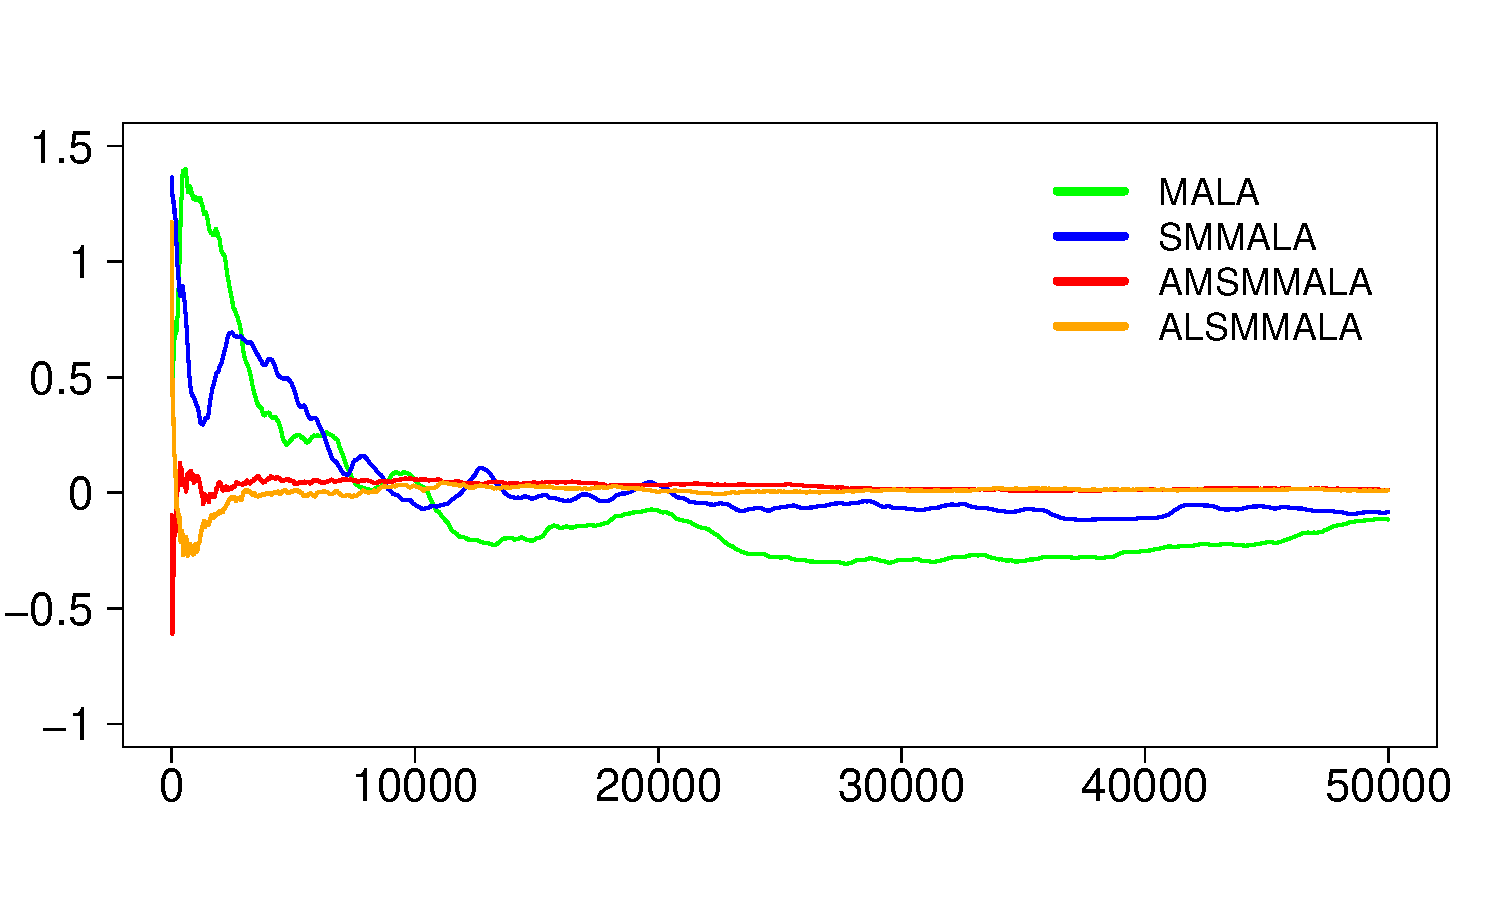
\includegraphics[width=2.8in]{tdist_meanplot.pdf}
	} 
	\subfloat[Linear ACF]{
  	\label{fig:t:b}
		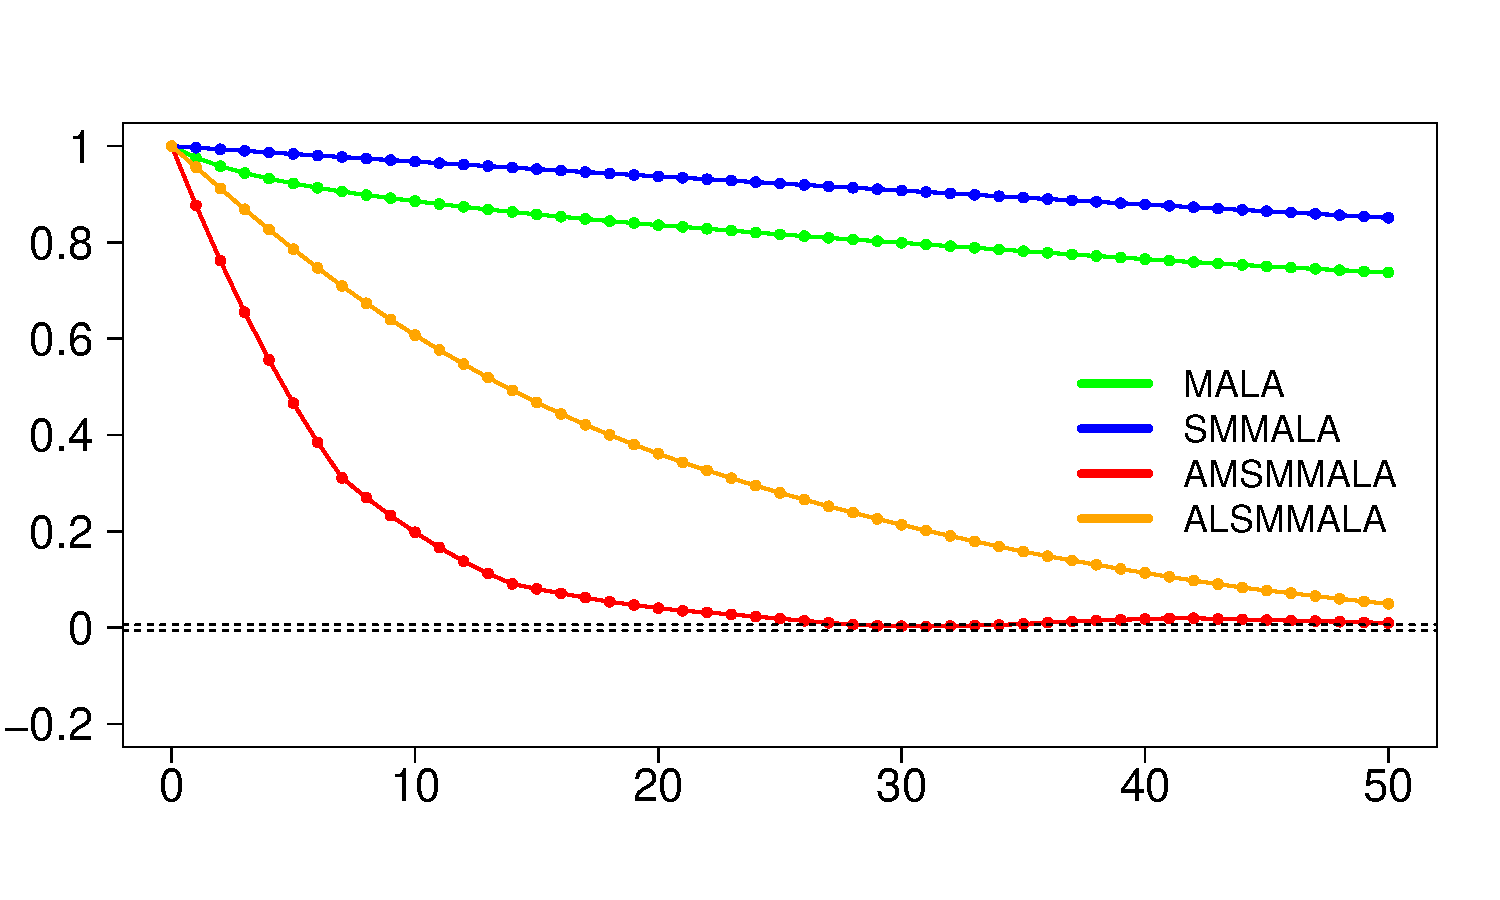
\includegraphics[width=2.8in]{tdist_acfplot.pdf}
	} \\
	\subfloat[MALA traceplot]{
		\label{fig:t:c}
		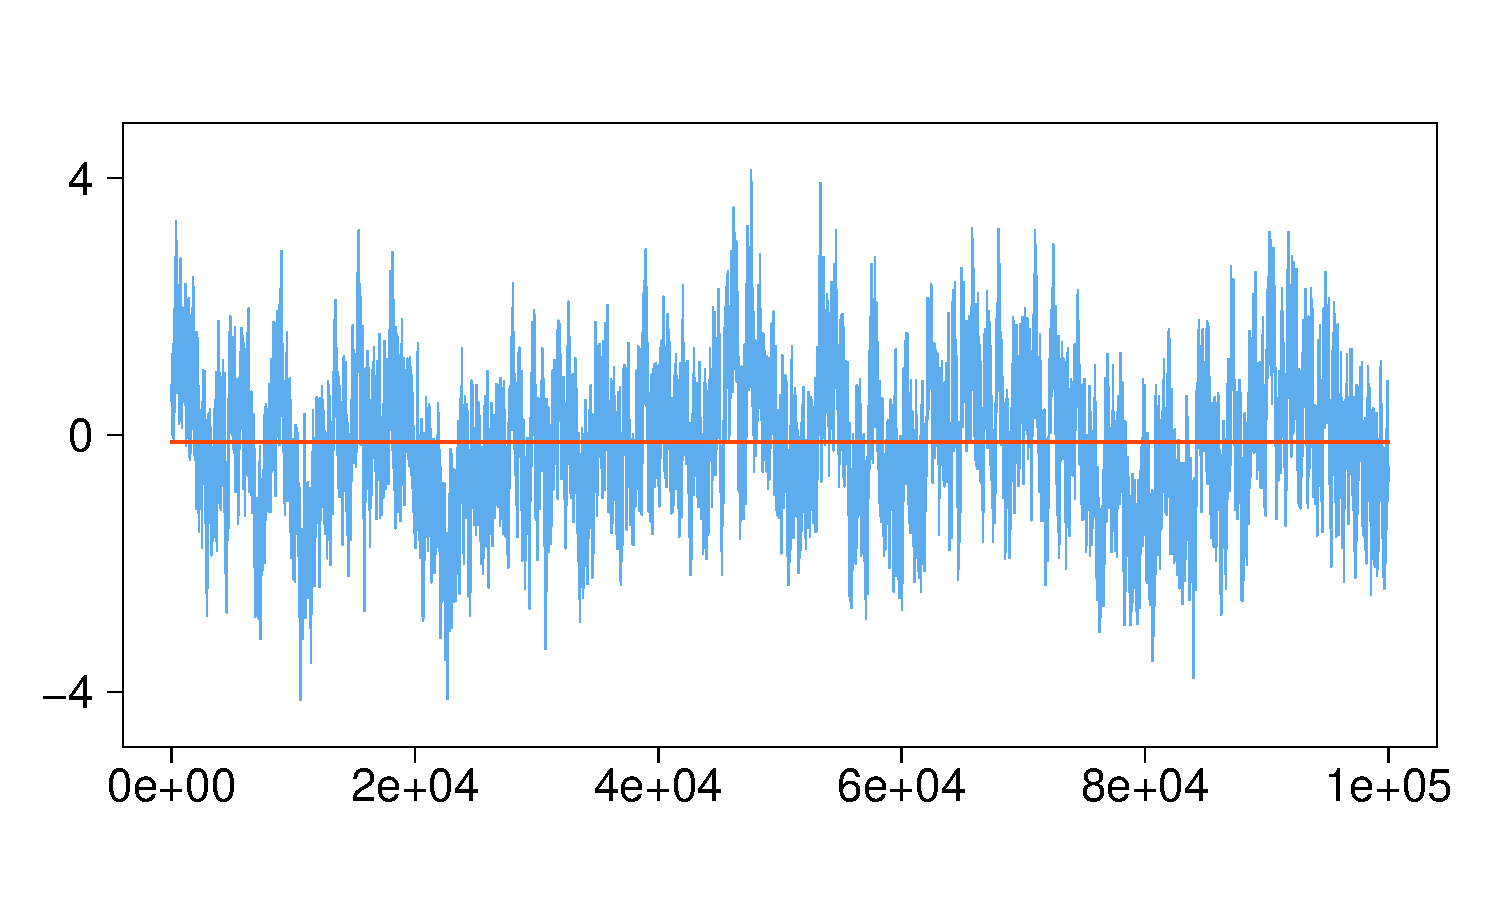
\includegraphics[width=2.8in]{tdist_mala_traceplot.pdf}
	} 
	\subfloat[SMMALA traceplot]{
		\label{fig:t:d}
		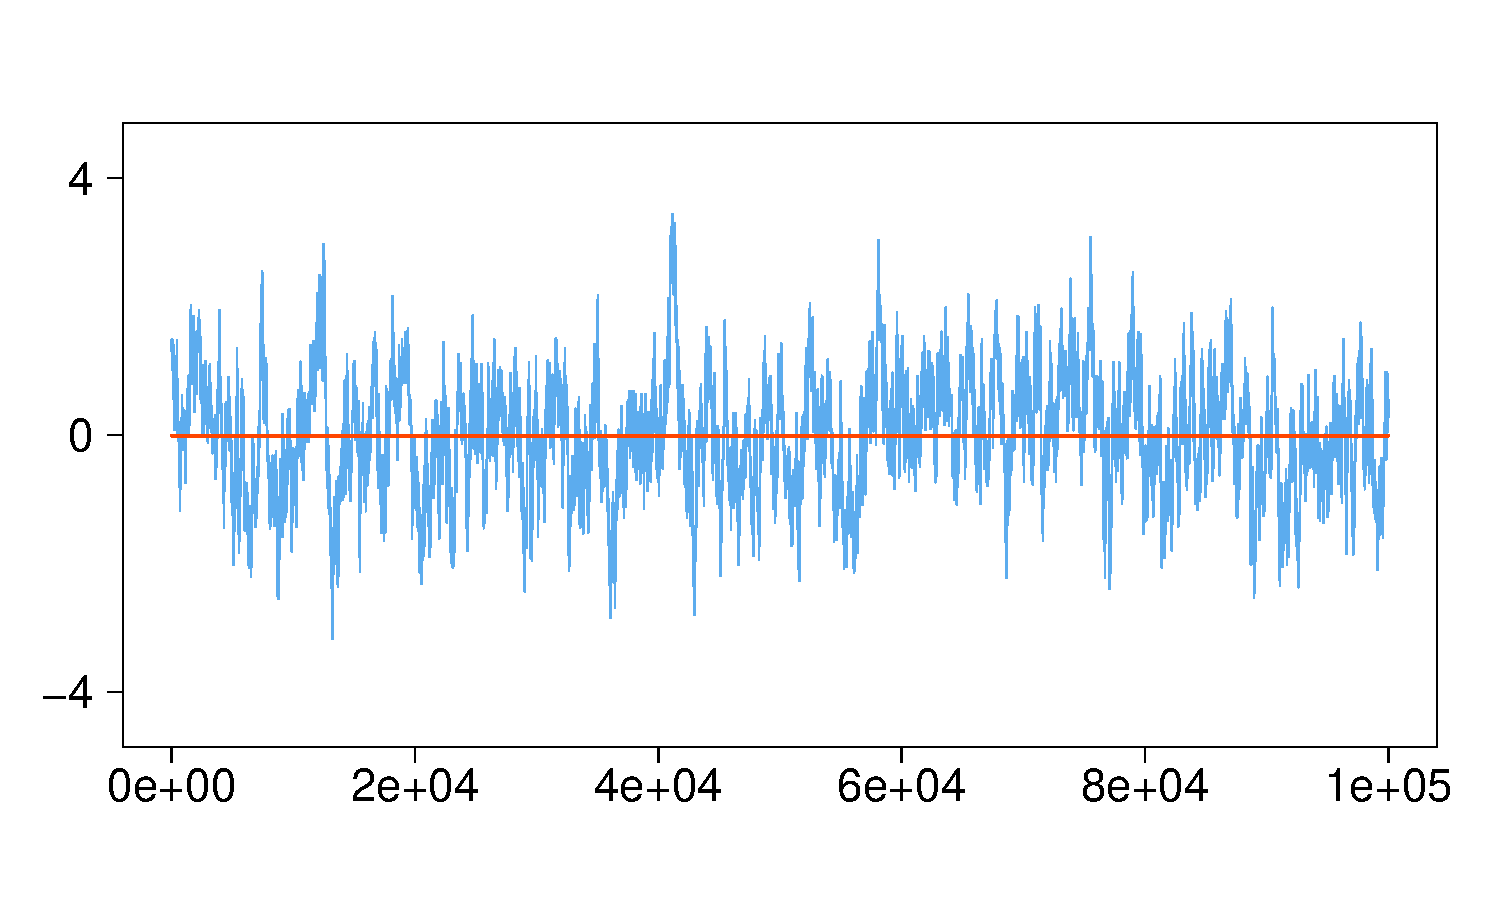
\includegraphics[width=2.8in]{tdist_smmala_traceplot.pdf}
	} \\
	\subfloat[AMSMMALA traceplot]{
		\label{fig:t:e}		
		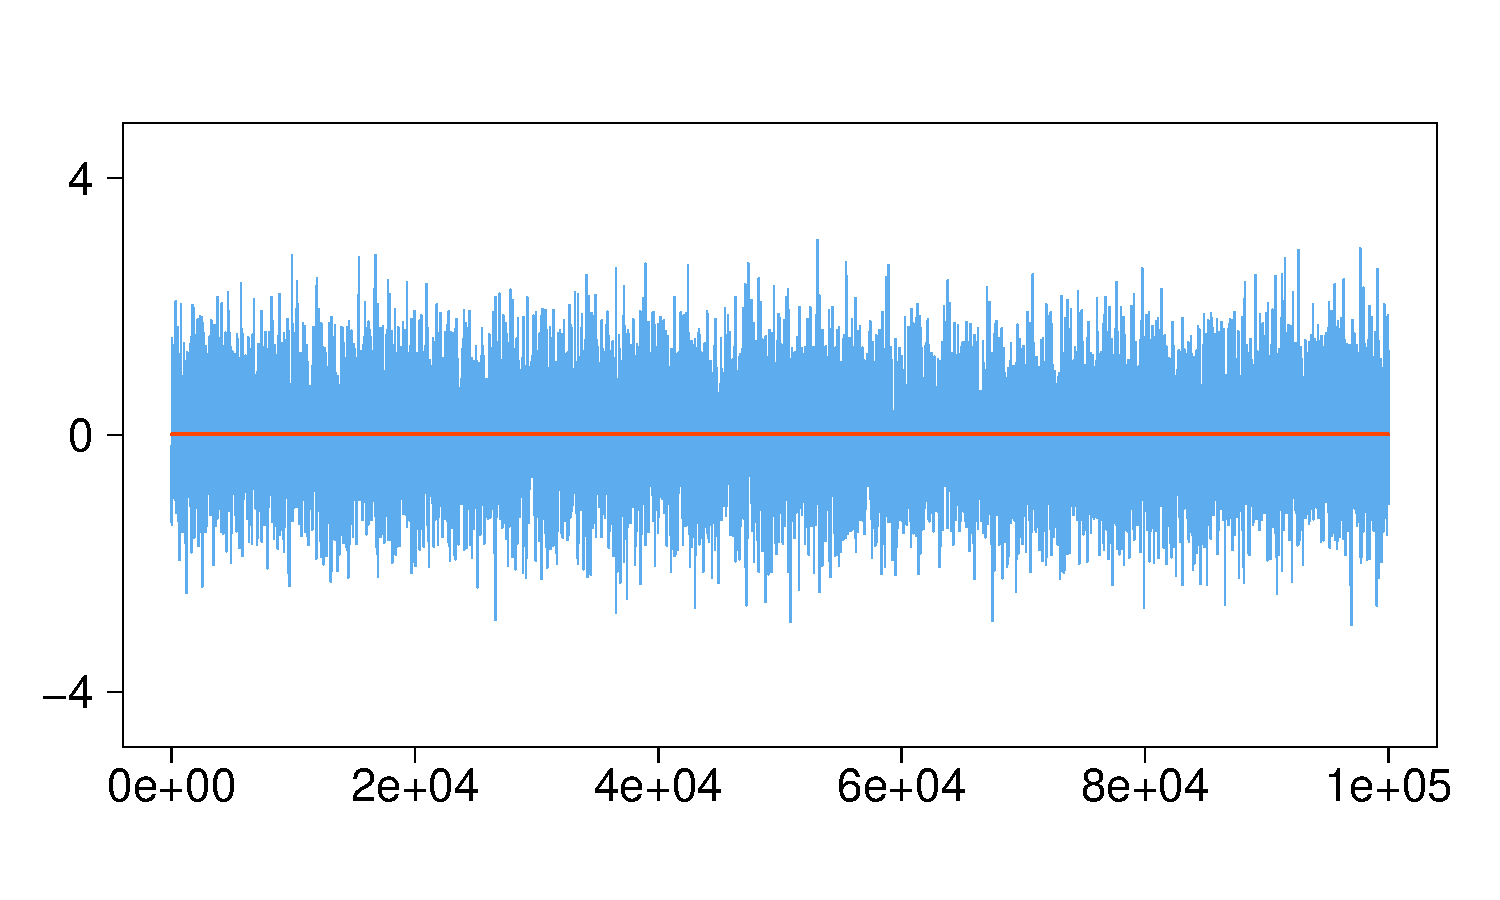
\includegraphics[width=2.8in]{tdist_amsmmala_traceplot.pdf}
	}
	\subfloat[ALSMMALA traceplot]{
		\label{fig:t:f}
		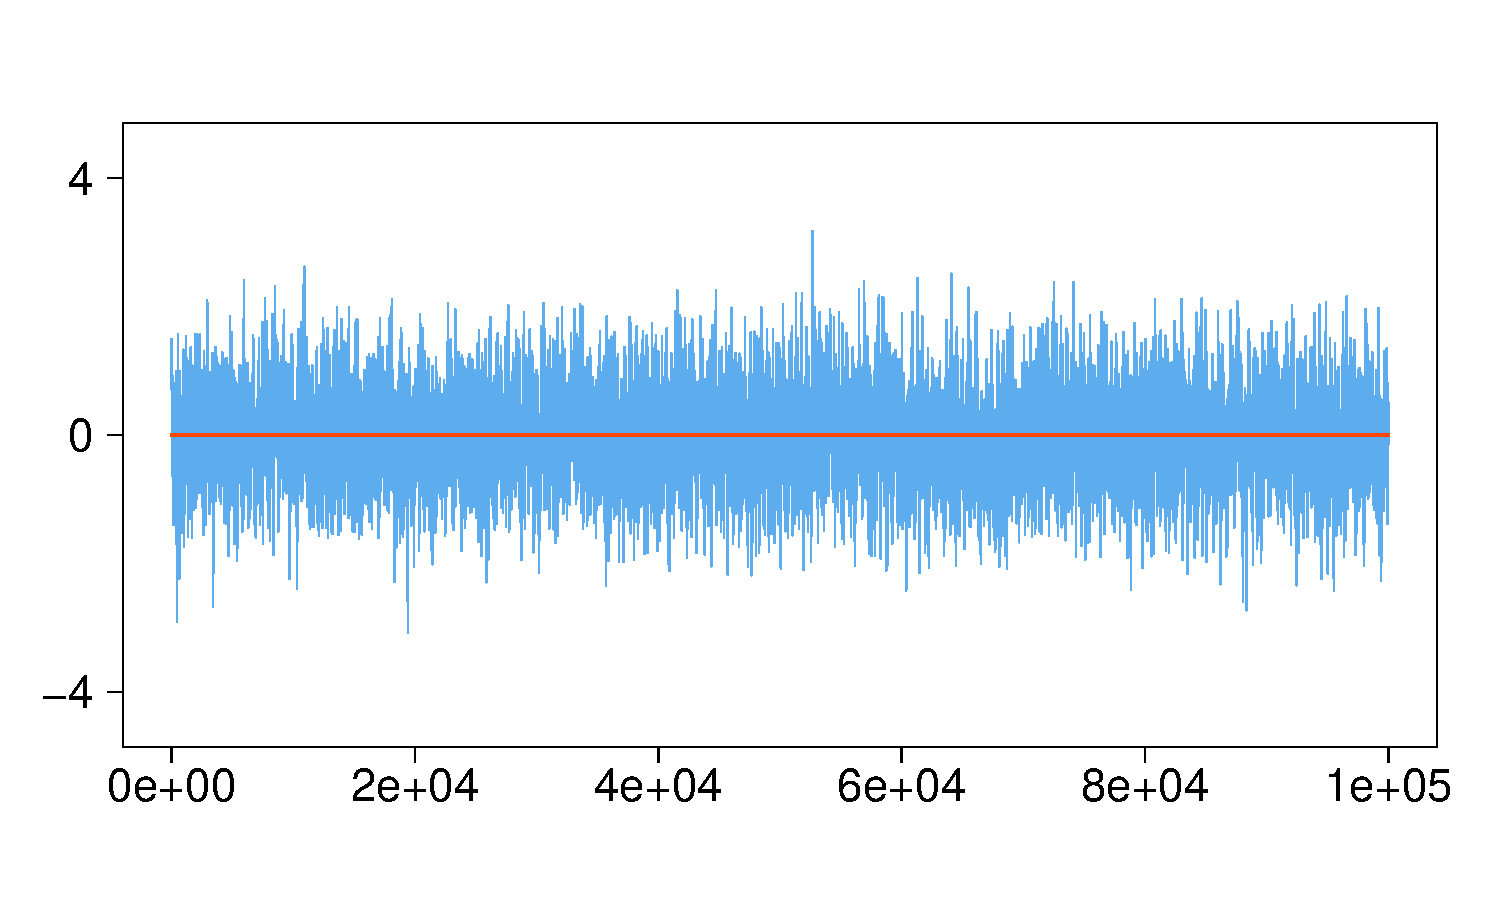
\includegraphics[width=2.8in]{tdist_alsmmala_traceplot.pdf}
	} \\
	\caption{Plots of single chains corresponding to the seventh dimension of the $20$-dimensional $t$-target
		$t_{30}(\mathbf{0},\frac{28}{30}\Sigma(0.9))$ simulated from each of MALA, SMMALA, AMSMMALA and ALSMMALA samplers. (a) 
		Overlaid running means, (b) overlaid linear autocorrelations for the four chains, (c)-(f) individual traceplots per 
		chain (the red horizontal line represent the Monte Carlo mean).}
	\label{fig:t}
\end{figure}

\newpage
\section{Discussion}

MCMC methods have proven critical to the adoption of Bayesian parameter estimation in many scientific and engineering 
disciplines. In the era of big data, researchers are eager to perform inference on models of increasing realism, often 
requiring many model parameters or computationally demanding models. Despite increasing computational resources, there will 
always be a tension between model complexity and computational resources. For many realistic problems, traditional MCMC 
methods can struggle, even in moderately-high dimensional parameter spaces, due to target densities with complex shapes.  
Manifold MCMC algorithms hold considerable promise for improving the efficiency of posterior sampling for such problems.  
However, existing manifold MCMC algorithms can rapidly become prohibitively expensive with increasing dimensionality for 
problems with costly model evaluations of order $\mathcal{O}(f^3(n_{\theta}))$ and $\mathcal{O}(f^2(n_{\theta}))$ for 
MMALA and SMMALA. Therefore, developing geometric MCMC algorithms that are efficient for such problems has the potential to 
enable more realistic models, so as improve the accuracy and robustness of scientific research across multiple disciplines. 

This paper initiates a conceptually straightforward, yet potentially powerful, approach to the problem of making manifold 
MCMC algorithms more accessible with increasing number of parameters. The main idea is to combine proposal mechanisms to 
find a balance between computational complexity and sampling efficacy. TALSMMALA and AMSMMALA have been empirically 
validated on standard statistical models. Even for these computationally trivial examples, the ALSMMALA and AMSMMALA 
algorithms demonstrate considerable promise in terms of performance relative to previous algorithms. The increased effective 
sample size per model evaluation could have an even bigger impact for more complex models which entail more model parameters 
and more expensive model evaluations.  

For example, MCMC methods are essential for the accurate characterization of the masses and orbits of extrasolar planets 
(\cite{for__qua}). For many datasets, a well-chosen random walk Metropolis-Hastings MCMC sampler can be effective 
\cite{for__im}. However, designing an efficient sampler requires considerable human effort for each system. Recently, 
ensemble samplers, such as the differential evolution MCMC (DE-MC) introduced by \cite{bra__ama} and 
adapted by \cite{nel_for_pay__run} and the affine-invariant sampler \cite{hou_goo_hog__ana, mac_hog_lan__emc}, have become 
go-to algorithms for interpreting exoplanet observations, thanks to their balance of computational efficiency and the 
minimal level human effort needed. When analyzing a planetary system containing one star and $n_{\mathrm{pl}}$ planets, 
specifying the model requires at least $n_{\theta} \ge 5\times n_{\mathrm{pl}}-1$ or
$n_{\theta} \ge 7\times n_{\mathrm{pl}}-1$ model parameters depending on whether the orbital planes are assumed to be 
coplanar or potentially inclined, plus additional model parameters for modelling the observing process. Each full model 
evaluation consists of integrating a set of $6\times n_{\mathrm{pl}}$ first-order ordinary differential equations. For some 
planetary systems, the mutual gravitational interactions can be ignored, so using a simpler approximate model can
dramatically reduce the computational cost. However, many of the most scientifically interesting planetary systems and data 
sets require using the full and more expensive model, including Doppler observations of near-resonant planetary systems and 
transit timing measurements for near-resonant or tightly packed systems.

Even if the DE-MC algorithm is parallelized over a cluster of CPUs or a GPU, computing usable posterior samples for such 
systems typically requires weeks of computation
(\cite{doy_car_fab__kep, car_ago_cha__kep, oro_wel_car__kep, nel_for_wri__the, nel_rob_pay__ane, jon_row_lis__the,
jon_for_row__sec, mil_fab_mig__are}.  
Despite these heroic efforts and scientific successes, the resulting effective sample size is often smaller than one would 
like. Further, dozens of scientifically interesting data sets remain unanalyzed (\cite{hol_maz_nac__tra}), largely due to 
the computational cost. For example, the Kepler-57 planetary system has a complex posterior shape (\cite{jon_for_row__sec}) 
that is not well suited to the above ensemble samplers.

Algorithms that exploit geometric information about the posterior shape are likely to be more efficient in terms of the 
number of model evaluations. manifold MCMC methods could make make it practical to generate posterior samples with increased 
effective sample sizes. Unfortunately, computing partial derivatives for every proposal, as required for MMALA or SMMALA, 
would be extremely expensive. The ALSMMALA and AMSMMALA algorithms have the potential to significantly reduce the number of 
gradient and Hessian evaluations required.  

This paper represents one step in the effort to develop more efficient samplers and suggests several future elaborations.  
Other combinations of geometric proposals, such as manifold Hamiltonian Monte Carlo, with computationally cheaper proposals 
can be examined in search of efficient hybrid samplers. Seeking an adaptive or geometrically informed schedule for switching 
between proposal mechanisms could further improve computational efficiency. Another avenue of research would be to apply the 
samplers of this paper to perform thermodynamic integration upon challenging multi-modal posterior densities.   

% Acknowledgements should go at the end, before appendices and references

\acks{  
This paper is based on work supported by the National Aeronautics and Space Administration (NASA) under grant NNX15AE21G 
issued through the Exoplanet Research Program. E.B.F. acknowledges the support of the Eberly College of Science, Center for 
Astrostatistics, Institute for CyberScience and Center for Exoplanets and Habitable Worlds of Pennsylvania State 
University, USA. The Center for Exoplanets and Habitable Worlds is supported by the Pennsylvania State University, the 
Eberly College of Science, and the Pennsylvania Space Grant Consortium. The results reported herein benefited from 
collaborations and/or information exchange within the Nexus for Exoplanet System Science (NExSS) research coordination 
network sponsored by the Science Mission Directorate (SMD) of NASA.
}

% Manual newpage inserted to improve layout of sample file - not
% needed in general before appendices/bibliography.

\newpage

\vskip 0.2in
\bibliography{papamarkou2016}

\end{document}
